% Options for packages loaded elsewhere
\PassOptionsToPackage{unicode}{hyperref}
\PassOptionsToPackage{hyphens}{url}
%
\documentclass[
  11pt,
]{article}
\usepackage{amsmath,amssymb}
\usepackage{setspace}
\usepackage{iftex}
\ifPDFTeX
  \usepackage[T1]{fontenc}
  \usepackage[utf8]{inputenc}
  \usepackage{textcomp} % provide euro and other symbols
\else % if luatex or xetex
  \usepackage{unicode-math} % this also loads fontspec
  \defaultfontfeatures{Scale=MatchLowercase}
  \defaultfontfeatures[\rmfamily]{Ligatures=TeX,Scale=1}
\fi
\usepackage{lmodern}
\ifPDFTeX\else
  % xetex/luatex font selection
\fi
% Use upquote if available, for straight quotes in verbatim environments
\IfFileExists{upquote.sty}{\usepackage{upquote}}{}
\IfFileExists{microtype.sty}{% use microtype if available
  \usepackage[]{microtype}
  \UseMicrotypeSet[protrusion]{basicmath} % disable protrusion for tt fonts
}{}
\makeatletter
\@ifundefined{KOMAClassName}{% if non-KOMA class
  \IfFileExists{parskip.sty}{%
    \usepackage{parskip}
  }{% else
    \setlength{\parindent}{0pt}
    \setlength{\parskip}{6pt plus 2pt minus 1pt}}
}{% if KOMA class
  \KOMAoptions{parskip=half}}
\makeatother
\usepackage{xcolor}
\usepackage[margin=1in]{geometry}
\usepackage{color}
\usepackage{fancyvrb}
\newcommand{\VerbBar}{|}
\newcommand{\VERB}{\Verb[commandchars=\\\{\}]}
\DefineVerbatimEnvironment{Highlighting}{Verbatim}{commandchars=\\\{\}}
% Add ',fontsize=\small' for more characters per line
\usepackage{framed}
\definecolor{shadecolor}{RGB}{248,248,248}
\newenvironment{Shaded}{\begin{snugshade}}{\end{snugshade}}
\newcommand{\AlertTok}[1]{\textcolor[rgb]{0.94,0.16,0.16}{#1}}
\newcommand{\AnnotationTok}[1]{\textcolor[rgb]{0.56,0.35,0.01}{\textbf{\textit{#1}}}}
\newcommand{\AttributeTok}[1]{\textcolor[rgb]{0.13,0.29,0.53}{#1}}
\newcommand{\BaseNTok}[1]{\textcolor[rgb]{0.00,0.00,0.81}{#1}}
\newcommand{\BuiltInTok}[1]{#1}
\newcommand{\CharTok}[1]{\textcolor[rgb]{0.31,0.60,0.02}{#1}}
\newcommand{\CommentTok}[1]{\textcolor[rgb]{0.56,0.35,0.01}{\textit{#1}}}
\newcommand{\CommentVarTok}[1]{\textcolor[rgb]{0.56,0.35,0.01}{\textbf{\textit{#1}}}}
\newcommand{\ConstantTok}[1]{\textcolor[rgb]{0.56,0.35,0.01}{#1}}
\newcommand{\ControlFlowTok}[1]{\textcolor[rgb]{0.13,0.29,0.53}{\textbf{#1}}}
\newcommand{\DataTypeTok}[1]{\textcolor[rgb]{0.13,0.29,0.53}{#1}}
\newcommand{\DecValTok}[1]{\textcolor[rgb]{0.00,0.00,0.81}{#1}}
\newcommand{\DocumentationTok}[1]{\textcolor[rgb]{0.56,0.35,0.01}{\textbf{\textit{#1}}}}
\newcommand{\ErrorTok}[1]{\textcolor[rgb]{0.64,0.00,0.00}{\textbf{#1}}}
\newcommand{\ExtensionTok}[1]{#1}
\newcommand{\FloatTok}[1]{\textcolor[rgb]{0.00,0.00,0.81}{#1}}
\newcommand{\FunctionTok}[1]{\textcolor[rgb]{0.13,0.29,0.53}{\textbf{#1}}}
\newcommand{\ImportTok}[1]{#1}
\newcommand{\InformationTok}[1]{\textcolor[rgb]{0.56,0.35,0.01}{\textbf{\textit{#1}}}}
\newcommand{\KeywordTok}[1]{\textcolor[rgb]{0.13,0.29,0.53}{\textbf{#1}}}
\newcommand{\NormalTok}[1]{#1}
\newcommand{\OperatorTok}[1]{\textcolor[rgb]{0.81,0.36,0.00}{\textbf{#1}}}
\newcommand{\OtherTok}[1]{\textcolor[rgb]{0.56,0.35,0.01}{#1}}
\newcommand{\PreprocessorTok}[1]{\textcolor[rgb]{0.56,0.35,0.01}{\textit{#1}}}
\newcommand{\RegionMarkerTok}[1]{#1}
\newcommand{\SpecialCharTok}[1]{\textcolor[rgb]{0.81,0.36,0.00}{\textbf{#1}}}
\newcommand{\SpecialStringTok}[1]{\textcolor[rgb]{0.31,0.60,0.02}{#1}}
\newcommand{\StringTok}[1]{\textcolor[rgb]{0.31,0.60,0.02}{#1}}
\newcommand{\VariableTok}[1]{\textcolor[rgb]{0.00,0.00,0.00}{#1}}
\newcommand{\VerbatimStringTok}[1]{\textcolor[rgb]{0.31,0.60,0.02}{#1}}
\newcommand{\WarningTok}[1]{\textcolor[rgb]{0.56,0.35,0.01}{\textbf{\textit{#1}}}}
\usepackage{graphicx}
\makeatletter
\def\maxwidth{\ifdim\Gin@nat@width>\linewidth\linewidth\else\Gin@nat@width\fi}
\def\maxheight{\ifdim\Gin@nat@height>\textheight\textheight\else\Gin@nat@height\fi}
\makeatother
% Scale images if necessary, so that they will not overflow the page
% margins by default, and it is still possible to overwrite the defaults
% using explicit options in \includegraphics[width, height, ...]{}
\setkeys{Gin}{width=\maxwidth,height=\maxheight,keepaspectratio}
% Set default figure placement to htbp
\makeatletter
\def\fps@figure{htbp}
\makeatother
\setlength{\emergencystretch}{3em} % prevent overfull lines
\providecommand{\tightlist}{%
  \setlength{\itemsep}{0pt}\setlength{\parskip}{0pt}}
\setcounter{secnumdepth}{5}
\ifLuaTeX
  \usepackage{selnolig}  % disable illegal ligatures
\fi
\usepackage{bookmark}
\IfFileExists{xurl.sty}{\usepackage{xurl}}{} % add URL line breaks if available
\urlstyle{same}
\hypersetup{
  pdftitle={Masters Thesis' Code},
  pdfauthor={Mecki Hamed},
  hidelinks,
  pdfcreator={LaTeX via pandoc}}

\title{Masters Thesis' Code}
\author{Mecki Hamed}
\date{2024-07-25}

\begin{document}
\maketitle

{
\setcounter{tocdepth}{2}
\tableofcontents
}
\setstretch{1.25}
\subsection{1. Limpieza de Datos}\label{limpieza-de-datos}

\subsubsection{1.1 Variables Dependientes}\label{variables-dependientes}

\paragraph{1.1.1 Major Arms - SIPRI}\label{major-arms---sipri}

\begin{Shaded}
\begin{Highlighting}[]
\NormalTok{Volume\_of\_imports\_of\_major\_arms }\OtherTok{\textless{}{-}} \FunctionTok{read\_excel}\NormalTok{(}\StringTok{"import{-}export{-}values\_1990{-}2020.xlsx"}
\NormalTok{)}
\end{Highlighting}
\end{Shaded}

\begin{verbatim}
## New names:
## * `` -> `...2`
## * `` -> `...3`
## * `` -> `...4`
## * `` -> `...5`
## * `` -> `...6`
## * `` -> `...7`
## * `` -> `...8`
## * `` -> `...9`
## * `` -> `...10`
## * `` -> `...11`
## * `` -> `...12`
## * `` -> `...13`
## * `` -> `...14`
## * `` -> `...15`
## * `` -> `...16`
## * `` -> `...17`
## * `` -> `...18`
## * `` -> `...19`
## * `` -> `...20`
## * `` -> `...21`
## * `` -> `...22`
## * `` -> `...23`
## * `` -> `...24`
## * `` -> `...25`
## * `` -> `...26`
## * `` -> `...27`
## * `` -> `...28`
## * `` -> `...29`
## * `` -> `...30`
## * `` -> `...31`
## * `` -> `...32`
## * `` -> `...33`
## * `` -> `...34`
## * `` -> `...35`
## * `` -> `...36`
\end{verbatim}

\begin{Shaded}
\begin{Highlighting}[]
\NormalTok{Volume\_of\_imports\_of\_major\_arms }\OtherTok{\textless{}{-}}\NormalTok{ Volume\_of\_imports\_of\_major\_arms[}\SpecialCharTok{{-}}\FunctionTok{c}\NormalTok{(}\DecValTok{1}\SpecialCharTok{:}\DecValTok{9}\NormalTok{), ]}

\FunctionTok{colnames}\NormalTok{(Volume\_of\_imports\_of\_major\_arms) }\OtherTok{\textless{}{-}} \FunctionTok{c}\NormalTok{(}\StringTok{"Country"}\NormalTok{, }\StringTok{"1990"}\NormalTok{, }\StringTok{"1991"}\NormalTok{, }\StringTok{"1992"}\NormalTok{,}
\StringTok{"1993"}\NormalTok{, }\StringTok{"1994"}\NormalTok{, }\StringTok{"1995"}\NormalTok{, }\StringTok{"1996"}\NormalTok{, }\StringTok{"1997"}\NormalTok{, }\StringTok{"1998"}\NormalTok{, }\StringTok{"1999"}\NormalTok{, }\StringTok{"2000"}\NormalTok{, }\StringTok{"2001"}\NormalTok{, }\StringTok{"2002"}\NormalTok{,}
\StringTok{"2003"}\NormalTok{, }\StringTok{"2004"}\NormalTok{, }\StringTok{"2005"}\NormalTok{, }\StringTok{"2006"}\NormalTok{, }\StringTok{"2007"}\NormalTok{, }\StringTok{"2008"}\NormalTok{, }\StringTok{"2009"}\NormalTok{, }\StringTok{"2010"}\NormalTok{, }\StringTok{"2011"}\NormalTok{, }\StringTok{"2012"}\NormalTok{,}
\StringTok{"2013"}\NormalTok{, }\StringTok{"2014"}\NormalTok{, }\StringTok{"2015"}\NormalTok{, }\StringTok{"2016"}\NormalTok{, }\StringTok{"2017"}\NormalTok{, }\StringTok{"2018"}\NormalTok{, }\StringTok{"2019"}\NormalTok{, }\StringTok{"2020"}\NormalTok{, }\StringTok{"1990{-}2020"}\NormalTok{,}
\StringTok{"Percentage"}\NormalTok{, }\StringTok{"Sum total years"}\NormalTok{, }\StringTok{"Percentage of total"}\NormalTok{)}

\CommentTok{\# Guyana, Costa Rica, Belize, y Honduras tienen muchos NAs, las elimino}

\NormalTok{Volume\_of\_imports\_of\_major\_arms }\OtherTok{\textless{}{-}}\NormalTok{ Volume\_of\_imports\_of\_major\_arms }\SpecialCharTok{|\textgreater{}}
\FunctionTok{filter}\NormalTok{(Country }\SpecialCharTok{\%in\%} \FunctionTok{c}\NormalTok{(}\StringTok{"Argentina"}\NormalTok{, }\StringTok{"Bolivia"}\NormalTok{, }\StringTok{"Brazil"}\NormalTok{, }\StringTok{"Chile"}\NormalTok{, }\StringTok{"Colombia"}\NormalTok{,}
\StringTok{"Ecuador"}\NormalTok{, }\StringTok{"El Salvador"}\NormalTok{, }\StringTok{"Guatemala"}\NormalTok{, }\StringTok{"French Guyana"}\NormalTok{, }\StringTok{"Mexico"}\NormalTok{, }\StringTok{"Nicaragua"}\NormalTok{,}
\StringTok{"Panama"}\NormalTok{, }\StringTok{"Paraguay"}\NormalTok{, }\StringTok{"Peru"}\NormalTok{, }\StringTok{"Uruguay"}\NormalTok{, }\StringTok{"Venezuela"}\NormalTok{)) }\SpecialCharTok{|\textgreater{}}
  \FunctionTok{arrange}\NormalTok{((Country))}

\NormalTok{Volume\_of\_imports\_of\_major\_arms }\OtherTok{\textless{}{-}}\NormalTok{ Volume\_of\_imports\_of\_major\_arms[, }\SpecialCharTok{{-}}\NormalTok{((}\FunctionTok{ncol}\NormalTok{(Volume\_of\_imports\_of\_major\_arms)}\SpecialCharTok{{-}}\DecValTok{3}\NormalTok{)}\SpecialCharTok{:}\FunctionTok{ncol}\NormalTok{(Volume\_of\_imports\_of\_major\_arms))]}

\NormalTok{Volume\_of\_imports\_of\_major\_arms}
\end{Highlighting}
\end{Shaded}

\begin{verbatim}
## # A tibble: 14 x 32
##    Country `1990` `1991` `1992` `1993` `1994` `1995` `1996` `1997` `1998` `1999`
##    <chr>    <dbl>  <dbl>  <dbl>  <dbl>  <dbl>  <dbl>  <dbl>  <dbl>  <dbl>  <dbl>
##  1 Argent~    159     NA     27     NA    209     43     21    105    171    276
##  2 Bolivia     NA     11     25     16      9      2     NA     NA     NA      9
##  3 Brazil     136    160     91     57    306    241    536    465    232    376
##  4 Chile      135    104    170     85     82    331    164    284     88    206
##  5 Colomb~     13     72     36     68     42     35     49    193    160     44
##  6 Ecuador      3    136      4     18     17     45     29    103     31     16
##  7 El Sal~     NA     21      4      2     NA      4      4     NA      2     NA
##  8 Guatem~      0      0     NA     13      4      4      2     NA      1     NA
##  9 Mexico      34     40     19    160    136     55     92    495     19    136
## 10 Nicara~    107      1     NA     NA     NA     NA     NA     NA     NA     NA
## 11 Paragu~      6      3      1     NA     NA     NA      2     NA     NA     NA
## 12 Peru       104    108    130     43    175     47    121    373     51     94
## 13 Uruguay     41     63     25     18     11     12      4     19     27      9
## 14 Venezu~    189    318     72     37      1      5     37     39      8     85
## # i 21 more variables: `2000` <dbl>, `2001` <dbl>, `2002` <dbl>, `2003` <dbl>,
## #   `2004` <dbl>, `2005` <dbl>, `2006` <dbl>, `2007` <dbl>, `2008` <dbl>,
## #   `2009` <dbl>, `2010` <dbl>, `2011` <dbl>, `2012` <dbl>, `2013` <dbl>,
## #   `2014` <dbl>, `2015` <dbl>, `2016` <dbl>, `2017` <dbl>, `2018` <dbl>,
## #   `2019` <dbl>, `2020` <dbl>
\end{verbatim}

\paragraph{1.1.2 Small Arms - UNROCA}\label{small-arms---unroca}

\begin{Shaded}
\begin{Highlighting}[]
\NormalTok{small\_arms\_unroca }\OtherTok{\textless{}{-}} \FunctionTok{read\_excel}\NormalTok{(}\StringTok{"small\_arms\_unroca.xlsx"}\NormalTok{)}

\NormalTok{small\_arms\_unroca }\OtherTok{\textless{}{-}}\NormalTok{ small\_arms\_unroca[, }\SpecialCharTok{{-}}\FunctionTok{c}\NormalTok{(}\DecValTok{2}\SpecialCharTok{:}\DecValTok{17}\NormalTok{)]}

\NormalTok{small\_arms\_unroca }\OtherTok{\textless{}{-}}\NormalTok{ small\_arms\_unroca }\SpecialCharTok{|\textgreater{}}
\FunctionTok{filter}\NormalTok{(Country }\SpecialCharTok{\%in\%} \FunctionTok{c}\NormalTok{(}\StringTok{"Argentina"}\NormalTok{, }\StringTok{"Bolivia"}\NormalTok{, }\StringTok{"Brazil"}\NormalTok{, }\StringTok{"Chile"}\NormalTok{, }\StringTok{"Colombia"}\NormalTok{,}
\StringTok{"Ecuador"}\NormalTok{, }\StringTok{"El Salvador"}\NormalTok{, }\StringTok{"Guatemala"}\NormalTok{, }\StringTok{"French Guyana"}\NormalTok{, }\StringTok{"Mexico"}\NormalTok{, }\StringTok{"Nicaragua"}\NormalTok{,}
\StringTok{"Panama"}\NormalTok{, }\StringTok{"Paraguay"}\NormalTok{, }\StringTok{"Peru"}\NormalTok{, }\StringTok{"Uruguay"}\NormalTok{, }\StringTok{"Venezuela"}\NormalTok{)) }\SpecialCharTok{|\textgreater{}}
  \FunctionTok{arrange}\NormalTok{((Country))}

\NormalTok{small\_arms\_unroca }\OtherTok{\textless{}{-}}\NormalTok{ small\_arms\_unroca[, }\SpecialCharTok{{-}}\NormalTok{((}\FunctionTok{ncol}\NormalTok{(small\_arms\_unroca)}\SpecialCharTok{{-}}\DecValTok{3}\NormalTok{)}\SpecialCharTok{:}\FunctionTok{ncol}\NormalTok{(small\_arms\_unroca))]}

\NormalTok{small\_arms\_unroca}
\end{Highlighting}
\end{Shaded}

\begin{verbatim}
## # A tibble: 14 x 16
##    Country `2006` `2007` `2008` `2009` `2010` `2011` `2012` `2013` `2014` `2015`
##    <chr>    <dbl>  <dbl>  <dbl>  <dbl>  <dbl>  <dbl>  <dbl>  <dbl>  <dbl>  <dbl>
##  1 Argent~    130   6114   9350   3975   4275    228    245   2597   5472  12729
##  2 Bolivia     NA     18   1078     NA     NA     NA     NA    461    100    552
##  3 Brazil     725    144    159    140  48077    540    879    514   3923   2386
##  4 Chile       26   2947    106    493   1156     68    327   1482   6411   2325
##  5 Colomb~    750   1766   2757   2150    949      1    167   3108   2554     40
##  6 Ecuador     51    193     55   3890     NA     NA     NA     NA  15009    377
##  7 El Sal~    340     59     NA     13    325     55     40    242    174     40
##  8 Guatem~    500   2718   7976    310    640    225   1360  18548   1842    725
##  9 Mexico     673  55859  49143  56936  39973  30173  38321  80872  49003  42601
## 10 Nicara~     NA     50    840     NA    504    150    495     50     NA    215
## 11 Paragu~     NA     NA     30     40   1307    103    645   2637    135   2002
## 12 Peru        30    541   1244    506   6860      8   6863   2011   1336  20211
## 13 Uruguay     50    249    959    589   1938      7     NA    304   1136  11616
## 14 Venezu~     30   7678   8390  17026     16     NA     80   7980     26     NA
## # i 5 more variables: `2016` <dbl>, `2017` <dbl>, `2018` <dbl>, `2019` <dbl>,
## #   `2020` <dbl>
\end{verbatim}

\subsubsection{1.2 Variables
Independientes}\label{variables-independientes}

\paragraph{1.2.1 Political Events -
ACLED}\label{political-events---acled}

\begin{Shaded}
\begin{Highlighting}[]
\NormalTok{ACLED\_events }\OtherTok{\textless{}{-}} \FunctionTok{read\_excel}\NormalTok{(}\StringTok{"ACLED\_central\_and\_south\_america\_events.xlsx"}\NormalTok{)}
\end{Highlighting}
\end{Shaded}

\begin{verbatim}
## Warning: Expecting numeric in X37572 / R37572C24: got '-1.094.262'
\end{verbatim}

\begin{verbatim}
## Warning: Expecting numeric in X39359 / R39359C24: got '-1.094.262'
\end{verbatim}

\begin{verbatim}
## Warning: Expecting numeric in X53448 / R53448C24: got '-1.094.262'
\end{verbatim}

\begin{Shaded}
\begin{Highlighting}[]
\NormalTok{paises\_de\_estudio }\OtherTok{\textless{}{-}} \FunctionTok{c}\NormalTok{(}\StringTok{"Argentina"}\NormalTok{, }\StringTok{"Bolivia"}\NormalTok{, }\StringTok{"Brazil"}\NormalTok{, }\StringTok{"Chile"}\NormalTok{, }\StringTok{"Colombia"}\NormalTok{,}
\StringTok{"Ecuador"}\NormalTok{, }\StringTok{"El Salvador"}\NormalTok{, }\StringTok{"Guatemala"}\NormalTok{, }\StringTok{"French Guyana"}\NormalTok{, }\StringTok{"Mexico"}\NormalTok{, }\StringTok{"Nicaragua"}\NormalTok{,}
\StringTok{"Panama"}\NormalTok{, }\StringTok{"Paraguay"}\NormalTok{, }\StringTok{"Peru"}\NormalTok{, }\StringTok{"Uruguay"}\NormalTok{, }\StringTok{"Venezuela"}\NormalTok{)}

\NormalTok{ACLED\_events }\OtherTok{\textless{}{-}}\NormalTok{ ACLED\_events[ACLED\_events}\SpecialCharTok{$}\NormalTok{country }\SpecialCharTok{\%in\%}\NormalTok{ paises\_de\_estudio, ]}

\CommentTok{\#eliminar peaceful protest}

\NormalTok{ACLED\_events }\OtherTok{\textless{}{-}}\NormalTok{ ACLED\_events }\SpecialCharTok{|\textgreater{}}
  \FunctionTok{filter}\NormalTok{(sub\_event\_type }\SpecialCharTok{!=} \StringTok{"Peaceful protest"}\NormalTok{)}

\NormalTok{ACLED\_events }\OtherTok{\textless{}{-}}\NormalTok{ ACLED\_events }\SpecialCharTok{\%\textgreater{}\%}
  \FunctionTok{group\_by}\NormalTok{(country, year) }\SpecialCharTok{\%\textgreater{}\%}
  \FunctionTok{summarise}\NormalTok{(}\AttributeTok{conflict\_count =} \FunctionTok{n}\NormalTok{()) }\SpecialCharTok{\%\textgreater{}\%}
  \FunctionTok{ungroup}\NormalTok{() }\SpecialCharTok{\%\textgreater{}\%}
  \FunctionTok{pivot\_wider}\NormalTok{(}\AttributeTok{names\_from =}\NormalTok{ year, }\AttributeTok{values\_from =}\NormalTok{ conflict\_count, }\AttributeTok{values\_fill =} \DecValTok{0}\NormalTok{) }\SpecialCharTok{|\textgreater{}}
  \FunctionTok{rename}\NormalTok{(}\AttributeTok{Country =}\NormalTok{ country)}
\end{Highlighting}
\end{Shaded}

\begin{verbatim}
## `summarise()` has grouped output by 'country'. You can override using the
## `.groups` argument.
\end{verbatim}

\begin{Shaded}
\begin{Highlighting}[]
\NormalTok{ACLED\_Political\_events }\OtherTok{\textless{}{-}}\NormalTok{ ACLED\_events}

\NormalTok{ACLED\_Political\_events}
\end{Highlighting}
\end{Shaded}

\begin{verbatim}
## # A tibble: 14 x 4
##    Country     `2018` `2019` `2020`
##    <chr>        <int>  <int>  <int>
##  1 Argentina      189    157    183
##  2 Bolivia         56    154    122
##  3 Brazil       11019   8893   8310
##  4 Chile          476   1309    993
##  5 Colombia      2076   2075   2061
##  6 Ecuador         34     94     54
##  7 El Salvador    797    828    398
##  8 Guatemala      873   1247    738
##  9 Nicaragua      273    106     77
## 10 Panama          52     37     32
## 11 Paraguay        50     81     76
## 12 Peru           115    210    318
## 13 Uruguay         10     17      9
## 14 Venezuela     1317   1972   1698
\end{verbatim}

\paragraph{1.2.2 Armed Conflicts - UCDP /
PRIO}\label{armed-conflicts---ucdp-prio}

\begin{Shaded}
\begin{Highlighting}[]
\NormalTok{UcdpPrioConflict\_v24\_1 }\OtherTok{\textless{}{-}} \FunctionTok{read\_excel}\NormalTok{(}\StringTok{"UcdpPrioConflict\_v24\_1.xlsx"}\NormalTok{)}

\NormalTok{conflict\_filtrados }\OtherTok{\textless{}{-}}\NormalTok{ UcdpPrioConflict\_v24\_1[UcdpPrioConflict\_v24\_1}\SpecialCharTok{$}\NormalTok{location }\SpecialCharTok{\%in\%}\NormalTok{ paises\_de\_estudio, ]}


\NormalTok{conflict\_filtrados }\OtherTok{\textless{}{-}}\NormalTok{ conflict\_filtrados[conflict\_filtrados}\SpecialCharTok{$}\NormalTok{year }\SpecialCharTok{\textgreater{}=} \DecValTok{1990} \SpecialCharTok{\&}\NormalTok{ conflict\_filtrados}\SpecialCharTok{$}\NormalTok{year }\SpecialCharTok{\textless{}=} \DecValTok{2020}\NormalTok{, ]}


\NormalTok{conflict\_filtrados }\OtherTok{\textless{}{-}}\NormalTok{ conflict\_filtrados }\SpecialCharTok{\%\textgreater{}\%}
  \FunctionTok{group\_by}\NormalTok{(location, year) }\SpecialCharTok{\%\textgreater{}\%}
  \FunctionTok{summarise}\NormalTok{(}\AttributeTok{conflict\_count =} \FunctionTok{n}\NormalTok{()) }\SpecialCharTok{\%\textgreater{}\%}
  \FunctionTok{ungroup}\NormalTok{() }\SpecialCharTok{\%\textgreater{}\%}
  \FunctionTok{pivot\_wider}\NormalTok{(}\AttributeTok{names\_from =}\NormalTok{ year, }\AttributeTok{values\_from =}\NormalTok{ conflict\_count, }\AttributeTok{values\_fill =} \DecValTok{0}\NormalTok{) }\SpecialCharTok{|\textgreater{}}
    \FunctionTok{rename}\NormalTok{(}\AttributeTok{Country =}\NormalTok{ location) }\SpecialCharTok{\%\textgreater{}\%}
  \FunctionTok{mutate}\NormalTok{(}\FunctionTok{across}\NormalTok{(}\SpecialCharTok{{-}}\NormalTok{Country, as.double)) }\SpecialCharTok{|\textgreater{}}
  \FunctionTok{arrange}\NormalTok{(Country)}
\end{Highlighting}
\end{Shaded}

\begin{verbatim}
## `summarise()` has grouped output by 'location'. You can override using the
## `.groups` argument.
\end{verbatim}

\begin{Shaded}
\begin{Highlighting}[]
\NormalTok{conflict\_filtrados}\SpecialCharTok{$}\StringTok{\textasciigrave{}}\AttributeTok{2017}\StringTok{\textasciigrave{}} \OtherTok{\textless{}{-}} \DecValTok{0}

\NormalTok{conflict\_filtrados }\OtherTok{\textless{}{-}}\NormalTok{ conflict\_filtrados[, }\FunctionTok{c}\NormalTok{(}\FunctionTok{names}\NormalTok{(conflict\_filtrados)[}\DecValTok{1}\SpecialCharTok{:}\FunctionTok{which}\NormalTok{(}\FunctionTok{names}\NormalTok{(conflict\_filtrados) }\SpecialCharTok{==} \StringTok{"2016"}\NormalTok{)], }\StringTok{"2017"}\NormalTok{, }\FunctionTok{names}\NormalTok{(conflict\_filtrados)[(}\FunctionTok{which}\NormalTok{(}\FunctionTok{names}\NormalTok{(conflict\_filtrados) }\SpecialCharTok{==} \StringTok{"2016"}\NormalTok{) }\SpecialCharTok{+} \DecValTok{1}\NormalTok{)}\SpecialCharTok{:}\FunctionTok{ncol}\NormalTok{(conflict\_filtrados)])]}
\NormalTok{conflict\_filtrados }\OtherTok{\textless{}{-}}\NormalTok{ conflict\_filtrados[, }\SpecialCharTok{{-}}\FunctionTok{ncol}\NormalTok{(conflict\_filtrados)]}

\NormalTok{PRIO\_Armed\_Conflicts }\OtherTok{\textless{}{-}}\NormalTok{ conflict\_filtrados}

\NormalTok{PRIO\_Armed\_Conflicts}
\end{Highlighting}
\end{Shaded}

\begin{verbatim}
## # A tibble: 7 x 32
##   Country  `1990` `1991` `1992` `1993` `1994` `1995` `1996` `1997` `1998` `1999`
##   <chr>     <dbl>  <dbl>  <dbl>  <dbl>  <dbl>  <dbl>  <dbl>  <dbl>  <dbl>  <dbl>
## 1 Colombia      1      1      1      1      1      1      1      1      1      1
## 2 El Salv~      1      1      0      0      0      0      0      0      0      0
## 3 Guatema~      1      1      1      1      1      1      0      0      0      0
## 4 Mexico        0      0      0      0      1      0      1      0      0      0
## 5 Nicarag~      1      0      0      0      0      0      0      0      0      0
## 6 Peru          1      1      1      1      1      1      1      1      1      1
## 7 Venezue~      0      0      1      0      0      0      0      0      0      0
## # i 21 more variables: `2000` <dbl>, `2001` <dbl>, `2002` <dbl>, `2003` <dbl>,
## #   `2004` <dbl>, `2005` <dbl>, `2006` <dbl>, `2007` <dbl>, `2008` <dbl>,
## #   `2009` <dbl>, `2010` <dbl>, `2011` <dbl>, `2012` <dbl>, `2013` <dbl>,
## #   `2014` <dbl>, `2015` <dbl>, `2016` <dbl>, `2017` <dbl>, `2018` <dbl>,
## #   `2019` <dbl>, `2020` <dbl>
\end{verbatim}

\paragraph{1.2.3 Non-State Violence -
UCDP/PRIO}\label{non-state-violence---ucdpprio}

\begin{Shaded}
\begin{Highlighting}[]
\NormalTok{Nonstate\_v24\_1 }\OtherTok{\textless{}{-}} \FunctionTok{read\_excel}\NormalTok{(}\StringTok{"Nonstate\_v24\_1.xlsx"}\NormalTok{)}

\NormalTok{non\_state\_filtrados }\OtherTok{\textless{}{-}}\NormalTok{ Nonstate\_v24\_1[Nonstate\_v24\_1}\SpecialCharTok{$}\NormalTok{location }\SpecialCharTok{\%in\%}\NormalTok{ paises\_de\_estudio, ]}

\NormalTok{non\_state\_filtrados }\OtherTok{\textless{}{-}}\NormalTok{ non\_state\_filtrados[non\_state\_filtrados}\SpecialCharTok{$}\NormalTok{year }\SpecialCharTok{\textgreater{}=} \DecValTok{1990} \SpecialCharTok{\&}\NormalTok{ non\_state\_filtrados}\SpecialCharTok{$}\NormalTok{year }\SpecialCharTok{\textless{}=} \DecValTok{2020}\NormalTok{, ]}

\NormalTok{non\_state\_filtrados }\OtherTok{\textless{}{-}}\NormalTok{ non\_state\_filtrados }\SpecialCharTok{\%\textgreater{}\%}
  \FunctionTok{group\_by}\NormalTok{(location, year) }\SpecialCharTok{\%\textgreater{}\%}
  \FunctionTok{summarise}\NormalTok{(}\AttributeTok{conflict\_count =} \FunctionTok{n}\NormalTok{()) }\SpecialCharTok{\%\textgreater{}\%}
  \FunctionTok{ungroup}\NormalTok{() }\SpecialCharTok{\%\textgreater{}\%}
  \FunctionTok{pivot\_wider}\NormalTok{(}\AttributeTok{names\_from =}\NormalTok{ year, }\AttributeTok{values\_from =}\NormalTok{ conflict\_count, }\AttributeTok{values\_fill =} \DecValTok{0}\NormalTok{) }\SpecialCharTok{|\textgreater{}}
    \FunctionTok{rename}\NormalTok{(}\AttributeTok{Country =}\NormalTok{ location) }\SpecialCharTok{\%\textgreater{}\%}
  \FunctionTok{mutate}\NormalTok{(}\FunctionTok{across}\NormalTok{(}\SpecialCharTok{{-}}\NormalTok{Country, as.double)) }
\end{Highlighting}
\end{Shaded}

\begin{verbatim}
## `summarise()` has grouped output by 'location'. You can override using the
## `.groups` argument.
\end{verbatim}

\begin{Shaded}
\begin{Highlighting}[]
\NormalTok{non\_state\_filtrados\_columnas\_ordenadas }\OtherTok{\textless{}{-}} \FunctionTok{c}\NormalTok{(}\StringTok{"Country"}\NormalTok{, }\FunctionTok{sort}\NormalTok{(}\FunctionTok{as.numeric}\NormalTok{(}\FunctionTok{names}\NormalTok{(non\_state\_filtrados)[}\SpecialCharTok{{-}}\DecValTok{1}\NormalTok{])))}

\NormalTok{non\_state\_filtrados }\OtherTok{\textless{}{-}}\NormalTok{ non\_state\_filtrados[, non\_state\_filtrados\_columnas\_ordenadas]}

\CommentTok{\# Crear las columnas "1992" y "1996" con valores de 0 o NA en funcion de si decimos que no hay registros porque no hay eventos, o si decimos que no hay registros simplemente}

\NormalTok{non\_state\_filtrados}\SpecialCharTok{$}\StringTok{\textasciigrave{}}\AttributeTok{1992}\StringTok{\textasciigrave{}} \OtherTok{\textless{}{-}} \ConstantTok{NA}
\NormalTok{non\_state\_filtrados}\SpecialCharTok{$}\StringTok{\textasciigrave{}}\AttributeTok{1996}\StringTok{\textasciigrave{}} \OtherTok{\textless{}{-}} \ConstantTok{NA}

\NormalTok{non\_state\_filtrados }\OtherTok{\textless{}{-}}\NormalTok{ non\_state\_filtrados[, }\FunctionTok{c}\NormalTok{(}\FunctionTok{names}\NormalTok{(non\_state\_filtrados)[}\DecValTok{1}\SpecialCharTok{:}\FunctionTok{which}\NormalTok{(}\FunctionTok{names}\NormalTok{(non\_state\_filtrados) }\SpecialCharTok{==} \StringTok{"1991"}\NormalTok{)], }
                                               \StringTok{"1992"}\NormalTok{, }
                                               \FunctionTok{names}\NormalTok{(non\_state\_filtrados)[(}\FunctionTok{which}\NormalTok{(}\FunctionTok{names}\NormalTok{(non\_state\_filtrados) }\SpecialCharTok{==} \StringTok{"1991"}\NormalTok{) }\SpecialCharTok{+} \DecValTok{1}\NormalTok{)}\SpecialCharTok{:}\FunctionTok{which}\NormalTok{(}\FunctionTok{names}\NormalTok{(non\_state\_filtrados) }\SpecialCharTok{==} \StringTok{"1995"}\NormalTok{)], }
                                               \StringTok{"1996"}\NormalTok{, }
                                               \FunctionTok{names}\NormalTok{(non\_state\_filtrados)[(}\FunctionTok{which}\NormalTok{(}\FunctionTok{names}\NormalTok{(non\_state\_filtrados) }\SpecialCharTok{==} \StringTok{"1995"}\NormalTok{) }\SpecialCharTok{+} \DecValTok{1}\NormalTok{)}\SpecialCharTok{:}\FunctionTok{ncol}\NormalTok{(non\_state\_filtrados)])]}

\NormalTok{non\_state\_filtrados }\OtherTok{\textless{}{-}}\NormalTok{ non\_state\_filtrados[, }\SpecialCharTok{{-}}\NormalTok{((}\FunctionTok{ncol}\NormalTok{(non\_state\_filtrados)}\SpecialCharTok{{-}}\DecValTok{1}\NormalTok{)}\SpecialCharTok{:}\FunctionTok{ncol}\NormalTok{(non\_state\_filtrados))]}

\NormalTok{PRIO\_Non\_State\_Conflicts }\OtherTok{\textless{}{-}}\NormalTok{ non\_state\_filtrados}

\NormalTok{PRIO\_Non\_State\_Conflicts}
\end{Highlighting}
\end{Shaded}

\begin{verbatim}
## # A tibble: 9 x 32
##   Country  `1990` `1991` `1992` `1993` `1994` `1995` `1996` `1997` `1998` `1999`
##   <chr>     <dbl>  <dbl> <lgl>   <dbl>  <dbl>  <dbl> <lgl>   <dbl>  <dbl>  <dbl>
## 1 Bolivia       0      0 NA          0      0      0 NA          0      0      0
## 2 Brazil        0      0 NA          0      1      1 NA          1      0      1
## 3 Colombia      1      0 NA          1      0      0 NA          1      2      1
## 4 Ecuador       0      0 NA          0      0      0 NA          0      0      0
## 5 El Salv~      0      0 NA          0      0      0 NA          0      0      0
## 6 Guatema~      0      0 NA          0      0      0 NA          0      0      0
## 7 Mexico        0      0 NA          1      0      0 NA          0      0      0
## 8 Peru          0      1 NA          0      0      0 NA          0      0      0
## 9 Venezue~      0      0 NA          0      1      0 NA          1      0      0
## # i 21 more variables: `2000` <dbl>, `2001` <dbl>, `2002` <dbl>, `2003` <dbl>,
## #   `2004` <dbl>, `2005` <dbl>, `2006` <dbl>, `2007` <dbl>, `2008` <dbl>,
## #   `2009` <dbl>, `2010` <dbl>, `2011` <dbl>, `2012` <dbl>, `2013` <dbl>,
## #   `2014` <dbl>, `2015` <dbl>, `2016` <dbl>, `2017` <dbl>, `2018` <dbl>,
## #   `2019` <dbl>, `2020` <dbl>
\end{verbatim}

\paragraph{1.2.4 Deadly Electoral Events - UCDP /
PRIO}\label{deadly-electoral-events---ucdp-prio}

\begin{Shaded}
\begin{Highlighting}[]
\NormalTok{DECO\_v\_1\_0 }\OtherTok{\textless{}{-}} \FunctionTok{read\_excel}\NormalTok{(}\StringTok{"DECO\_v.1.0.xlsx"}\NormalTok{)}
\end{Highlighting}
\end{Shaded}

\begin{verbatim}
## Warning: Expecting logical in AH2344 / R2344C34: got 'Political supporters'
\end{verbatim}

\begin{verbatim}
## Warning: Expecting logical in AH2448 / R2448C34: got 'Security forces'
\end{verbatim}

\begin{Shaded}
\begin{Highlighting}[]
\NormalTok{DECO\_v\_1\_0\_filtrados }\OtherTok{\textless{}{-}}\NormalTok{ DECO\_v\_1\_0[DECO\_v\_1\_0}\SpecialCharTok{$}\NormalTok{country }\SpecialCharTok{\%in\%}\NormalTok{ paises\_de\_estudio, ]}

\NormalTok{DECO\_v\_1\_0\_filtrados }\OtherTok{\textless{}{-}}\NormalTok{ DECO\_v\_1\_0\_filtrados[DECO\_v\_1\_0\_filtrados}\SpecialCharTok{$}\NormalTok{year }\SpecialCharTok{\textgreater{}=} \DecValTok{1990} \SpecialCharTok{\&}\NormalTok{ DECO\_v\_1\_0\_filtrados}\SpecialCharTok{$}\NormalTok{year }\SpecialCharTok{\textless{}=} \DecValTok{2020}\NormalTok{, ]}

\NormalTok{DECO\_v\_1\_0\_filtrados }\OtherTok{\textless{}{-}}\NormalTok{ DECO\_v\_1\_0\_filtrados }\SpecialCharTok{\%\textgreater{}\%}
  \FunctionTok{group\_by}\NormalTok{(country, year) }\SpecialCharTok{\%\textgreater{}\%}
  \FunctionTok{summarise}\NormalTok{(}\AttributeTok{conflict\_count =} \FunctionTok{n}\NormalTok{()) }\SpecialCharTok{\%\textgreater{}\%}
  \FunctionTok{ungroup}\NormalTok{() }\SpecialCharTok{|\textgreater{}}
  \FunctionTok{pivot\_wider}\NormalTok{(}\AttributeTok{names\_from =}\NormalTok{ year, }\AttributeTok{values\_from =}\NormalTok{ conflict\_count, }\AttributeTok{values\_fill =} \DecValTok{0}\NormalTok{) }\SpecialCharTok{|\textgreater{}}
    \FunctionTok{rename}\NormalTok{(}\AttributeTok{Country =}\NormalTok{ country) }\SpecialCharTok{\%\textgreater{}\%}
  \FunctionTok{mutate}\NormalTok{(}\FunctionTok{across}\NormalTok{(}\SpecialCharTok{{-}}\NormalTok{Country, as.double)) }
\end{Highlighting}
\end{Shaded}

\begin{verbatim}
## `summarise()` has grouped output by 'country'. You can override using the
## `.groups` argument.
\end{verbatim}

\begin{Shaded}
\begin{Highlighting}[]
\NormalTok{DECO\_columnas\_ordenadas }\OtherTok{\textless{}{-}} \FunctionTok{c}\NormalTok{(}\StringTok{"Country"}\NormalTok{, }\FunctionTok{sort}\NormalTok{(}\FunctionTok{as.numeric}\NormalTok{(}\FunctionTok{names}\NormalTok{(DECO\_v\_1\_0\_filtrados)[}\SpecialCharTok{{-}}\DecValTok{1}\NormalTok{])))}

\NormalTok{DECO\_v\_1\_0\_filtrados }\OtherTok{\textless{}{-}}\NormalTok{ DECO\_v\_1\_0\_filtrados[, DECO\_columnas\_ordenadas]}

\CommentTok{\# Entendemos que no aparecen en el dataset porque hay 0 registro}
\NormalTok{DECO\_v\_1\_0\_filtrados}\SpecialCharTok{$}\StringTok{\textasciigrave{}}\AttributeTok{1999}\StringTok{\textasciigrave{}} \OtherTok{\textless{}{-}} \DecValTok{0}
\NormalTok{DECO\_v\_1\_0\_filtrados}\SpecialCharTok{$}\StringTok{\textasciigrave{}}\AttributeTok{2005}\StringTok{\textasciigrave{}} \OtherTok{\textless{}{-}} \DecValTok{0}

\CommentTok{\# Los registros para estos años no se incluyen en el dataset, pero no podemos asegurar que sean 0 porque escapan al tiempo de estudio de la base de datos, por tanto NA}
\NormalTok{DECO\_v\_1\_0\_filtrados}\SpecialCharTok{$}\StringTok{\textasciigrave{}}\AttributeTok{2018}\StringTok{\textasciigrave{}} \OtherTok{\textless{}{-}} \ConstantTok{NA}
\NormalTok{DECO\_v\_1\_0\_filtrados}\SpecialCharTok{$}\StringTok{\textasciigrave{}}\AttributeTok{2019}\StringTok{\textasciigrave{}} \OtherTok{\textless{}{-}} \ConstantTok{NA}
\NormalTok{DECO\_v\_1\_0\_filtrados}\SpecialCharTok{$}\StringTok{\textasciigrave{}}\AttributeTok{2020}\StringTok{\textasciigrave{}} \OtherTok{\textless{}{-}} \ConstantTok{NA}

\NormalTok{DECO\_v\_1\_0\_filtrados }\OtherTok{\textless{}{-}}\NormalTok{ DECO\_v\_1\_0\_filtrados[, }\FunctionTok{c}\NormalTok{(}\FunctionTok{names}\NormalTok{(DECO\_v\_1\_0\_filtrados)[}\DecValTok{1}\SpecialCharTok{:}\FunctionTok{which}\NormalTok{(}\FunctionTok{names}\NormalTok{(DECO\_v\_1\_0\_filtrados) }\SpecialCharTok{==} \StringTok{"1998"}\NormalTok{)], }
                                                 \StringTok{"1999"}\NormalTok{, }
                                                 \FunctionTok{names}\NormalTok{(DECO\_v\_1\_0\_filtrados)[(}\FunctionTok{which}\NormalTok{(}\FunctionTok{names}\NormalTok{(DECO\_v\_1\_0\_filtrados) }\SpecialCharTok{==} \StringTok{"1998"}\NormalTok{) }\SpecialCharTok{+} \DecValTok{1}\NormalTok{)}\SpecialCharTok{:}\FunctionTok{which}\NormalTok{(}\FunctionTok{names}\NormalTok{(DECO\_v\_1\_0\_filtrados) }\SpecialCharTok{==} \StringTok{"2004"}\NormalTok{)], }
                                                 \StringTok{"2005"}\NormalTok{, }
                                                 \FunctionTok{names}\NormalTok{(DECO\_v\_1\_0\_filtrados)[(}\FunctionTok{which}\NormalTok{(}\FunctionTok{names}\NormalTok{(DECO\_v\_1\_0\_filtrados) }\SpecialCharTok{==} \StringTok{"2004"}\NormalTok{) }\SpecialCharTok{+} \DecValTok{1}\NormalTok{)}\SpecialCharTok{:}\FunctionTok{which}\NormalTok{(}\FunctionTok{names}\NormalTok{(DECO\_v\_1\_0\_filtrados) }\SpecialCharTok{==} \StringTok{"2017"}\NormalTok{)], }
                                                 \StringTok{"2018"}\NormalTok{, }
                                                 \StringTok{"2019"}\NormalTok{, }
                                                 \StringTok{"2020"}\NormalTok{,}
                                                 \FunctionTok{names}\NormalTok{(DECO\_v\_1\_0\_filtrados)[(}\FunctionTok{which}\NormalTok{(}\FunctionTok{names}\NormalTok{(DECO\_v\_1\_0\_filtrados) }\SpecialCharTok{==} \StringTok{"2017"}\NormalTok{) }\SpecialCharTok{+} \DecValTok{1}\NormalTok{)}\SpecialCharTok{:}\FunctionTok{ncol}\NormalTok{(DECO\_v\_1\_0\_filtrados)])]}

\NormalTok{DECO\_v\_1\_0\_filtrados }\OtherTok{\textless{}{-}}\NormalTok{ DECO\_v\_1\_0\_filtrados[, }\SpecialCharTok{{-}}\NormalTok{((}\FunctionTok{ncol}\NormalTok{(DECO\_v\_1\_0\_filtrados)}\SpecialCharTok{{-}}\DecValTok{4}\NormalTok{)}\SpecialCharTok{:}\FunctionTok{ncol}\NormalTok{(DECO\_v\_1\_0\_filtrados))]}

\NormalTok{PRIO\_Deadly\_Electoral\_Events }\OtherTok{\textless{}{-}}\NormalTok{ DECO\_v\_1\_0\_filtrados}

\NormalTok{PRIO\_Deadly\_Electoral\_Events}
\end{Highlighting}
\end{Shaded}

\begin{verbatim}
## # A tibble: 10 x 32
##    Country `1990` `1991` `1992` `1993` `1994` `1995` `1996` `1997` `1998` `1999`
##    <chr>    <dbl>  <dbl>  <dbl>  <dbl>  <dbl>  <dbl>  <dbl>  <dbl>  <dbl>  <dbl>
##  1 Bolivia      0      0      0      0      0      0      0      0      0      0
##  2 Brazil       0      0      0      0      0      0      0      0      0      0
##  3 Colomb~     12      9      1      1     28      0      0     13      6      0
##  4 Ecuador      0      0      0      0      0      0      0      0      0      0
##  5 El Sal~      0      0      0      1      1      0      0      1      0      0
##  6 Guatem~      2      0      0      0      0      0      0      0      0      0
##  7 Mexico       3      0      1      3      0      1      1      2      0      0
##  8 Nicara~      0      0      0      0      0      0      0      0      0      0
##  9 Peru        16      0      4      8      0      4      0      0      0      0
## 10 Venezu~      0      0      0      0      0      0      0      0      0      0
## # i 21 more variables: `2000` <dbl>, `2001` <dbl>, `2002` <dbl>, `2003` <dbl>,
## #   `2004` <dbl>, `2005` <dbl>, `2006` <dbl>, `2007` <dbl>, `2008` <dbl>,
## #   `2009` <dbl>, `2010` <dbl>, `2011` <dbl>, `2012` <dbl>, `2013` <dbl>,
## #   `2014` <dbl>, `2015` <dbl>, `2016` <dbl>, `2017` <dbl>, `2018` <lgl>,
## #   `2019` <lgl>, `2020` <lgl>
\end{verbatim}

\paragraph{1.2.5 Firearm Homicides - OEA}\label{firearm-homicides---oea}

\begin{Shaded}
\begin{Highlighting}[]
\NormalTok{armas\_argentina }\OtherTok{\textless{}{-}} \FunctionTok{read\_excel}\NormalTok{(}\StringTok{"Export (1).xls"}\NormalTok{)}
\NormalTok{armas\_belize }\OtherTok{\textless{}{-}} \FunctionTok{read\_excel}\NormalTok{(}\StringTok{"Export (2).xls"}\NormalTok{)}
\NormalTok{armas\_bolivia }\OtherTok{\textless{}{-}} \FunctionTok{read\_excel}\NormalTok{(}\StringTok{"Export (3).xls"}\NormalTok{)}
\NormalTok{armas\_brasil }\OtherTok{\textless{}{-}} \FunctionTok{read\_excel}\NormalTok{(}\StringTok{"Export (4).xls"}\NormalTok{)}
\NormalTok{armas\_chile }\OtherTok{\textless{}{-}} \FunctionTok{read\_excel}\NormalTok{(}\StringTok{"Export (5).xls"}\NormalTok{)}
\NormalTok{armas\_colombia }\OtherTok{\textless{}{-}} \FunctionTok{read\_excel}\NormalTok{(}\StringTok{"Export (6).xls"}\NormalTok{)}
\NormalTok{armas\_costarica }\OtherTok{\textless{}{-}} \FunctionTok{read\_excel}\NormalTok{(}\StringTok{"Export (7).xls"}\NormalTok{)}
\NormalTok{armas\_ecuador }\OtherTok{\textless{}{-}} \FunctionTok{read\_excel}\NormalTok{(}\StringTok{"Export (8).xls"}\NormalTok{)}
\NormalTok{armas\_elsalvador }\OtherTok{\textless{}{-}} \FunctionTok{read\_excel}\NormalTok{(}\StringTok{"Export (9).xls"}\NormalTok{)}
\NormalTok{armas\_guatemala }\OtherTok{\textless{}{-}} \FunctionTok{read\_excel}\NormalTok{(}\StringTok{"Export (10).xls"}\NormalTok{)}
\NormalTok{armas\_guyana }\OtherTok{\textless{}{-}} \FunctionTok{read\_excel}\NormalTok{(}\StringTok{"Export (11).xls"}\NormalTok{)}
\NormalTok{armas\_honduras }\OtherTok{\textless{}{-}} \FunctionTok{read\_excel}\NormalTok{(}\StringTok{"Export (12).xls"}\NormalTok{)}
\NormalTok{armas\_mexico }\OtherTok{\textless{}{-}} \FunctionTok{read\_excel}\NormalTok{(}\StringTok{"Export (13).xls"}\NormalTok{)}
\NormalTok{armas\_nicaragua }\OtherTok{\textless{}{-}} \FunctionTok{read\_excel}\NormalTok{(}\StringTok{"Export (14).xls"}\NormalTok{)}
\NormalTok{armas\_paraguay }\OtherTok{\textless{}{-}} \FunctionTok{read\_excel}\NormalTok{(}\StringTok{"Export (15).xls"}\NormalTok{)}
\NormalTok{armas\_peru }\OtherTok{\textless{}{-}} \FunctionTok{read\_excel}\NormalTok{(}\StringTok{"Export (16).xls"}\NormalTok{)}
\NormalTok{armas\_uruguay }\OtherTok{\textless{}{-}} \FunctionTok{read\_excel}\NormalTok{(}\StringTok{"Export (17).xls"}\NormalTok{)}
\NormalTok{armas\_venezuela }\OtherTok{\textless{}{-}} \FunctionTok{read\_excel}\NormalTok{(}\StringTok{"Export (18).xls"}\NormalTok{)}

\NormalTok{armas\_argentina }\OtherTok{\textless{}{-}}\NormalTok{ armas\_argentina }\SpecialCharTok{\%\textgreater{}\%}
\NormalTok{  dplyr}\SpecialCharTok{::}\FunctionTok{select}\NormalTok{(}\SpecialCharTok{{-}}\NormalTok{Category, }\SpecialCharTok{{-}}\NormalTok{Indicator) }\SpecialCharTok{\%\textgreater{}\%}
  \FunctionTok{pivot\_wider}\NormalTok{(}\AttributeTok{names\_from =}\NormalTok{ Year, }\AttributeTok{values\_from =}\NormalTok{ Value)}

\NormalTok{armas\_belize }\OtherTok{\textless{}{-}}\NormalTok{ armas\_belize }\SpecialCharTok{\%\textgreater{}\%}
\NormalTok{  dplyr}\SpecialCharTok{::}\FunctionTok{select}\NormalTok{(}\SpecialCharTok{{-}}\NormalTok{Category, }\SpecialCharTok{{-}}\NormalTok{Indicator) }\SpecialCharTok{\%\textgreater{}\%}
  \FunctionTok{pivot\_wider}\NormalTok{(}\AttributeTok{names\_from =}\NormalTok{ Year, }\AttributeTok{values\_from =}\NormalTok{ Value)}

\NormalTok{armas\_bolivia }\OtherTok{\textless{}{-}}\NormalTok{ armas\_bolivia }\SpecialCharTok{\%\textgreater{}\%}
\NormalTok{  dplyr}\SpecialCharTok{::}\FunctionTok{select}\NormalTok{(}\SpecialCharTok{{-}}\NormalTok{Category, }\SpecialCharTok{{-}}\NormalTok{Indicator) }\SpecialCharTok{\%\textgreater{}\%}
  \FunctionTok{pivot\_wider}\NormalTok{(}\AttributeTok{names\_from =}\NormalTok{ Year, }\AttributeTok{values\_from =}\NormalTok{ Value)}

\NormalTok{armas\_brasil }\OtherTok{\textless{}{-}}\NormalTok{ armas\_brasil }\SpecialCharTok{\%\textgreater{}\%}
\NormalTok{  dplyr}\SpecialCharTok{::}\FunctionTok{select}\NormalTok{(}\SpecialCharTok{{-}}\NormalTok{Category, }\SpecialCharTok{{-}}\NormalTok{Indicator) }\SpecialCharTok{\%\textgreater{}\%}
  \FunctionTok{pivot\_wider}\NormalTok{(}\AttributeTok{names\_from =}\NormalTok{ Year, }\AttributeTok{values\_from =}\NormalTok{ Value) }\SpecialCharTok{|\textgreater{}}
  \FunctionTok{mutate}\NormalTok{(}\AttributeTok{Country =} \FunctionTok{if\_else}\NormalTok{(Country }\SpecialCharTok{==} \StringTok{"Brasil"}\NormalTok{, }\StringTok{"Brazil"}\NormalTok{, Country))}

\NormalTok{armas\_chile }\OtherTok{\textless{}{-}}\NormalTok{ armas\_chile }\SpecialCharTok{\%\textgreater{}\%}
\NormalTok{  dplyr}\SpecialCharTok{::}\FunctionTok{select}\NormalTok{(}\SpecialCharTok{{-}}\NormalTok{Category, }\SpecialCharTok{{-}}\NormalTok{Indicator) }\SpecialCharTok{\%\textgreater{}\%}
  \FunctionTok{pivot\_wider}\NormalTok{(}\AttributeTok{names\_from =}\NormalTok{ Year, }\AttributeTok{values\_from =}\NormalTok{ Value)}

\NormalTok{armas\_colombia }\OtherTok{\textless{}{-}}\NormalTok{ armas\_colombia }\SpecialCharTok{\%\textgreater{}\%}
\NormalTok{  dplyr}\SpecialCharTok{::}\FunctionTok{select}\NormalTok{(}\SpecialCharTok{{-}}\NormalTok{Category, }\SpecialCharTok{{-}}\NormalTok{Indicator) }\SpecialCharTok{\%\textgreater{}\%}
  \FunctionTok{pivot\_wider}\NormalTok{(}\AttributeTok{names\_from =}\NormalTok{ Year, }\AttributeTok{values\_from =}\NormalTok{ Value)}

\NormalTok{armas\_costarica }\OtherTok{\textless{}{-}}\NormalTok{ armas\_costarica }\SpecialCharTok{\%\textgreater{}\%}
\NormalTok{  dplyr}\SpecialCharTok{::}\FunctionTok{select}\NormalTok{(}\SpecialCharTok{{-}}\NormalTok{Category, }\SpecialCharTok{{-}}\NormalTok{Indicator) }\SpecialCharTok{\%\textgreater{}\%}
  \FunctionTok{pivot\_wider}\NormalTok{(}\AttributeTok{names\_from =}\NormalTok{ Year, }\AttributeTok{values\_from =}\NormalTok{ Value)}

\NormalTok{armas\_ecuador }\OtherTok{\textless{}{-}}\NormalTok{ armas\_ecuador }\SpecialCharTok{\%\textgreater{}\%}
\NormalTok{  dplyr}\SpecialCharTok{::}\FunctionTok{select}\NormalTok{(}\SpecialCharTok{{-}}\NormalTok{Category, }\SpecialCharTok{{-}}\NormalTok{Indicator) }\SpecialCharTok{\%\textgreater{}\%}
  \FunctionTok{pivot\_wider}\NormalTok{(}\AttributeTok{names\_from =}\NormalTok{ Year, }\AttributeTok{values\_from =}\NormalTok{ Value)}

\NormalTok{armas\_elsalvador }\OtherTok{\textless{}{-}}\NormalTok{ armas\_elsalvador }\SpecialCharTok{\%\textgreater{}\%}
\NormalTok{  dplyr}\SpecialCharTok{::}\FunctionTok{select}\NormalTok{(}\SpecialCharTok{{-}}\NormalTok{Category, }\SpecialCharTok{{-}}\NormalTok{Indicator) }\SpecialCharTok{\%\textgreater{}\%}
  \FunctionTok{pivot\_wider}\NormalTok{(}\AttributeTok{names\_from =}\NormalTok{ Year, }\AttributeTok{values\_from =}\NormalTok{ Value)}

\NormalTok{armas\_guatemala }\OtherTok{\textless{}{-}}\NormalTok{ armas\_guatemala }\SpecialCharTok{\%\textgreater{}\%}
\NormalTok{  dplyr}\SpecialCharTok{::}\FunctionTok{select}\NormalTok{(}\SpecialCharTok{{-}}\NormalTok{Category, }\SpecialCharTok{{-}}\NormalTok{Indicator) }\SpecialCharTok{\%\textgreater{}\%}
  \FunctionTok{pivot\_wider}\NormalTok{(}\AttributeTok{names\_from =}\NormalTok{ Year, }\AttributeTok{values\_from =}\NormalTok{ Value)}

\NormalTok{armas\_guyana }\OtherTok{\textless{}{-}}\NormalTok{ armas\_guyana }\SpecialCharTok{\%\textgreater{}\%}
\NormalTok{  dplyr}\SpecialCharTok{::}\FunctionTok{select}\NormalTok{(}\SpecialCharTok{{-}}\NormalTok{Category, }\SpecialCharTok{{-}}\NormalTok{Indicator) }\SpecialCharTok{\%\textgreater{}\%}
  \FunctionTok{pivot\_wider}\NormalTok{(}\AttributeTok{names\_from =}\NormalTok{ Year, }\AttributeTok{values\_from =}\NormalTok{ Value) }\SpecialCharTok{|\textgreater{}}
  \FunctionTok{mutate}\NormalTok{(}\AttributeTok{Country =} \FunctionTok{if\_else}\NormalTok{(Country }\SpecialCharTok{==} \StringTok{"Guyana"}\NormalTok{, }\StringTok{"French Guyana"}\NormalTok{, Country))}

\NormalTok{armas\_honduras }\OtherTok{\textless{}{-}}\NormalTok{ armas\_honduras }\SpecialCharTok{\%\textgreater{}\%}
\NormalTok{  dplyr}\SpecialCharTok{::}\FunctionTok{select}\NormalTok{(}\SpecialCharTok{{-}}\NormalTok{Category, }\SpecialCharTok{{-}}\NormalTok{Indicator) }\SpecialCharTok{\%\textgreater{}\%}
  \FunctionTok{pivot\_wider}\NormalTok{(}\AttributeTok{names\_from =}\NormalTok{ Year, }\AttributeTok{values\_from =}\NormalTok{ Value)}

\NormalTok{armas\_mexico }\OtherTok{\textless{}{-}}\NormalTok{ armas\_mexico }\SpecialCharTok{\%\textgreater{}\%}
\NormalTok{  dplyr}\SpecialCharTok{::}\FunctionTok{select}\NormalTok{(}\SpecialCharTok{{-}}\NormalTok{Category, }\SpecialCharTok{{-}}\NormalTok{Indicator) }\SpecialCharTok{\%\textgreater{}\%}
  \FunctionTok{pivot\_wider}\NormalTok{(}\AttributeTok{names\_from =}\NormalTok{ Year, }\AttributeTok{values\_from =}\NormalTok{ Value) }\SpecialCharTok{|\textgreater{}}
  \FunctionTok{mutate}\NormalTok{(}\AttributeTok{Country =} \FunctionTok{if\_else}\NormalTok{(Country }\SpecialCharTok{==} \StringTok{"México"}\NormalTok{, }\StringTok{"Mexico"}\NormalTok{, Country))}

\NormalTok{armas\_nicaragua }\OtherTok{\textless{}{-}}\NormalTok{ armas\_nicaragua }\SpecialCharTok{\%\textgreater{}\%}
\NormalTok{  dplyr}\SpecialCharTok{::}\FunctionTok{select}\NormalTok{(}\SpecialCharTok{{-}}\NormalTok{Category, }\SpecialCharTok{{-}}\NormalTok{Indicator) }\SpecialCharTok{\%\textgreater{}\%}
  \FunctionTok{pivot\_wider}\NormalTok{(}\AttributeTok{names\_from =}\NormalTok{ Year, }\AttributeTok{values\_from =}\NormalTok{ Value)}

\NormalTok{armas\_paraguay }\OtherTok{\textless{}{-}}\NormalTok{ armas\_paraguay }\SpecialCharTok{\%\textgreater{}\%}
\NormalTok{  dplyr}\SpecialCharTok{::}\FunctionTok{select}\NormalTok{(}\SpecialCharTok{{-}}\NormalTok{Category, }\SpecialCharTok{{-}}\NormalTok{Indicator) }\SpecialCharTok{\%\textgreater{}\%}
  \FunctionTok{pivot\_wider}\NormalTok{(}\AttributeTok{names\_from =}\NormalTok{ Year, }\AttributeTok{values\_from =}\NormalTok{ Value)}

\NormalTok{armas\_peru }\OtherTok{\textless{}{-}}\NormalTok{ armas\_peru }\SpecialCharTok{\%\textgreater{}\%}
\NormalTok{  dplyr}\SpecialCharTok{::}\FunctionTok{select}\NormalTok{(}\SpecialCharTok{{-}}\NormalTok{Category, }\SpecialCharTok{{-}}\NormalTok{Indicator) }\SpecialCharTok{\%\textgreater{}\%}
  \FunctionTok{pivot\_wider}\NormalTok{(}\AttributeTok{names\_from =}\NormalTok{ Year, }\AttributeTok{values\_from =}\NormalTok{ Value) }\SpecialCharTok{|\textgreater{}}
  \FunctionTok{mutate}\NormalTok{(}\AttributeTok{Country =} \FunctionTok{if\_else}\NormalTok{(Country }\SpecialCharTok{==} \StringTok{"Perú"}\NormalTok{, }\StringTok{"Peru"}\NormalTok{, Country))}

\NormalTok{armas\_uruguay }\OtherTok{\textless{}{-}}\NormalTok{ armas\_uruguay }\SpecialCharTok{\%\textgreater{}\%}
\NormalTok{  dplyr}\SpecialCharTok{::}\FunctionTok{select}\NormalTok{(}\SpecialCharTok{{-}}\NormalTok{Category, }\SpecialCharTok{{-}}\NormalTok{Indicator) }\SpecialCharTok{\%\textgreater{}\%}
  \FunctionTok{pivot\_wider}\NormalTok{(}\AttributeTok{names\_from =}\NormalTok{ Year, }\AttributeTok{values\_from =}\NormalTok{ Value)}

\NormalTok{armas\_venezuela }\OtherTok{\textless{}{-}}\NormalTok{ armas\_venezuela }\SpecialCharTok{\%\textgreater{}\%}
\NormalTok{  dplyr}\SpecialCharTok{::}\FunctionTok{select}\NormalTok{(}\SpecialCharTok{{-}}\NormalTok{Category, }\SpecialCharTok{{-}}\NormalTok{Indicator) }\SpecialCharTok{\%\textgreater{}\%}
  \FunctionTok{pivot\_wider}\NormalTok{(}\AttributeTok{names\_from =}\NormalTok{ Year, }\AttributeTok{values\_from =}\NormalTok{ Value)}

\NormalTok{armas\_LATAM }\OtherTok{\textless{}{-}} \FunctionTok{bind\_rows}\NormalTok{(}
\NormalTok{  armas\_argentina,}
\NormalTok{  armas\_bolivia,}
\NormalTok{  armas\_brasil,}
\NormalTok{  armas\_chile,}
\NormalTok{  armas\_colombia,}
\NormalTok{  armas\_ecuador,}
\NormalTok{  armas\_elsalvador,}
\NormalTok{  armas\_guatemala,}
\NormalTok{  armas\_guyana,}
\NormalTok{  armas\_mexico,}
\NormalTok{  armas\_nicaragua,}
\NormalTok{  armas\_paraguay,}
\NormalTok{  armas\_peru,}
\NormalTok{  armas\_uruguay,}
\NormalTok{  armas\_venezuela}
\NormalTok{)}

\NormalTok{armas\_LATAM }\OtherTok{\textless{}{-}}\NormalTok{ armas\_LATAM[, }\SpecialCharTok{{-}}\NormalTok{((}\FunctionTok{ncol}\NormalTok{(armas\_LATAM)}\SpecialCharTok{{-}}\DecValTok{1}\NormalTok{)}\SpecialCharTok{:}\FunctionTok{ncol}\NormalTok{(armas\_LATAM))] }\SpecialCharTok{|\textgreater{}}
  \FunctionTok{arrange}\NormalTok{(Country)}

\NormalTok{armas\_LATAM}
\end{Highlighting}
\end{Shaded}

\begin{verbatim}
## # A tibble: 15 x 22
##    Country `2000` `2001` `2002` `2003` `2004` `2005` `2006` `2007` `2008` `2009`
##    <chr>    <dbl>  <dbl>  <dbl>  <dbl>  <dbl>  <dbl>  <dbl>  <dbl>  <dbl>  <dbl>
##  1 Argent~  NA     NA     NA     NA      3.04   2.36  2.23   2.41   2.77   1.49 
##  2 Bolivia  NA     NA     NA     NA     NA     NA    NA     NA     NA     NA    
##  3 Brazil   17.9   18.7   18.9   19.8   18.5   17.9  17.6   17.9   18.7   19.0  
##  4 Chile    NA     NA     NA     NA     NA     NA     0.435  0.261  0.306  0.945
##  5 Colomb~  55.1   55.8   58.9   44.8   34.9   35.0  32.5   32.2   29.6   28.9  
##  6 Ecuador  NA     NA     NA     NA     10.9   12.4  11.7   NA     12.1   NA    
##  7 El Sal~  31.9   27.9   NA     NA     NA     52.1  53.1   46.2   34.9   54.5  
##  8 French~  NA     NA     NA     NA     NA     NA    NA     NA     NA      1.60 
##  9 Guatem~  18.0   20.1   22.3   27.4   28.3   32.3  34.4   34.9   37.5   37.9  
## 10 Mexico    3.64   3.45   2.54   2.89   2.70   2.99  0.943  3.66   4.56   7.77 
## 11 Nicara~  NA     NA     NA     NA     NA     NA    NA      7.12   4.59   5.86 
## 12 Paragu~  12.8   NA     NA     NA     NA      9.77  8.49  NA     NA      8.19 
## 13 Peru     NA     NA     NA     NA     NA     NA    NA     NA     NA     NA    
## 14 Uruguay   2.55   5.48   3.30   2.63   2.78   3.22 NA     NA     NA     NA    
## 15 Venezu~  NA     NA     NA     NA     NA     NA    NA     NA     NA     NA    
## # i 11 more variables: `2010` <dbl>, `2011` <dbl>, `2012` <dbl>, `2013` <dbl>,
## #   `2014` <dbl>, `2015` <dbl>, `2016` <dbl>, `2017` <dbl>, `2018` <dbl>,
## #   `2019` <dbl>, `2020` <dbl>
\end{verbatim}

Lo datos estan en proporción por cada 100.000 habitantes, por lo que
utilizados datos sobre la evolución de la población mundial para
convertir las proporciones a cifras exactas reales

\begin{Shaded}
\begin{Highlighting}[]
\NormalTok{population }\OtherTok{\textless{}{-}} \FunctionTok{read\_excel}\NormalTok{(}\StringTok{"population{-}and{-}demography.xlsx"}\NormalTok{)}

\NormalTok{paises\_de\_estudio\_2 }\OtherTok{\textless{}{-}} \FunctionTok{c}\NormalTok{(}\StringTok{"Argentina"}\NormalTok{, }\StringTok{"Bolivia"}\NormalTok{, }\StringTok{"Brazil"}\NormalTok{, }\StringTok{"Chile"}\NormalTok{, }\StringTok{"Colombia"}\NormalTok{,}
\StringTok{"Ecuador"}\NormalTok{, }\StringTok{"El Salvador"}\NormalTok{, }\StringTok{"Guatemala"}\NormalTok{, }\StringTok{"French Guiana"}\NormalTok{, }\StringTok{"Mexico"}\NormalTok{, }\StringTok{"Nicaragua"}\NormalTok{, }\StringTok{"Paraguay"}\NormalTok{, }\StringTok{"Peru"}\NormalTok{, }\StringTok{"Uruguay"}\NormalTok{, }\StringTok{"Venezuela"}\NormalTok{)}

\CommentTok{\# uso tidyverse en lugar de dplyr por fallos}

\NormalTok{population\_filtered }\OtherTok{\textless{}{-}}\NormalTok{ population }\SpecialCharTok{\%\textgreater{}\%}
  \FunctionTok{filter}\NormalTok{(Entity }\SpecialCharTok{\%in\%}\NormalTok{ paises\_de\_estudio\_2)}

\FunctionTok{colnames}\NormalTok{(population\_filtered)[}\FunctionTok{colnames}\NormalTok{(population\_filtered) }\SpecialCharTok{==} \StringTok{"Entity"}\NormalTok{] }\OtherTok{\textless{}{-}} \StringTok{"Country"}
\FunctionTok{colnames}\NormalTok{(population\_filtered)[}\FunctionTok{colnames}\NormalTok{(population\_filtered) }\SpecialCharTok{==} \StringTok{"Population {-} Sex: all {-} Age: all {-} Variant: estimates"}\NormalTok{] }\OtherTok{\textless{}{-}} \StringTok{"Population"}

\NormalTok{population\_filtered }\OtherTok{\textless{}{-}}\NormalTok{ population\_filtered[, }\FunctionTok{c}\NormalTok{(}\StringTok{"Country"}\NormalTok{, }\StringTok{"Year"}\NormalTok{, }\StringTok{"Population"}\NormalTok{)]}

\NormalTok{population\_filtered }\OtherTok{\textless{}{-}}\NormalTok{ population\_filtered }\SpecialCharTok{\%\textgreater{}\%}
  \FunctionTok{pivot\_wider}\NormalTok{(}\AttributeTok{names\_from =}\NormalTok{ Year, }\AttributeTok{values\_from =}\NormalTok{ Population)}

\NormalTok{columns\_of\_interest }\OtherTok{\textless{}{-}} \FunctionTok{c}\NormalTok{(}\StringTok{"Country"}\NormalTok{, }\FunctionTok{as.character}\NormalTok{(}\DecValTok{2000}\SpecialCharTok{:}\DecValTok{2020}\NormalTok{))}
\NormalTok{population\_filtered }\OtherTok{\textless{}{-}}\NormalTok{ population\_filtered[, columns\_of\_interest, drop }\OtherTok{=} \ConstantTok{FALSE}\NormalTok{]}

\NormalTok{population\_filtered}\SpecialCharTok{$}\NormalTok{Country }\OtherTok{\textless{}{-}} \FunctionTok{ifelse}\NormalTok{(population\_filtered}\SpecialCharTok{$}\NormalTok{Country }\SpecialCharTok{==} \StringTok{"French Guiana"}\NormalTok{, }\StringTok{"French Guyana"}\NormalTok{, population\_filtered}\SpecialCharTok{$}\NormalTok{Country)}

\NormalTok{population\_filtered}
\end{Highlighting}
\end{Shaded}

\begin{verbatim}
## # A tibble: 15 x 22
##    Country `2000` `2001` `2002` `2003` `2004` `2005` `2006` `2007` `2008` `2009`
##    <chr>    <dbl>  <dbl>  <dbl>  <dbl>  <dbl>  <dbl>  <dbl>  <dbl>  <dbl>  <dbl>
##  1 Argent~ 3.72e7 3.76e7 3.80e7 3.84e7 3.88e7 3.92e7 3.96e7 4.00e7 4.04e7 4.09e7
##  2 Bolivia 8.61e6 8.75e6 8.90e6 9.05e6 9.20e6 9.36e6 9.52e6 9.69e6 9.85e6 1.00e7
##  3 Brazil  1.74e8 1.76e8 1.79e8 1.81e8 1.83e8 1.85e8 1.87e8 1.89e8 1.90e8 1.92e8
##  4 Chile   1.55e7 1.57e7 1.59e7 1.60e7 1.62e7 1.63e7 1.65e7 1.67e7 1.68e7 1.70e7
##  5 Colomb~ 3.91e7 3.97e7 4.03e7 4.09e7 4.15e7 4.21e7 4.27e7 4.32e7 4.38e7 4.43e7
##  6 Ecuador 1.27e7 1.29e7 1.31e7 1.34e7 1.36e7 1.38e7 1.41e7 1.43e7 1.46e7 1.48e7
##  7 El Sal~ 5.94e6 5.97e6 5.99e6 6.00e6 6.00e6 6.01e6 6.00e6 6.01e6 6.03e6 6.05e6
##  8 French~ 1.61e5 1.69e5 1.77e5 1.85e5 1.94e5 2.02e5 2.11e5 2.19e5 2.26e5 2.31e5
##  9 Guatem~ 1.17e7 1.20e7 1.22e7 1.25e7 1.28e7 1.31e7 1.34e7 1.37e7 1.39e7 1.42e7
## 10 Mexico  9.86e7 1.00e8 1.02e8 1.03e8 1.04e8 1.06e8 1.07e8 1.09e8 1.10e8 1.12e8
## 11 Nicara~ 5.02e6 5.09e6 5.15e6 5.21e6 5.27e6 5.34e6 5.42e6 5.50e6 5.58e6 5.66e6
## 12 Paragu~ 5.10e6 5.19e6 5.26e6 5.33e6 5.39e6 5.45e6 5.51e6 5.56e6 5.61e6 5.67e6
## 13 Peru    2.66e7 2.70e7 2.73e7 2.76e7 2.79e7 2.81e7 2.83e7 2.85e7 2.87e7 2.89e7
## 14 Uruguay 3.27e6 3.27e6 3.28e6 3.28e6 3.28e6 3.29e6 3.29e6 3.30e6 3.30e6 3.31e6
## 15 Venezu~ 2.45e7 2.50e7 2.54e7 2.59e7 2.63e7 2.68e7 2.72e7 2.76e7 2.81e7 2.84e7
## # i 11 more variables: `2010` <dbl>, `2011` <dbl>, `2012` <dbl>, `2013` <dbl>,
## #   `2014` <dbl>, `2015` <dbl>, `2016` <dbl>, `2017` <dbl>, `2018` <dbl>,
## #   `2019` <dbl>, `2020` <dbl>
\end{verbatim}

Unimos ambos tibbles y mostramos el resultado final: Número total de
homicidios intencionados con armas de fuego por país/año

\begin{Shaded}
\begin{Highlighting}[]
\NormalTok{armas\_long }\OtherTok{\textless{}{-}}\NormalTok{ armas\_LATAM }\SpecialCharTok{\%\textgreater{}\%}
  \FunctionTok{pivot\_longer}\NormalTok{(}\AttributeTok{cols =} \SpecialCharTok{{-}}\NormalTok{Country, }\AttributeTok{names\_to =} \StringTok{"Year"}\NormalTok{, }\AttributeTok{values\_to =} \StringTok{"Value"}\NormalTok{) }\SpecialCharTok{\%\textgreater{}\%}
  \FunctionTok{mutate}\NormalTok{(}\AttributeTok{Year =} \FunctionTok{as.numeric}\NormalTok{(Year))}

\NormalTok{population\_final }\OtherTok{\textless{}{-}}\NormalTok{ population\_filtered }\SpecialCharTok{\%\textgreater{}\%}
  \FunctionTok{pivot\_longer}\NormalTok{(}\AttributeTok{cols =} \SpecialCharTok{{-}}\NormalTok{Country, }\AttributeTok{names\_to =} \StringTok{"Year"}\NormalTok{, }\AttributeTok{values\_to =} \StringTok{"Population"}\NormalTok{) }\SpecialCharTok{\%\textgreater{}\%}
  \FunctionTok{mutate}\NormalTok{(}\AttributeTok{Year =} \FunctionTok{as.numeric}\NormalTok{(Year))}

\NormalTok{armas\_merged }\OtherTok{\textless{}{-}}\NormalTok{ armas\_long }\SpecialCharTok{\%\textgreater{}\%}
  \FunctionTok{left\_join}\NormalTok{(population\_final, }\AttributeTok{by =} \FunctionTok{c}\NormalTok{(}\StringTok{"Country"}\NormalTok{, }\StringTok{"Year"}\NormalTok{))}

\NormalTok{armas\_final }\OtherTok{\textless{}{-}}\NormalTok{ armas\_merged }\SpecialCharTok{\%\textgreater{}\%}
  \FunctionTok{mutate}\NormalTok{(}\AttributeTok{RealValue =} \FunctionTok{round}\NormalTok{((Value }\SpecialCharTok{*}\NormalTok{ Population) }\SpecialCharTok{/} \DecValTok{100000}\NormalTok{)) }\SpecialCharTok{\%\textgreater{}\%}
\NormalTok{  dplyr}\SpecialCharTok{::}\FunctionTok{select}\NormalTok{(Country, Year, RealValue)}

\NormalTok{armas\_final }\OtherTok{\textless{}{-}}\NormalTok{ armas\_final }\SpecialCharTok{\%\textgreater{}\%}
  \FunctionTok{pivot\_wider}\NormalTok{(}\AttributeTok{names\_from =}\NormalTok{ Year, }\AttributeTok{values\_from =}\NormalTok{ RealValue)}

\NormalTok{OAS\_Firearm\_Homicides }\OtherTok{\textless{}{-}}\NormalTok{ armas\_final}

\NormalTok{OAS\_Firearm\_Homicides}
\end{Highlighting}
\end{Shaded}

\begin{verbatim}
## # A tibble: 15 x 22
##    Country `2000` `2001` `2002` `2003` `2004` `2005` `2006` `2007` `2008` `2009`
##    <chr>    <dbl>  <dbl>  <dbl>  <dbl>  <dbl>  <dbl>  <dbl>  <dbl>  <dbl>  <dbl>
##  1 Argent~     NA     NA     NA     NA   1178    924    884    964   1118    608
##  2 Bolivia     NA     NA     NA     NA     NA     NA     NA     NA     NA     NA
##  3 Brazil   31175  33012  33750  35693  33800  33039  32885  33747  35660  36539
##  4 Chile       NA     NA     NA     NA     NA     NA     72     44     52    161
##  5 Colomb~  21528  22166  23754  18354  14504  14731  13888  13939  12941  12796
##  6 Ecuador     NA     NA     NA     NA   1481   1723   1645     NA   1761     NA
##  7 El Sal~   1897   1666     NA     NA     NA   3128   3190   2779   2104   3298
##  8 French~     NA     NA     NA     NA     NA     NA     NA     NA     NA      4
##  9 Guatem~   2101   2411   2731   3436   3630   4224   4596   4759   5220   5389
## 10 Mexico    3593   3449   2576   2976   2818   3166   1011   3976   5030   8701
## 11 Nicara~     NA     NA     NA     NA     NA     NA     NA    391    256    331
## 12 Paragu~    653     NA     NA     NA     NA    532    467     NA     NA    464
## 13 Peru        NA     NA     NA     NA     NA     NA     NA     NA     NA     NA
## 14 Uruguay     83    180    108     86     91    106     NA     NA     NA     NA
## 15 Venezu~     NA     NA     NA     NA     NA     NA     NA     NA     NA     NA
## # i 11 more variables: `2010` <dbl>, `2011` <dbl>, `2012` <dbl>, `2013` <dbl>,
## #   `2014` <dbl>, `2015` <dbl>, `2016` <dbl>, `2017` <dbl>, `2018` <dbl>,
## #   `2019` <dbl>, `2020` <dbl>
\end{verbatim}

\paragraph{1.2.6 Journalists Killed -
CPJ}\label{journalists-killed---cpj}

\begin{Shaded}
\begin{Highlighting}[]
\NormalTok{press\_killed }\OtherTok{\textless{}{-}} \FunctionTok{read\_excel}\NormalTok{(}\StringTok{"Journalists{-}Killed{-}between{-}1992{-}and{-}2024.xlsx"}\NormalTok{)}

\NormalTok{press\_killed }\OtherTok{\textless{}{-}}\NormalTok{ press\_killed }\SpecialCharTok{|\textgreater{}}
\NormalTok{  dplyr}\SpecialCharTok{::}\FunctionTok{select}\NormalTok{(country, year, fullName) }\SpecialCharTok{\%\textgreater{}\%}
  \FunctionTok{filter}\NormalTok{(country }\SpecialCharTok{\%in\%}\NormalTok{ paises\_de\_estudio, year }\SpecialCharTok{\textgreater{}=} \DecValTok{1990}\NormalTok{, year }\SpecialCharTok{\textless{}=} \DecValTok{2020}\NormalTok{) }\SpecialCharTok{|\textgreater{}}
  \FunctionTok{count}\NormalTok{(country, year) }\SpecialCharTok{\%\textgreater{}\%}
  \FunctionTok{pivot\_wider}\NormalTok{(}\AttributeTok{names\_from =}\NormalTok{ year, }\AttributeTok{values\_from =}\NormalTok{ n, }\AttributeTok{values\_fill =} \FunctionTok{list}\NormalTok{(}\AttributeTok{n =} \DecValTok{0}\NormalTok{)) }\SpecialCharTok{|\textgreater{}}
  \FunctionTok{rename}\NormalTok{(}\AttributeTok{Country =}\NormalTok{ country)}

\NormalTok{press\_killed}\SpecialCharTok{$}\StringTok{\textasciigrave{}}\AttributeTok{1990}\StringTok{\textasciigrave{}} \OtherTok{\textless{}{-}} \ConstantTok{NA}
\NormalTok{press\_killed}\SpecialCharTok{$}\StringTok{\textasciigrave{}}\AttributeTok{1991}\StringTok{\textasciigrave{}} \OtherTok{\textless{}{-}} \ConstantTok{NA}

\NormalTok{press\_killed }\OtherTok{\textless{}{-}}\NormalTok{ press\_killed }\SpecialCharTok{\%\textgreater{}\%}
\NormalTok{  dplyr}\SpecialCharTok{::}\FunctionTok{select}\NormalTok{(Country, }\FunctionTok{order}\NormalTok{(}\FunctionTok{as.numeric}\NormalTok{(}\FunctionTok{names}\NormalTok{(press\_killed)[}\SpecialCharTok{{-}}\DecValTok{1}\NormalTok{])) }\SpecialCharTok{+} \DecValTok{1}\NormalTok{)}
 
\NormalTok{CPJ\_Journalists\_Killed }\OtherTok{\textless{}{-}}\NormalTok{ press\_killed}

\NormalTok{CPJ\_Journalists\_Killed}
\end{Highlighting}
\end{Shaded}

\begin{verbatim}
## # A tibble: 14 x 32
##    Country `1990` `1991` `1992` `1993` `1994` `1995` `1996` `1997` `1998` `1999`
##    <chr>   <lgl>  <lgl>   <int>  <int>  <int>  <int>  <int>  <int>  <int>  <int>
##  1 Argent~ NA     NA          0      0      0      0      0      1      0      1
##  2 Bolivia NA     NA          0      0      0      0      0      0      0      0
##  3 Brazil  NA     NA          0      0      1      4      0      1      2      0
##  4 Colomb~ NA     NA          1      4      1      3      1      4      4      5
##  5 Ecuador NA     NA          0      0      0      0      0      0      0      0
##  6 El Sal~ NA     NA          0      1      0      0      0      0      0      0
##  7 Guatem~ NA     NA          0      0      1      0      0      1      0      0
##  8 Mexico  NA     NA          0      0      1      1      0      3      2      0
##  9 Nicara~ NA     NA          0      0      0      0      0      0      0      0
## 10 Panama  NA     NA          0      0      0      0      0      0      0      0
## 11 Paragu~ NA     NA          0      0      0      0      0      0      0      0
## 12 Peru    NA     NA          3      1      0      0      0      0      0      0
## 13 Uruguay NA     NA          0      0      0      0      0      0      0      0
## 14 Venezu~ NA     NA          1      1      0      0      0      0      0      0
## # i 21 more variables: `2000` <int>, `2001` <int>, `2002` <int>, `2003` <int>,
## #   `2004` <int>, `2005` <int>, `2006` <int>, `2007` <int>, `2008` <int>,
## #   `2009` <int>, `2010` <int>, `2011` <int>, `2012` <int>, `2013` <int>,
## #   `2014` <int>, `2015` <int>, `2016` <int>, `2017` <int>, `2018` <int>,
## #   `2019` <int>, `2020` <int>
\end{verbatim}

\paragraph{1.2.7 Politicians Killed - GI}\label{politicians-killed---gi}

\begin{Shaded}
\begin{Highlighting}[]
\NormalTok{politicians\_killed }\OtherTok{\textless{}{-}} \FunctionTok{read\_excel}\NormalTok{(}\StringTok{"global{-}assassination{-}monitor{-}cases\_dataset.xlsx"}\NormalTok{) }
\NormalTok{politicians\_killed }\OtherTok{\textless{}{-}}\NormalTok{ politicians\_killed }\SpecialCharTok{|\textgreater{}}
\NormalTok{  dplyr}\SpecialCharTok{::}\FunctionTok{select}\NormalTok{(COUNTRY, YEAR)}\SpecialCharTok{|\textgreater{}}
  \FunctionTok{filter}\NormalTok{(COUNTRY }\SpecialCharTok{\%in\%}\NormalTok{ paises\_de\_estudio) }\SpecialCharTok{\%\textgreater{}\%}
  \FunctionTok{group\_by}\NormalTok{(COUNTRY, YEAR) }\SpecialCharTok{\%\textgreater{}\%}
  \FunctionTok{summarise}\NormalTok{(}\AttributeTok{count =} \FunctionTok{n}\NormalTok{()) }\SpecialCharTok{\%\textgreater{}\%}
  \FunctionTok{pivot\_wider}\NormalTok{(}\AttributeTok{names\_from =}\NormalTok{ YEAR, }\AttributeTok{values\_from =}\NormalTok{ count, }\AttributeTok{values\_fill =} \FunctionTok{list}\NormalTok{(}\AttributeTok{count =} \DecValTok{0}\NormalTok{)) }\SpecialCharTok{|\textgreater{}}
  \FunctionTok{rename}\NormalTok{(}\AttributeTok{Country =}\NormalTok{ COUNTRY)}
\end{Highlighting}
\end{Shaded}

\begin{verbatim}
## `summarise()` has grouped output by 'COUNTRY'. You can override using the
## `.groups` argument.
\end{verbatim}

\begin{Shaded}
\begin{Highlighting}[]
\NormalTok{GI\_Politicians\_Killed }\OtherTok{\textless{}{-}}\NormalTok{ politicians\_killed}

\NormalTok{GI\_Politicians\_Killed}
\end{Highlighting}
\end{Shaded}

\begin{verbatim}
## # A tibble: 13 x 3
## # Groups:   Country [13]
##    Country     `2019` `2020`
##    <chr>        <int>  <int>
##  1 Argentina        2      1
##  2 Bolivia          1      0
##  3 Brazil           9      6
##  4 Chile            1      0
##  5 Colombia        63     47
##  6 El Salvador      2      0
##  7 Guatemala        1      2
##  8 Mexico          55     42
##  9 Nicaragua        0      2
## 10 Paraguay         1      1
## 11 Peru             0      2
## 12 Uruguay          0      1
## 13 Venezuela        5      4
\end{verbatim}

\paragraph{1.2.8 Lynchings - LYLA / PRIO}\label{lynchings---lyla-prio}

\begin{Shaded}
\begin{Highlighting}[]
\NormalTok{linchamientos }\OtherTok{\textless{}{-}} \FunctionTok{read\_excel}\NormalTok{(}\StringTok{"LYLA 2022{-}9{-}21.xlsx"}\NormalTok{)}

\NormalTok{linchamientos }\OtherTok{\textless{}{-}}\NormalTok{ linchamientos }\SpecialCharTok{|\textgreater{}}
\NormalTok{  dplyr}\SpecialCharTok{::}\FunctionTok{select}\NormalTok{(name\_0, ly\_yr) }\SpecialCharTok{|\textgreater{}}
  \FunctionTok{filter}\NormalTok{(name\_0 }\SpecialCharTok{\%in\%}\NormalTok{ paises\_de\_estudio) }\SpecialCharTok{|\textgreater{}}
  \FunctionTok{count}\NormalTok{(name\_0, ly\_yr) }\SpecialCharTok{\%\textgreater{}\%} 
  \FunctionTok{pivot\_wider}\NormalTok{(}\AttributeTok{names\_from =}\NormalTok{ ly\_yr, }\AttributeTok{values\_from =}\NormalTok{ n, }\AttributeTok{values\_fill =} \FunctionTok{list}\NormalTok{(}\AttributeTok{n =} \DecValTok{0}\NormalTok{))}\SpecialCharTok{|\textgreater{}}
  \FunctionTok{rename}\NormalTok{(}\AttributeTok{Country =}\NormalTok{ name\_0) }\SpecialCharTok{|\textgreater{}}
  \FunctionTok{mutate}\NormalTok{(}\FunctionTok{across}\NormalTok{(}\SpecialCharTok{{-}}\NormalTok{Country, as.double))}

\NormalTok{linchamientos }\OtherTok{\textless{}{-}}\NormalTok{ linchamientos }\SpecialCharTok{|\textgreater{}}\NormalTok{ dplyr}\SpecialCharTok{::}\FunctionTok{select}\NormalTok{(Country, }\FunctionTok{sort}\NormalTok{(}\FunctionTok{names}\NormalTok{(linchamientos)[}\SpecialCharTok{{-}}\DecValTok{1}\NormalTok{]))}

\NormalTok{linchamientos }\OtherTok{\textless{}{-}}\NormalTok{ linchamientos[, }\SpecialCharTok{{-}}\NormalTok{((}\FunctionTok{ncol}\NormalTok{(linchamientos)}\SpecialCharTok{{-}}\DecValTok{1}\NormalTok{)}\SpecialCharTok{:}\FunctionTok{ncol}\NormalTok{(linchamientos))]}

\NormalTok{LYLA\_Lynchings }\OtherTok{\textless{}{-}}\NormalTok{ linchamientos}

\NormalTok{LYLA\_Lynchings}
\end{Highlighting}
\end{Shaded}

\begin{verbatim}
## # A tibble: 14 x 22
##    Country `2000` `2001` `2002` `2003` `2004` `2005` `2006` `2007` `2008` `2009`
##    <chr>    <dbl>  <dbl>  <dbl>  <dbl>  <dbl>  <dbl>  <dbl>  <dbl>  <dbl>  <dbl>
##  1 Argent~      0      0      0      0      0      0      0      0      0      0
##  2 Bolivia      0      0      0      0      0      0      0      0      0      0
##  3 Brazil       0      0      0      0      0      0      0      0      0      0
##  4 Chile        0      0      0      0      0      0      0      0      0      0
##  5 Colomb~      0      0      0      0      0      0      0      0      0      0
##  6 Ecuador      0      0      0      0      0      0      0      0      0      0
##  7 Guatem~      0      0      0      0      0      0      0      0      0      0
##  8 Mexico      19     22     20     20     50     76     52     47     27     38
##  9 Nicara~      0      0      0      0      0      0      0      0      0      0
## 10 Panama       0      0      0      0      0      0      0      0      0      0
## 11 Paragu~      0      0      0      0      0      0      0      0      0      0
## 12 Peru         0      0      0      0      0      0      0      0      0      0
## 13 Uruguay      0      0      0      0      0      0      0      0      0      0
## 14 Venezu~      0      0      0      0      0      0      0      0      0      0
## # i 11 more variables: `2010` <dbl>, `2011` <dbl>, `2012` <dbl>, `2013` <dbl>,
## #   `2014` <dbl>, `2015` <dbl>, `2016` <dbl>, `2017` <dbl>, `2018` <dbl>,
## #   `2019` <dbl>, `2020` <dbl>
\end{verbatim}

\subsection{2. Previo al modelado}\label{previo-al-modelado}

El objetivo es construir modelos para cada cruce de variables
dependientes e independientes:

\begin{itemize}
\item
  \textbf{Variables Dependientes:}

  \begin{itemize}
  \item
    Armed Conflicts - PRIO
  \item
    Non-State Conflicts - PRIO
  \item
    Deadly Electoral Events- PRIO
  \item
    Political Events - ACLED
  \item
    Journalists Killed - CPJ
  \item
    Politicians Killed - GI
  \item
    Firearm Homicides - OEA
  \item
    Lynchings - LYLA
  \end{itemize}
\item
  \textbf{Variables Independientes:}

  \begin{itemize}
  \item
    Major Arms - SIPRI
  \item
    Small Arms - UNROCA
  \end{itemize}
\end{itemize}

\subsubsection{2.1. Conversion a formato
largo}\label{conversion-a-formato-largo}

\paragraph{2.1.1 Major Arms - UCDP /
SIPRI}\label{major-arms---ucdp-sipri}

\begin{Shaded}
\begin{Highlighting}[]
\NormalTok{SIPRI\_Major\_Arms\_long }\OtherTok{\textless{}{-}}\NormalTok{ Volume\_of\_imports\_of\_major\_arms }\SpecialCharTok{\%\textgreater{}\%}
  \FunctionTok{pivot\_longer}\NormalTok{(}\AttributeTok{cols =} \FunctionTok{starts\_with}\NormalTok{(}\StringTok{"19"}\NormalTok{) }\SpecialCharTok{|} \FunctionTok{starts\_with}\NormalTok{(}\StringTok{"20"}\NormalTok{), }
               \AttributeTok{names\_to =} \StringTok{"Year"}\NormalTok{, }\AttributeTok{values\_to =} \StringTok{"Major\_Arms"}\NormalTok{) }\SpecialCharTok{\%\textgreater{}\%}
  \FunctionTok{mutate}\NormalTok{(}\AttributeTok{Year =} \FunctionTok{as.numeric}\NormalTok{(Year))}

\NormalTok{SIPRI\_Major\_Arms\_long}
\end{Highlighting}
\end{Shaded}

\begin{verbatim}
## # A tibble: 434 x 3
##    Country    Year Major_Arms
##    <chr>     <dbl>      <dbl>
##  1 Argentina  1990        159
##  2 Argentina  1991         NA
##  3 Argentina  1992         27
##  4 Argentina  1993         NA
##  5 Argentina  1994        209
##  6 Argentina  1995         43
##  7 Argentina  1996         21
##  8 Argentina  1997        105
##  9 Argentina  1998        171
## 10 Argentina  1999        276
## # i 424 more rows
\end{verbatim}

\paragraph{2.1.2 Small Arms - UNROCA}\label{small-arms---unroca-1}

\begin{Shaded}
\begin{Highlighting}[]
\NormalTok{UNROCA\_Small\_Arms\_long }\OtherTok{\textless{}{-}}\NormalTok{ small\_arms\_unroca }\SpecialCharTok{\%\textgreater{}\%}
  \FunctionTok{pivot\_longer}\NormalTok{(}\AttributeTok{cols =} \FunctionTok{starts\_with}\NormalTok{(}\StringTok{"19"}\NormalTok{) }\SpecialCharTok{|} \FunctionTok{starts\_with}\NormalTok{(}\StringTok{"20"}\NormalTok{), }
               \AttributeTok{names\_to =} \StringTok{"Year"}\NormalTok{, }\AttributeTok{values\_to =} \StringTok{"Small\_Arms"}\NormalTok{) }\SpecialCharTok{\%\textgreater{}\%}
  \FunctionTok{mutate}\NormalTok{(}\AttributeTok{Year =} \FunctionTok{as.numeric}\NormalTok{(Year))}

\NormalTok{UNROCA\_Small\_Arms\_long}
\end{Highlighting}
\end{Shaded}

\begin{verbatim}
## # A tibble: 210 x 3
##    Country    Year Small_Arms
##    <chr>     <dbl>      <dbl>
##  1 Argentina  2006        130
##  2 Argentina  2007       6114
##  3 Argentina  2008       9350
##  4 Argentina  2009       3975
##  5 Argentina  2010       4275
##  6 Argentina  2011        228
##  7 Argentina  2012        245
##  8 Argentina  2013       2597
##  9 Argentina  2014       5472
## 10 Argentina  2015      12729
## # i 200 more rows
\end{verbatim}

\paragraph{2.1.3 Political Events -
ACLED}\label{political-events---acled-1}

\begin{Shaded}
\begin{Highlighting}[]
\NormalTok{ACLED\_Political\_Events\_long }\OtherTok{\textless{}{-}}\NormalTok{ ACLED\_Political\_events }\SpecialCharTok{\%\textgreater{}\%}
 \FunctionTok{pivot\_longer}\NormalTok{(}\AttributeTok{cols =} \FunctionTok{starts\_with}\NormalTok{(}\StringTok{"19"}\NormalTok{) }\SpecialCharTok{|} \FunctionTok{starts\_with}\NormalTok{(}\StringTok{"20"}\NormalTok{), }
               \AttributeTok{names\_to =} \StringTok{"Year"}\NormalTok{, }\AttributeTok{values\_to =} \StringTok{"Political\_Events"}\NormalTok{) }\SpecialCharTok{\%\textgreater{}\%}
  \FunctionTok{mutate}\NormalTok{(}\AttributeTok{Year =} \FunctionTok{as.numeric}\NormalTok{(Year))}

\NormalTok{ACLED\_Political\_Events\_long}
\end{Highlighting}
\end{Shaded}

\begin{verbatim}
## # A tibble: 42 x 3
##    Country    Year Political_Events
##    <chr>     <dbl>            <int>
##  1 Argentina  2018              189
##  2 Argentina  2019              157
##  3 Argentina  2020              183
##  4 Bolivia    2018               56
##  5 Bolivia    2019              154
##  6 Bolivia    2020              122
##  7 Brazil     2018            11019
##  8 Brazil     2019             8893
##  9 Brazil     2020             8310
## 10 Chile      2018              476
## # i 32 more rows
\end{verbatim}

\paragraph{2.1.4 Armed Conflicts - UCDP /
PRIO}\label{armed-conflicts---ucdp-prio-1}

\begin{Shaded}
\begin{Highlighting}[]
\NormalTok{PRIO\_Armed\_Conflicts\_long }\OtherTok{\textless{}{-}}\NormalTok{ PRIO\_Armed\_Conflicts }\SpecialCharTok{\%\textgreater{}\%}
  \FunctionTok{pivot\_longer}\NormalTok{(}\AttributeTok{cols =} \FunctionTok{starts\_with}\NormalTok{(}\StringTok{"19"}\NormalTok{) }\SpecialCharTok{|} \FunctionTok{starts\_with}\NormalTok{(}\StringTok{"20"}\NormalTok{), }
               \AttributeTok{names\_to =} \StringTok{"Year"}\NormalTok{, }\AttributeTok{values\_to =} \StringTok{"Armed\_Conflict"}\NormalTok{) }\SpecialCharTok{\%\textgreater{}\%}
  \FunctionTok{mutate}\NormalTok{(}\AttributeTok{Year =} \FunctionTok{as.numeric}\NormalTok{(Year))}

\NormalTok{PRIO\_Armed\_Conflicts\_long}
\end{Highlighting}
\end{Shaded}

\begin{verbatim}
## # A tibble: 217 x 3
##    Country   Year Armed_Conflict
##    <chr>    <dbl>          <dbl>
##  1 Colombia  1990              1
##  2 Colombia  1991              1
##  3 Colombia  1992              1
##  4 Colombia  1993              1
##  5 Colombia  1994              1
##  6 Colombia  1995              1
##  7 Colombia  1996              1
##  8 Colombia  1997              1
##  9 Colombia  1998              1
## 10 Colombia  1999              1
## # i 207 more rows
\end{verbatim}

\paragraph{2.1.5 Non-State Conflict - UCDP /
PRIO}\label{non-state-conflict---ucdp-prio}

\begin{Shaded}
\begin{Highlighting}[]
\NormalTok{PRIO\_Non\_State\_Conflicts\_long }\OtherTok{\textless{}{-}}\NormalTok{ PRIO\_Non\_State\_Conflicts }\SpecialCharTok{\%\textgreater{}\%}
  \FunctionTok{pivot\_longer}\NormalTok{(}\AttributeTok{cols =} \FunctionTok{starts\_with}\NormalTok{(}\StringTok{"19"}\NormalTok{) }\SpecialCharTok{|} \FunctionTok{starts\_with}\NormalTok{(}\StringTok{"20"}\NormalTok{), }
               \AttributeTok{names\_to =} \StringTok{"Year"}\NormalTok{, }\AttributeTok{values\_to =} \StringTok{"Non\_State\_Violence"}\NormalTok{) }\SpecialCharTok{\%\textgreater{}\%}
  \FunctionTok{mutate}\NormalTok{(}\AttributeTok{Year =} \FunctionTok{as.numeric}\NormalTok{(Year))}

\NormalTok{PRIO\_Non\_State\_Conflicts\_long}
\end{Highlighting}
\end{Shaded}

\begin{verbatim}
## # A tibble: 279 x 3
##    Country  Year Non_State_Violence
##    <chr>   <dbl>              <dbl>
##  1 Bolivia  1990                  0
##  2 Bolivia  1991                  0
##  3 Bolivia  1992                 NA
##  4 Bolivia  1993                  0
##  5 Bolivia  1994                  0
##  6 Bolivia  1995                  0
##  7 Bolivia  1996                 NA
##  8 Bolivia  1997                  0
##  9 Bolivia  1998                  0
## 10 Bolivia  1999                  0
## # i 269 more rows
\end{verbatim}

\paragraph{2.1.6 Deadly Electoral Events - UCDP /
PRIO}\label{deadly-electoral-events---ucdp-prio-1}

\begin{Shaded}
\begin{Highlighting}[]
\NormalTok{PRIO\_Deadly\_Electoral\_Events\_long }\OtherTok{\textless{}{-}}\NormalTok{ PRIO\_Deadly\_Electoral\_Events }\SpecialCharTok{\%\textgreater{}\%}
  \FunctionTok{pivot\_longer}\NormalTok{(}\AttributeTok{cols =} \FunctionTok{starts\_with}\NormalTok{(}\StringTok{"19"}\NormalTok{) }\SpecialCharTok{|} \FunctionTok{starts\_with}\NormalTok{(}\StringTok{"20"}\NormalTok{), }
               \AttributeTok{names\_to =} \StringTok{"Year"}\NormalTok{, }\AttributeTok{values\_to =} \StringTok{"Deadly\_Electoral\_Events"}\NormalTok{) }\SpecialCharTok{\%\textgreater{}\%}
  \FunctionTok{mutate}\NormalTok{(}\AttributeTok{Year =} \FunctionTok{as.numeric}\NormalTok{(Year))}

\NormalTok{PRIO\_Deadly\_Electoral\_Events\_long}
\end{Highlighting}
\end{Shaded}

\begin{verbatim}
## # A tibble: 310 x 3
##    Country  Year Deadly_Electoral_Events
##    <chr>   <dbl>                   <dbl>
##  1 Bolivia  1990                       0
##  2 Bolivia  1991                       0
##  3 Bolivia  1992                       0
##  4 Bolivia  1993                       0
##  5 Bolivia  1994                       0
##  6 Bolivia  1995                       0
##  7 Bolivia  1996                       0
##  8 Bolivia  1997                       0
##  9 Bolivia  1998                       0
## 10 Bolivia  1999                       0
## # i 300 more rows
\end{verbatim}

\paragraph{2.1.7 Firearm Homicides -
OEA}\label{firearm-homicides---oea-1}

\begin{Shaded}
\begin{Highlighting}[]
\NormalTok{OAS\_Firearm\_Homicides\_long }\OtherTok{\textless{}{-}}\NormalTok{ OAS\_Firearm\_Homicides }\SpecialCharTok{\%\textgreater{}\%}
  \FunctionTok{pivot\_longer}\NormalTok{(}\AttributeTok{cols =} \FunctionTok{starts\_with}\NormalTok{(}\StringTok{"19"}\NormalTok{) }\SpecialCharTok{|} \FunctionTok{starts\_with}\NormalTok{(}\StringTok{"20"}\NormalTok{), }
               \AttributeTok{names\_to =} \StringTok{"Year"}\NormalTok{, }\AttributeTok{values\_to =} \StringTok{"Firearm\_Homicide"}\NormalTok{) }\SpecialCharTok{\%\textgreater{}\%}
  \FunctionTok{mutate}\NormalTok{(}\AttributeTok{Year =} \FunctionTok{as.numeric}\NormalTok{(Year))}

\NormalTok{OAS\_Firearm\_Homicides\_long}
\end{Highlighting}
\end{Shaded}

\begin{verbatim}
## # A tibble: 315 x 3
##    Country    Year Firearm_Homicide
##    <chr>     <dbl>            <dbl>
##  1 Argentina  2000               NA
##  2 Argentina  2001               NA
##  3 Argentina  2002               NA
##  4 Argentina  2003               NA
##  5 Argentina  2004             1178
##  6 Argentina  2005              924
##  7 Argentina  2006              884
##  8 Argentina  2007              964
##  9 Argentina  2008             1118
## 10 Argentina  2009              608
## # i 305 more rows
\end{verbatim}

\paragraph{2.1.8 Journalists Killed -
CPJ}\label{journalists-killed---cpj-1}

\begin{Shaded}
\begin{Highlighting}[]
\NormalTok{CPJ\_Journalists\_Killed\_long }\OtherTok{\textless{}{-}}\NormalTok{ CPJ\_Journalists\_Killed }\SpecialCharTok{\%\textgreater{}\%}
  \FunctionTok{pivot\_longer}\NormalTok{(}\AttributeTok{cols =} \FunctionTok{starts\_with}\NormalTok{(}\StringTok{"19"}\NormalTok{) }\SpecialCharTok{|} \FunctionTok{starts\_with}\NormalTok{(}\StringTok{"20"}\NormalTok{), }
               \AttributeTok{names\_to =} \StringTok{"Year"}\NormalTok{, }\AttributeTok{values\_to =} \StringTok{"Journalists\_Killed"}\NormalTok{) }\SpecialCharTok{\%\textgreater{}\%}
  \FunctionTok{mutate}\NormalTok{(}\AttributeTok{Year =} \FunctionTok{as.numeric}\NormalTok{(Year))}

\NormalTok{CPJ\_Journalists\_Killed\_long}
\end{Highlighting}
\end{Shaded}

\begin{verbatim}
## # A tibble: 434 x 3
##    Country    Year Journalists_Killed
##    <chr>     <dbl>              <int>
##  1 Argentina  1990                 NA
##  2 Argentina  1991                 NA
##  3 Argentina  1992                  0
##  4 Argentina  1993                  0
##  5 Argentina  1994                  0
##  6 Argentina  1995                  0
##  7 Argentina  1996                  0
##  8 Argentina  1997                  1
##  9 Argentina  1998                  0
## 10 Argentina  1999                  1
## # i 424 more rows
\end{verbatim}

\paragraph{2.1.9 Politicians Killed -
GI}\label{politicians-killed---gi-1}

\begin{Shaded}
\begin{Highlighting}[]
\NormalTok{GI\_Politicians\_Killed\_long }\OtherTok{\textless{}{-}}\NormalTok{ GI\_Politicians\_Killed }\SpecialCharTok{|\textgreater{}}
  \FunctionTok{pivot\_longer}\NormalTok{(}\AttributeTok{cols =} \FunctionTok{starts\_with}\NormalTok{(}\StringTok{"19"}\NormalTok{) }\SpecialCharTok{|} \FunctionTok{starts\_with}\NormalTok{(}\StringTok{"20"}\NormalTok{), }
               \AttributeTok{names\_to =} \StringTok{"Year"}\NormalTok{, }\AttributeTok{values\_to =} \StringTok{"Politicians\_Killed"}\NormalTok{) }\SpecialCharTok{\%\textgreater{}\%}
  \FunctionTok{mutate}\NormalTok{(}\AttributeTok{Year =} \FunctionTok{as.numeric}\NormalTok{(Year))}

\NormalTok{GI\_Politicians\_Killed\_long }\OtherTok{\textless{}{-}} \FunctionTok{as\_tibble}\NormalTok{(GI\_Politicians\_Killed\_long)}

\NormalTok{GI\_Politicians\_Killed\_long}
\end{Highlighting}
\end{Shaded}

\begin{verbatim}
## # A tibble: 26 x 3
##    Country    Year Politicians_Killed
##    <chr>     <dbl>              <int>
##  1 Argentina  2019                  2
##  2 Argentina  2020                  1
##  3 Bolivia    2019                  1
##  4 Bolivia    2020                  0
##  5 Brazil     2019                  9
##  6 Brazil     2020                  6
##  7 Chile      2019                  1
##  8 Chile      2020                  0
##  9 Colombia   2019                 63
## 10 Colombia   2020                 47
## # i 16 more rows
\end{verbatim}

\paragraph{2.1.10 Lynchings - LYLA /
PRIO}\label{lynchings---lyla-prio-1}

\begin{Shaded}
\begin{Highlighting}[]
\NormalTok{LYLA\_Lynchings\_long }\OtherTok{\textless{}{-}}\NormalTok{ LYLA\_Lynchings }\SpecialCharTok{\%\textgreater{}\%}
  \FunctionTok{pivot\_longer}\NormalTok{(}\AttributeTok{cols =} \FunctionTok{starts\_with}\NormalTok{(}\StringTok{"19"}\NormalTok{) }\SpecialCharTok{|} \FunctionTok{starts\_with}\NormalTok{(}\StringTok{"20"}\NormalTok{), }
               \AttributeTok{names\_to =} \StringTok{"Year"}\NormalTok{, }\AttributeTok{values\_to =} \StringTok{"Lynchings"}\NormalTok{) }\SpecialCharTok{\%\textgreater{}\%}
  \FunctionTok{mutate}\NormalTok{(}\AttributeTok{Year =} \FunctionTok{as.numeric}\NormalTok{(Year))}

\NormalTok{LYLA\_Lynchings\_long}
\end{Highlighting}
\end{Shaded}

\begin{verbatim}
## # A tibble: 294 x 3
##    Country    Year Lynchings
##    <chr>     <dbl>     <dbl>
##  1 Argentina  2000         0
##  2 Argentina  2001         0
##  3 Argentina  2002         0
##  4 Argentina  2003         0
##  5 Argentina  2004         0
##  6 Argentina  2005         0
##  7 Argentina  2006         0
##  8 Argentina  2007         0
##  9 Argentina  2008         0
## 10 Argentina  2009         0
## # i 284 more rows
\end{verbatim}

\subsubsection{2.2 Unir Dataframes}\label{unir-dataframes}

\begin{Shaded}
\begin{Highlighting}[]
\NormalTok{final\_data }\OtherTok{\textless{}{-}}\NormalTok{ SIPRI\_Major\_Arms\_long }\SpecialCharTok{\%\textgreater{}\%}
  \FunctionTok{left\_join}\NormalTok{(UNROCA\_Small\_Arms\_long, }\AttributeTok{by =} \FunctionTok{c}\NormalTok{(}\StringTok{"Country"}\NormalTok{, }\StringTok{"Year"}\NormalTok{)) }\SpecialCharTok{\%\textgreater{}\%}
  \FunctionTok{left\_join}\NormalTok{(ACLED\_Political\_Events\_long, }\AttributeTok{by =} \FunctionTok{c}\NormalTok{(}\StringTok{"Country"}\NormalTok{, }\StringTok{"Year"}\NormalTok{)) }\SpecialCharTok{|\textgreater{}}
  \FunctionTok{left\_join}\NormalTok{(PRIO\_Armed\_Conflicts\_long, }\AttributeTok{by =} \FunctionTok{c}\NormalTok{(}\StringTok{"Country"}\NormalTok{, }\StringTok{"Year"}\NormalTok{)) }\SpecialCharTok{\%\textgreater{}\%}
  \FunctionTok{left\_join}\NormalTok{(PRIO\_Non\_State\_Conflicts\_long, }\AttributeTok{by =} \FunctionTok{c}\NormalTok{(}\StringTok{"Country"}\NormalTok{, }\StringTok{"Year"}\NormalTok{)) }\SpecialCharTok{\%\textgreater{}\%}
  \FunctionTok{left\_join}\NormalTok{(PRIO\_Deadly\_Electoral\_Events\_long, }\AttributeTok{by =} \FunctionTok{c}\NormalTok{(}\StringTok{"Country"}\NormalTok{, }\StringTok{"Year"}\NormalTok{)) }\SpecialCharTok{\%\textgreater{}\%}
  \FunctionTok{left\_join}\NormalTok{(OAS\_Firearm\_Homicides\_long, }\AttributeTok{by =} \FunctionTok{c}\NormalTok{(}\StringTok{"Country"}\NormalTok{, }\StringTok{"Year"}\NormalTok{)) }\SpecialCharTok{\%\textgreater{}\%}
  \FunctionTok{left\_join}\NormalTok{(CPJ\_Journalists\_Killed\_long, }\AttributeTok{by =} \FunctionTok{c}\NormalTok{(}\StringTok{"Country"}\NormalTok{, }\StringTok{"Year"}\NormalTok{)) }\SpecialCharTok{\%\textgreater{}\%}
  \FunctionTok{left\_join}\NormalTok{(GI\_Politicians\_Killed\_long, }\AttributeTok{by =} \FunctionTok{c}\NormalTok{(}\StringTok{"Country"}\NormalTok{, }\StringTok{"Year"}\NormalTok{)) }\SpecialCharTok{\%\textgreater{}\%}
  \FunctionTok{left\_join}\NormalTok{(LYLA\_Lynchings\_long, }\AttributeTok{by =} \FunctionTok{c}\NormalTok{(}\StringTok{"Country"}\NormalTok{, }\StringTok{"Year"}\NormalTok{))}

\NormalTok{final\_data}
\end{Highlighting}
\end{Shaded}

\begin{verbatim}
## # A tibble: 434 x 12
##    Country    Year Major_Arms Small_Arms Political_Events Armed_Conflict
##    <chr>     <dbl>      <dbl>      <dbl>            <int>          <dbl>
##  1 Argentina  1990        159         NA               NA             NA
##  2 Argentina  1991         NA         NA               NA             NA
##  3 Argentina  1992         27         NA               NA             NA
##  4 Argentina  1993         NA         NA               NA             NA
##  5 Argentina  1994        209         NA               NA             NA
##  6 Argentina  1995         43         NA               NA             NA
##  7 Argentina  1996         21         NA               NA             NA
##  8 Argentina  1997        105         NA               NA             NA
##  9 Argentina  1998        171         NA               NA             NA
## 10 Argentina  1999        276         NA               NA             NA
## # i 424 more rows
## # i 6 more variables: Non_State_Violence <dbl>, Deadly_Electoral_Events <dbl>,
## #   Firearm_Homicide <dbl>, Journalists_Killed <int>, Politicians_Killed <int>,
## #   Lynchings <dbl>
\end{verbatim}

\begin{Shaded}
\begin{Highlighting}[]
\FunctionTok{str}\NormalTok{(final\_data)}
\end{Highlighting}
\end{Shaded}

\begin{verbatim}
## tibble [434 x 12] (S3: tbl_df/tbl/data.frame)
##  $ Country                : chr [1:434] "Argentina" "Argentina" "Argentina" "Argentina" ...
##  $ Year                   : num [1:434] 1990 1991 1992 1993 1994 ...
##  $ Major_Arms             : num [1:434] 159 NA 27 NA 209 43 21 105 171 276 ...
##  $ Small_Arms             : num [1:434] NA NA NA NA NA NA NA NA NA NA ...
##  $ Political_Events       : int [1:434] NA NA NA NA NA NA NA NA NA NA ...
##  $ Armed_Conflict         : num [1:434] NA NA NA NA NA NA NA NA NA NA ...
##  $ Non_State_Violence     : num [1:434] NA NA NA NA NA NA NA NA NA NA ...
##  $ Deadly_Electoral_Events: num [1:434] NA NA NA NA NA NA NA NA NA NA ...
##  $ Firearm_Homicide       : num [1:434] NA NA NA NA NA NA NA NA NA NA ...
##  $ Journalists_Killed     : int [1:434] NA NA 0 0 0 0 0 1 0 1 ...
##  $ Politicians_Killed     : int [1:434] NA NA NA NA NA NA NA NA NA NA ...
##  $ Lynchings              : num [1:434] NA NA NA NA NA NA NA NA NA NA ...
\end{verbatim}

\subsection{3. Modelado}\label{modelado}

Determinar si los datos de conteo (Armed Conflicts, Non-State Conflicts,
Firearm Homicides, Lynchings, Politicians Killed) son adecuados para
Poisson o, si tienen sobredispersión, lo son para Binomial Negativa.

Determinar si, para Armed Conflict y Non-State Conflict, es más
apropiado usar modelos de efectos fijos o aleatorios para hacer series
temporales. Usar prueba de Hausman, etc

Para los modelos binarios (Deadly Electoral Events y Journalists Killed)
usar la prueba de bondad de ajuste de Hosmer-Lemeshow, Wald, etc

\subsubsection{3.1 Variables Binarias}\label{variables-binarias}

\begin{Shaded}
\begin{Highlighting}[]
\NormalTok{final\_data}\SpecialCharTok{$}\NormalTok{Deadly\_Electoral\_Events\_Binary }\OtherTok{\textless{}{-}} \FunctionTok{ifelse}\NormalTok{(final\_data}\SpecialCharTok{$}\NormalTok{Deadly\_Electoral\_Events }\SpecialCharTok{\textgreater{}} \DecValTok{0}\NormalTok{, }\DecValTok{1}\NormalTok{, }\DecValTok{0}\NormalTok{)}

\NormalTok{final\_data}\SpecialCharTok{$}\NormalTok{Journalists\_Killed\_Binary }\OtherTok{\textless{}{-}} \FunctionTok{ifelse}\NormalTok{(final\_data}\SpecialCharTok{$}\NormalTok{Journalists\_Killed }\SpecialCharTok{\textgreater{}} \DecValTok{0}\NormalTok{, }\DecValTok{1}\NormalTok{, }\DecValTok{0}\NormalTok{)}

\NormalTok{final\_data\_panel }\OtherTok{\textless{}{-}} \FunctionTok{pdata.frame}\NormalTok{(final\_data, }\AttributeTok{index =} \FunctionTok{c}\NormalTok{(}\StringTok{"Country"}\NormalTok{, }\StringTok{"Year"}\NormalTok{))}

\FunctionTok{head}\NormalTok{(final\_data\_panel)}
\end{Highlighting}
\end{Shaded}

\begin{verbatim}
##                  Country Year Major_Arms Small_Arms Political_Events
## Argentina-1990 Argentina 1990        159         NA               NA
## Argentina-1991 Argentina 1991         NA         NA               NA
## Argentina-1992 Argentina 1992         27         NA               NA
## Argentina-1993 Argentina 1993         NA         NA               NA
## Argentina-1994 Argentina 1994        209         NA               NA
## Argentina-1995 Argentina 1995         43         NA               NA
##                Armed_Conflict Non_State_Violence Deadly_Electoral_Events
## Argentina-1990             NA                 NA                      NA
## Argentina-1991             NA                 NA                      NA
## Argentina-1992             NA                 NA                      NA
## Argentina-1993             NA                 NA                      NA
## Argentina-1994             NA                 NA                      NA
## Argentina-1995             NA                 NA                      NA
##                Firearm_Homicide Journalists_Killed Politicians_Killed Lynchings
## Argentina-1990               NA                 NA                 NA        NA
## Argentina-1991               NA                 NA                 NA        NA
## Argentina-1992               NA                  0                 NA        NA
## Argentina-1993               NA                  0                 NA        NA
## Argentina-1994               NA                  0                 NA        NA
## Argentina-1995               NA                  0                 NA        NA
##                Deadly_Electoral_Events_Binary Journalists_Killed_Binary
## Argentina-1990                             NA                        NA
## Argentina-1991                             NA                        NA
## Argentina-1992                             NA                         0
## Argentina-1993                             NA                         0
## Argentina-1994                             NA                         0
## Argentina-1995                             NA                         0
\end{verbatim}

\subsubsection{3.2 Modelos de conteo - Violencia General: Homicidios,
linchamientos}\label{modelos-de-conteo---violencia-general-homicidios-linchamientos}

\paragraph{3.2.1 Firearm Homicide}\label{firearm-homicide}

\begin{Shaded}
\begin{Highlighting}[]
\NormalTok{poisson\_model\_Firearm\_Homicide }\OtherTok{\textless{}{-}} \FunctionTok{glm}\NormalTok{(Firearm\_Homicide }\SpecialCharTok{\textasciitilde{}} \FunctionTok{log}\NormalTok{(Major\_Arms }\SpecialCharTok{+} \DecValTok{1}\NormalTok{) }\SpecialCharTok{+} \FunctionTok{log}\NormalTok{(Small\_Arms }\SpecialCharTok{+} \DecValTok{1}\NormalTok{) }\SpecialCharTok{+}\NormalTok{ Lynchings,                                         }\AttributeTok{data =}\NormalTok{ final\_data, }\AttributeTok{family =}\NormalTok{ poisson)}

\FunctionTok{summary}\NormalTok{(poisson\_model\_Firearm\_Homicide)  }
\end{Highlighting}
\end{Shaded}

\begin{verbatim}
## 
## Call:
## glm(formula = Firearm_Homicide ~ log(Major_Arms + 1) + log(Small_Arms + 
##     1) + Lynchings, family = poisson, data = final_data)
## 
## Coefficients:
##                      Estimate Std. Error z value Pr(>|z|)    
## (Intercept)         6.517e+00  6.400e-03 1018.23   <2e-16 ***
## log(Major_Arms + 1) 4.554e-01  1.019e-03  447.03   <2e-16 ***
## log(Small_Arms + 1) 2.466e-02  5.526e-04   44.62   <2e-16 ***
## Lynchings           6.439e-03  2.356e-05  273.30   <2e-16 ***
## ---
## Signif. codes:  0 '***' 0.001 '**' 0.01 '*' 0.05 '.' 0.1 ' ' 1
## 
## (Dispersion parameter for poisson family taken to be 1)
## 
##     Null deviance: 1196027  on 97  degrees of freedom
## Residual deviance:  828294  on 94  degrees of freedom
##   (336 observations deleted due to missingness)
## AIC: 829211
## 
## Number of Fisher Scoring iterations: 6
\end{verbatim}

\begin{Shaded}
\begin{Highlighting}[]
\NormalTok{dispersion\_test\_Firearm\_Homicide }\OtherTok{\textless{}{-}} \FunctionTok{dispersiontest}\NormalTok{(poisson\_model\_Firearm\_Homicide)}

\FunctionTok{print}\NormalTok{(dispersion\_test\_Firearm\_Homicide)  }
\end{Highlighting}
\end{Shaded}

\begin{verbatim}
## 
##  Overdispersion test
## 
## data:  poisson_model_Firearm_Homicide
## z = 4.6822, p-value = 1.419e-06
## alternative hypothesis: true dispersion is greater than 1
## sample estimates:
## dispersion 
##   9252.864
\end{verbatim}

\begin{Shaded}
\begin{Highlighting}[]
\NormalTok{negbin\_model\_Firearm\_Homicide }\OtherTok{\textless{}{-}} \FunctionTok{glm.nb}\NormalTok{(Firearm\_Homicide }\SpecialCharTok{\textasciitilde{}} \FunctionTok{log}\NormalTok{(Major\_Arms }\SpecialCharTok{+} \DecValTok{1}\NormalTok{) }\SpecialCharTok{+} \FunctionTok{log}\NormalTok{(Small\_Arms }\SpecialCharTok{+} \DecValTok{1}\NormalTok{) }\SpecialCharTok{+}\NormalTok{ Lynchings,                                           }\AttributeTok{data =}\NormalTok{ final\_data)}

\NormalTok{lr\_test\_Firearm\_Homicide }\OtherTok{\textless{}{-}} \FunctionTok{lrtest}\NormalTok{(poisson\_model\_Firearm\_Homicide, negbin\_model\_Firearm\_Homicide)}

\FunctionTok{print}\NormalTok{(lr\_test\_Firearm\_Homicide) }
\end{Highlighting}
\end{Shaded}

\begin{verbatim}
## Likelihood ratio test
## 
## Model 1: Firearm_Homicide ~ log(Major_Arms + 1) + log(Small_Arms + 1) + 
##     Lynchings
## Model 2: Firearm_Homicide ~ log(Major_Arms + 1) + log(Small_Arms + 1) + 
##     Lynchings
##   #Df  LogLik Df  Chisq Pr(>Chisq)    
## 1   4 -414601                         
## 2   5    -923  1 827358  < 2.2e-16 ***
## ---
## Signif. codes:  0 '***' 0.001 '**' 0.01 '*' 0.05 '.' 0.1 ' ' 1
\end{verbatim}

\begin{Shaded}
\begin{Highlighting}[]
\FunctionTok{summary}\NormalTok{(negbin\_model\_Firearm\_Homicide)}
\end{Highlighting}
\end{Shaded}

\begin{verbatim}
## 
## Call:
## glm.nb(formula = Firearm_Homicide ~ log(Major_Arms + 1) + log(Small_Arms + 
##     1) + Lynchings, data = final_data, init.theta = 0.555310666, 
##     link = log)
## 
## Coefficients:
##                     Estimate Std. Error z value Pr(>|z|)    
## (Intercept)         5.953132   0.590304  10.085  < 2e-16 ***
## log(Major_Arms + 1) 0.515408   0.091069   5.660 1.52e-08 ***
## log(Small_Arms + 1) 0.055884   0.060654   0.921   0.3569    
## Lynchings           0.007896   0.003750   2.106   0.0352 *  
## ---
## Signif. codes:  0 '***' 0.001 '**' 0.01 '*' 0.05 '.' 0.1 ' ' 1
## 
## (Dispersion parameter for Negative Binomial(0.5553) family taken to be 1)
## 
##     Null deviance: 159.52  on 97  degrees of freedom
## Residual deviance: 122.41  on 94  degrees of freedom
##   (336 observations deleted due to missingness)
## AIC: 1855.4
## 
## Number of Fisher Scoring iterations: 1
## 
## 
##               Theta:  0.5553 
##           Std. Err.:  0.0662 
## 
##  2 x log-likelihood:  -1845.4240
\end{verbatim}

Coeficientes para Firearms Homicides as Neg BIn

\begin{Shaded}
\begin{Highlighting}[]
\FunctionTok{exp}\NormalTok{(}\FunctionTok{coef}\NormalTok{(negbin\_model\_Firearm\_Homicide))}
\end{Highlighting}
\end{Shaded}

\begin{verbatim}
##         (Intercept) log(Major_Arms + 1) log(Small_Arms + 1)           Lynchings 
##          384.957151            1.674322            1.057475            1.007927
\end{verbatim}

\paragraph{3.2.2 Lynchings}\label{lynchings}

\begin{Shaded}
\begin{Highlighting}[]
\NormalTok{poisson\_model\_lynchings }\OtherTok{\textless{}{-}} \FunctionTok{glm}\NormalTok{(Lynchings }\SpecialCharTok{\textasciitilde{}} \FunctionTok{log}\NormalTok{(Major\_Arms }\SpecialCharTok{+} \DecValTok{1}\NormalTok{) }\SpecialCharTok{+} \FunctionTok{log}\NormalTok{(Small\_Arms }\SpecialCharTok{+} \DecValTok{1}\NormalTok{),                                 }
                               \AttributeTok{data =}\NormalTok{ final\_data, }\AttributeTok{family =}\NormalTok{ poisson)}

\NormalTok{dispersion\_test\_lynchings }\OtherTok{\textless{}{-}} \FunctionTok{dispersiontest}\NormalTok{(poisson\_model\_lynchings)}

\FunctionTok{print}\NormalTok{(dispersion\_test\_lynchings) }
\end{Highlighting}
\end{Shaded}

\begin{verbatim}
## 
##  Overdispersion test
## 
## data:  poisson_model_lynchings
## z = 2.7273, p-value = 0.003193
## alternative hypothesis: true dispersion is greater than 1
## sample estimates:
## dispersion 
##   45.92736
\end{verbatim}

\begin{Shaded}
\begin{Highlighting}[]
\NormalTok{negbin\_model\_lynchings }\OtherTok{\textless{}{-}} \FunctionTok{glm.nb}\NormalTok{(Lynchings }\SpecialCharTok{\textasciitilde{}} \FunctionTok{log}\NormalTok{(Major\_Arms }\SpecialCharTok{+} \DecValTok{1}\NormalTok{) }\SpecialCharTok{+} \FunctionTok{log}\NormalTok{(Small\_Arms }\SpecialCharTok{+} \DecValTok{1}\NormalTok{), }\AttributeTok{data =}\NormalTok{ final\_data)}

\NormalTok{lr\_test\_lynchings }\OtherTok{\textless{}{-}} \FunctionTok{lrtest}\NormalTok{(poisson\_model\_lynchings, negbin\_model\_lynchings)}

\FunctionTok{print}\NormalTok{(lr\_test\_lynchings) }
\end{Highlighting}
\end{Shaded}

\begin{verbatim}
## Likelihood ratio test
## 
## Model 1: Lynchings ~ log(Major_Arms + 1) + log(Small_Arms + 1)
## Model 2: Lynchings ~ log(Major_Arms + 1) + log(Small_Arms + 1)
##   #Df   LogLik Df  Chisq Pr(>Chisq)    
## 1   3 -2278.26                         
## 2   4  -452.61  1 3651.3  < 2.2e-16 ***
## ---
## Signif. codes:  0 '***' 0.001 '**' 0.01 '*' 0.05 '.' 0.1 ' ' 1
\end{verbatim}

\begin{Shaded}
\begin{Highlighting}[]
\FunctionTok{summary}\NormalTok{(negbin\_model\_lynchings)}
\end{Highlighting}
\end{Shaded}

\begin{verbatim}
## 
## Call:
## glm.nb(formula = Lynchings ~ log(Major_Arms + 1) + log(Small_Arms + 
##     1), data = final_data, init.theta = 0.2871213256, link = log)
## 
## Coefficients:
##                     Estimate Std. Error z value Pr(>|z|)    
## (Intercept)          0.74898    0.63727   1.175 0.239878    
## log(Major_Arms + 1)  0.05815    0.10111   0.575 0.565196    
## log(Small_Arms + 1)  0.24149    0.06840   3.531 0.000414 ***
## ---
## Signif. codes:  0 '***' 0.001 '**' 0.01 '*' 0.05 '.' 0.1 ' ' 1
## 
## (Dispersion parameter for Negative Binomial(0.2871) family taken to be 1)
## 
##     Null deviance: 162.71  on 135  degrees of freedom
## Residual deviance: 145.08  on 133  degrees of freedom
##   (298 observations deleted due to missingness)
## AIC: 913.23
## 
## Number of Fisher Scoring iterations: 1
## 
## 
##               Theta:  0.2871 
##           Std. Err.:  0.0385 
## 
##  2 x log-likelihood:  -905.2290
\end{verbatim}

Coeficientes para Lyinching as Neg Bin

\begin{Shaded}
\begin{Highlighting}[]
\FunctionTok{exp}\NormalTok{(}\FunctionTok{coef}\NormalTok{(negbin\_model\_lynchings))}
\end{Highlighting}
\end{Shaded}

\begin{verbatim}
##         (Intercept) log(Major_Arms + 1) log(Small_Arms + 1) 
##            2.114846            1.059879            1.273150
\end{verbatim}

\subsubsection{3.3 Modelos de efectos aleatorios y fijos - Violencia
Estatal y No Estatal: Armed Conflicts y Non-State
Conflicts}\label{modelos-de-efectos-aleatorios-y-fijos---violencia-estatal-y-no-estatal-armed-conflicts-y-non-state-conflicts}

\paragraph{3.3.1. Armed Conflicts}\label{armed-conflicts}

\begin{Shaded}
\begin{Highlighting}[]
\NormalTok{random\_model\_armed\_conflict }\OtherTok{\textless{}{-}} \FunctionTok{plm}\NormalTok{(Armed\_Conflict }\SpecialCharTok{\textasciitilde{}} \FunctionTok{log}\NormalTok{(Major\_Arms }\SpecialCharTok{+} \DecValTok{1}\NormalTok{) }\SpecialCharTok{+} \FunctionTok{log}\NormalTok{(Small\_Arms }\SpecialCharTok{+} \DecValTok{1}\NormalTok{) }\SpecialCharTok{+}\NormalTok{ Lynchings,                                     }\AttributeTok{data =}\NormalTok{ final\_data\_panel, }\AttributeTok{model =} \StringTok{"random"}\NormalTok{)}

\NormalTok{fixed\_model\_armed\_conflict }\OtherTok{\textless{}{-}} \FunctionTok{plm}\NormalTok{(Armed\_Conflict }\SpecialCharTok{\textasciitilde{}} \FunctionTok{log}\NormalTok{(Major\_Arms }\SpecialCharTok{+} \DecValTok{1}\NormalTok{) }\SpecialCharTok{+} \FunctionTok{log}\NormalTok{(Small\_Arms }\SpecialCharTok{+} \DecValTok{1}\NormalTok{) }\SpecialCharTok{+}\NormalTok{ Lynchings,                                    }\AttributeTok{data =}\NormalTok{ final\_data\_panel, }\AttributeTok{model =} \StringTok{"within"}\NormalTok{)}

\NormalTok{hausman\_test\_armed\_conflict }\OtherTok{\textless{}{-}} \FunctionTok{phtest}\NormalTok{(fixed\_model\_armed\_conflict, random\_model\_armed\_conflict)}

\FunctionTok{print}\NormalTok{(hausman\_test\_armed\_conflict)  }
\end{Highlighting}
\end{Shaded}

\begin{verbatim}
## 
##  Hausman Test
## 
## data:  Armed_Conflict ~ log(Major_Arms + 1) + log(Small_Arms + 1) +  ...
## chisq = 0.067216, df = 3, p-value = 0.9955
## alternative hypothesis: one model is inconsistent
\end{verbatim}

\begin{Shaded}
\begin{Highlighting}[]
\FunctionTok{summary}\NormalTok{(random\_model\_armed\_conflict) }
\end{Highlighting}
\end{Shaded}

\begin{verbatim}
## Oneway (individual) effect Random Effect Model 
##    (Swamy-Arora's transformation)
## 
## Call:
## plm(formula = Armed_Conflict ~ log(Major_Arms + 1) + log(Small_Arms + 
##     1) + Lynchings, data = final_data_panel, model = "random")
## 
## Unbalanced Panel: n = 6, T = 3-15, N = 58
## 
## Effects:
##                   var std.dev share
## idiosyncratic 0.06617 0.25723 0.228
## individual    0.22390 0.47318 0.772
## theta:
##    Min. 1st Qu.  Median    Mean 3rd Qu.    Max. 
##  0.7005  0.8113  0.8536  0.8340  0.8598  0.8610 
## 
## Residuals:
##     Min.  1st Qu.   Median     Mean  3rd Qu.     Max. 
## -0.83561 -0.06107 -0.03920  0.00846  0.15022  0.77999 
## 
## Coefficients:
##                        Estimate  Std. Error z-value Pr(>|z|)
## (Intercept)          0.14413898  0.25700016  0.5609   0.5749
## log(Major_Arms + 1)  0.01761833  0.03056177  0.5765   0.5643
## log(Small_Arms + 1) -0.00076358  0.01534292 -0.0498   0.9603
## Lynchings           -0.00062877  0.00100301 -0.6269   0.5307
## 
## Total Sum of Squares:    3.4588
## Residual Sum of Squares: 3.4356
## R-Squared:      0.0091569
## Adj. R-Squared: -0.04589
## Chisq: 0.875053 on 3 DF, p-value: 0.83144
\end{verbatim}

\paragraph{3.3.1. Coeficientes para Armed Conflicts as
Random}\label{coeficientes-para-armed-conflicts-as-random}

\begin{Shaded}
\begin{Highlighting}[]
\FunctionTok{exp}\NormalTok{(}\FunctionTok{coef}\NormalTok{(random\_model\_armed\_conflict))}
\end{Highlighting}
\end{Shaded}

\begin{verbatim}
##         (Intercept) log(Major_Arms + 1) log(Small_Arms + 1)           Lynchings 
##           1.1550446           1.0177744           0.9992367           0.9993714
\end{verbatim}

\paragraph{3.3.1.1 Armed Conflicts como variable de
conteo}\label{armed-conflicts-como-variable-de-conteo}

\begin{Shaded}
\begin{Highlighting}[]
\NormalTok{poisson\_model\_armed\_conflict }\OtherTok{\textless{}{-}} \FunctionTok{glm}\NormalTok{(Armed\_Conflict }\SpecialCharTok{\textasciitilde{}} \FunctionTok{log}\NormalTok{(Major\_Arms }\SpecialCharTok{+} \DecValTok{1}\NormalTok{) }\SpecialCharTok{+} \FunctionTok{log}\NormalTok{(Small\_Arms }\SpecialCharTok{+} \DecValTok{1}\NormalTok{) }\SpecialCharTok{+}\NormalTok{ Lynchings,                                      }\AttributeTok{data =}\NormalTok{ final\_data, }\AttributeTok{family =}\NormalTok{ poisson)}

\NormalTok{dispersion\_test\_armed\_conflict }\OtherTok{\textless{}{-}} \FunctionTok{dispersiontest}\NormalTok{(poisson\_model\_armed\_conflict)}

\FunctionTok{print}\NormalTok{(dispersion\_test\_armed\_conflict) }
\end{Highlighting}
\end{Shaded}

\begin{verbatim}
## 
##  Overdispersion test
## 
## data:  poisson_model_armed_conflict
## z = -2.5037, p-value = 0.9939
## alternative hypothesis: true dispersion is greater than 1
## sample estimates:
## dispersion 
##  0.7068966
\end{verbatim}

\begin{Shaded}
\begin{Highlighting}[]
\FunctionTok{summary}\NormalTok{(poisson\_model\_armed\_conflict) }
\end{Highlighting}
\end{Shaded}

\begin{verbatim}
## 
## Call:
## glm(formula = Armed_Conflict ~ log(Major_Arms + 1) + log(Small_Arms + 
##     1) + Lynchings, family = poisson, data = final_data)
## 
## Coefficients:
##                     Estimate Std. Error z value Pr(>|z|)
## (Intercept)         -0.79277    1.03109  -0.769    0.442
## log(Major_Arms + 1)  0.07311    0.17325   0.422    0.673
## log(Small_Arms + 1) -0.06616    0.09618  -0.688    0.491
## Lynchings           -0.01753    0.01348  -1.300    0.193
## 
## (Dispersion parameter for poisson family taken to be 1)
## 
##     Null deviance: 41.726  on 57  degrees of freedom
## Residual deviance: 36.457  on 54  degrees of freedom
##   (376 observations deleted due to missingness)
## AIC: 78.457
## 
## Number of Fisher Scoring iterations: 5
\end{verbatim}

\paragraph{3.3.1.1 Coeficientes para Armed Conflicts as
Poisson}\label{coeficientes-para-armed-conflicts-as-poisson}

\begin{Shaded}
\begin{Highlighting}[]
\FunctionTok{exp}\NormalTok{(}\FunctionTok{coef}\NormalTok{(poisson\_model\_armed\_conflict))}
\end{Highlighting}
\end{Shaded}

\begin{verbatim}
##         (Intercept) log(Major_Arms + 1) log(Small_Arms + 1)           Lynchings 
##           0.4525875           1.0758477           0.9359766           0.9826239
\end{verbatim}

\paragraph{3.3.2 Non State Conflicts}\label{non-state-conflicts}

\begin{Shaded}
\begin{Highlighting}[]
\NormalTok{random\_model\_non\_state }\OtherTok{\textless{}{-}} \FunctionTok{plm}\NormalTok{(Non\_State\_Violence }\SpecialCharTok{\textasciitilde{}} \FunctionTok{log}\NormalTok{(Major\_Arms }\SpecialCharTok{+} \DecValTok{1}\NormalTok{) }\SpecialCharTok{+} \FunctionTok{log}\NormalTok{(Small\_Arms }\SpecialCharTok{+} \DecValTok{1}\NormalTok{) }\SpecialCharTok{+}\NormalTok{ Lynchings,                                }\AttributeTok{data =}\NormalTok{ final\_data\_panel, }\AttributeTok{model =} \StringTok{"random"}\NormalTok{)}

\NormalTok{fixed\_model\_non\_state }\OtherTok{\textless{}{-}} \FunctionTok{plm}\NormalTok{(Non\_State\_Violence }\SpecialCharTok{\textasciitilde{}} \FunctionTok{log}\NormalTok{(Major\_Arms }\SpecialCharTok{+} \DecValTok{1}\NormalTok{) }\SpecialCharTok{+} \FunctionTok{log}\NormalTok{(Small\_Arms }\SpecialCharTok{+} \DecValTok{1}\NormalTok{) }\SpecialCharTok{+}\NormalTok{ Lynchings,                               }\AttributeTok{data =}\NormalTok{ final\_data\_panel, }\AttributeTok{model =} \StringTok{"within"}\NormalTok{)}

\NormalTok{hausman\_test\_non\_state }\OtherTok{\textless{}{-}} \FunctionTok{phtest}\NormalTok{(fixed\_model\_non\_state, random\_model\_non\_state)}

\FunctionTok{print}\NormalTok{(hausman\_test\_non\_state)  }
\end{Highlighting}
\end{Shaded}

\begin{verbatim}
## 
##  Hausman Test
## 
## data:  Non_State_Violence ~ log(Major_Arms + 1) + log(Small_Arms + 1) +  ...
## chisq = 1129.7, df = 3, p-value < 2.2e-16
## alternative hypothesis: one model is inconsistent
\end{verbatim}

\begin{Shaded}
\begin{Highlighting}[]
\FunctionTok{summary}\NormalTok{(random\_model\_non\_state)}
\end{Highlighting}
\end{Shaded}

\begin{verbatim}
## Oneway (individual) effect Random Effect Model 
##    (Swamy-Arora's transformation)
## 
## Call:
## plm(formula = Non_State_Violence ~ log(Major_Arms + 1) + log(Small_Arms + 
##     1) + Lynchings, data = final_data_panel, model = "random")
## 
## Unbalanced Panel: n = 8, T = 5-15, N = 88
## 
## Effects:
##                  var std.dev share
## idiosyncratic 1.8227  1.3501 0.859
## individual    0.2984  0.5462 0.141
## theta:
##    Min. 1st Qu.  Median    Mean 3rd Qu.    Max. 
##  0.2584  0.3641  0.4417  0.4134  0.4621  0.4621 
## 
## Residuals:
##    Min. 1st Qu.  Median    Mean 3rd Qu.    Max. 
## -4.5230 -0.6977 -0.0924  0.0016  0.3584  4.7050 
## 
## Coefficients:
##                       Estimate Std. Error z-value  Pr(>|z|)    
## (Intercept)         -2.1176902  0.7862341 -2.6935  0.007071 ** 
## log(Major_Arms + 1)  0.3578909  0.1304354  2.7438  0.006073 ** 
## log(Small_Arms + 1)  0.1241813  0.0740072  1.6780  0.093354 .  
## Lynchings            0.0485693  0.0050782  9.5643 < 2.2e-16 ***
## ---
## Signif. codes:  0 '***' 0.001 '**' 0.01 '*' 0.05 '.' 0.1 ' ' 1
## 
## Total Sum of Squares:    475.94
## Residual Sum of Squares: 204.84
## R-Squared:      0.5696
## Adj. R-Squared: 0.55423
## Chisq: 113.578 on 3 DF, p-value: < 2.22e-16
\end{verbatim}

\paragraph{3.3.2.1 Coeficientes para Non-State Conflicts as
random}\label{coeficientes-para-non-state-conflicts-as-random}

\begin{Shaded}
\begin{Highlighting}[]
\FunctionTok{exp}\NormalTok{(}\FunctionTok{coef}\NormalTok{(random\_model\_non\_state))}
\end{Highlighting}
\end{Shaded}

\begin{verbatim}
##         (Intercept) log(Major_Arms + 1) log(Small_Arms + 1)           Lynchings 
##           0.1203092           1.4303096           1.1322211           1.0497681
\end{verbatim}

\paragraph{3.3.2 Non-State Conflicts como variable de
conteo}\label{non-state-conflicts-como-variable-de-conteo}

\begin{Shaded}
\begin{Highlighting}[]
\NormalTok{poisson\_model\_non\_state }\OtherTok{\textless{}{-}} \FunctionTok{glm}\NormalTok{(Non\_State\_Violence }\SpecialCharTok{\textasciitilde{}} \FunctionTok{log}\NormalTok{(Major\_Arms }\SpecialCharTok{+} \DecValTok{1}\NormalTok{) }\SpecialCharTok{+} \FunctionTok{log}\NormalTok{(Small\_Arms }\SpecialCharTok{+} \DecValTok{1}\NormalTok{) }\SpecialCharTok{+}\NormalTok{ Lynchings,                                 }\AttributeTok{data =}\NormalTok{ final\_data, }\AttributeTok{family =}\NormalTok{ poisson)}

\NormalTok{dispersion\_test\_non\_state }\OtherTok{\textless{}{-}} \FunctionTok{dispersiontest}\NormalTok{(poisson\_model\_non\_state)}

\FunctionTok{print}\NormalTok{(dispersion\_test\_non\_state)}
\end{Highlighting}
\end{Shaded}

\begin{verbatim}
## 
##  Overdispersion test
## 
## data:  poisson_model_non_state
## z = 1.7903, p-value = 0.03671
## alternative hypothesis: true dispersion is greater than 1
## sample estimates:
## dispersion 
##   2.108167
\end{verbatim}

\begin{Shaded}
\begin{Highlighting}[]
\NormalTok{negbin\_model\_non\_state }\OtherTok{\textless{}{-}} \FunctionTok{glm.nb}\NormalTok{(Non\_State\_Violence }\SpecialCharTok{\textasciitilde{}} \FunctionTok{log}\NormalTok{(Major\_Arms }\SpecialCharTok{+} \DecValTok{1}\NormalTok{) }\SpecialCharTok{+} \FunctionTok{log}\NormalTok{(Small\_Arms }\SpecialCharTok{+} \DecValTok{1}\NormalTok{) }\SpecialCharTok{+}\NormalTok{ Lynchings,                                   }\AttributeTok{data =}\NormalTok{ final\_data) }

\NormalTok{lr\_test\_non\_state }\OtherTok{\textless{}{-}} \FunctionTok{lrtest}\NormalTok{(poisson\_model\_non\_state, negbin\_model\_non\_state)}

\FunctionTok{print}\NormalTok{(lr\_test\_non\_state) }
\end{Highlighting}
\end{Shaded}

\begin{verbatim}
## Likelihood ratio test
## 
## Model 1: Non_State_Violence ~ log(Major_Arms + 1) + log(Small_Arms + 1) + 
##     Lynchings
## Model 2: Non_State_Violence ~ log(Major_Arms + 1) + log(Small_Arms + 1) + 
##     Lynchings
##   #Df  LogLik Df Chisq Pr(>Chisq)    
## 1   4 -98.963                        
## 2   5 -89.043  1 19.84  8.422e-06 ***
## ---
## Signif. codes:  0 '***' 0.001 '**' 0.01 '*' 0.05 '.' 0.1 ' ' 1
\end{verbatim}

\begin{Shaded}
\begin{Highlighting}[]
\FunctionTok{summary}\NormalTok{(negbin\_model\_non\_state)}
\end{Highlighting}
\end{Shaded}

\begin{verbatim}
## 
## Call:
## glm.nb(formula = Non_State_Violence ~ log(Major_Arms + 1) + log(Small_Arms + 
##     1) + Lynchings, data = final_data, init.theta = 0.9506401223, 
##     link = log)
## 
## Coefficients:
##                      Estimate Std. Error z value Pr(>|z|)    
## (Intercept)         -6.227084   1.090743  -5.709 1.14e-08 ***
## log(Major_Arms + 1)  0.435047   0.152862   2.846 0.004427 ** 
## log(Small_Arms + 1)  0.390109   0.102722   3.798 0.000146 ***
## Lynchings            0.020156   0.003555   5.670 1.43e-08 ***
## ---
## Signif. codes:  0 '***' 0.001 '**' 0.01 '*' 0.05 '.' 0.1 ' ' 1
## 
## (Dispersion parameter for Negative Binomial(0.9506) family taken to be 1)
## 
##     Null deviance: 175.245  on 87  degrees of freedom
## Residual deviance:  59.369  on 84  degrees of freedom
##   (346 observations deleted due to missingness)
## AIC: 188.09
## 
## Number of Fisher Scoring iterations: 1
## 
## 
##               Theta:  0.951 
##           Std. Err.:  0.461 
## 
##  2 x log-likelihood:  -178.087
\end{verbatim}

\paragraph{3.3.2.1 Coeficientes para Non-State
Conflicts}\label{coeficientes-para-non-state-conflicts}

\begin{Shaded}
\begin{Highlighting}[]
\FunctionTok{exp}\NormalTok{(}\FunctionTok{coef}\NormalTok{(negbin\_model\_non\_state))}
\end{Highlighting}
\end{Shaded}

\begin{verbatim}
##         (Intercept) log(Major_Arms + 1) log(Small_Arms + 1)           Lynchings 
##         0.001975203         1.545035036         1.477141697         1.020360811
\end{verbatim}

\subsubsection{3.4 Modelos Logísticos - Violencia Política: Political
Events, Deadly Electoral Events, Journalists Killed y Politicians
Killed}\label{modelos-loguxedsticos---violencia-poluxedtica-political-events-deadly-electoral-events-journalists-killed-y-politicians-killed}

\paragraph{3.4.1 Deadly Electoral Eventsas
Binary}\label{deadly-electoral-eventsas-binary}

\begin{Shaded}
\begin{Highlighting}[]
\NormalTok{logit\_model\_deadly\_electoral }\OtherTok{\textless{}{-}} \FunctionTok{glm}\NormalTok{(Deadly\_Electoral\_Events\_Binary }\SpecialCharTok{\textasciitilde{}} \FunctionTok{log}\NormalTok{(Major\_Arms }\SpecialCharTok{+} \DecValTok{1}\NormalTok{) }\SpecialCharTok{+} \FunctionTok{log}\NormalTok{(Small\_Arms }\SpecialCharTok{+} \DecValTok{1}\NormalTok{) }\SpecialCharTok{+}\NormalTok{ Lynchings, }
                                    \AttributeTok{data =}\NormalTok{ final\_data, }\AttributeTok{family =}\NormalTok{ binomial)}
\NormalTok{deviance }\OtherTok{\textless{}{-}}\NormalTok{ logit\_model\_deadly\_electoral}\SpecialCharTok{$}\NormalTok{deviance}
\NormalTok{df\_resid }\OtherTok{\textless{}{-}}\NormalTok{ logit\_model\_deadly\_electoral}\SpecialCharTok{$}\NormalTok{df.residual}

\NormalTok{p\_value\_deviance }\OtherTok{\textless{}{-}} \DecValTok{1} \SpecialCharTok{{-}} \FunctionTok{pchisq}\NormalTok{(deviance, df\_resid)}
\NormalTok{p\_value\_deviance}
\end{Highlighting}
\end{Shaded}

\begin{verbatim}
## [1] 0.3208178
\end{verbatim}

\begin{Shaded}
\begin{Highlighting}[]
\FunctionTok{wald.test}\NormalTok{(}\AttributeTok{b =} \FunctionTok{coef}\NormalTok{(logit\_model\_deadly\_electoral), }\AttributeTok{Sigma =} \FunctionTok{vcov}\NormalTok{(logit\_model\_deadly\_electoral), }\AttributeTok{Terms =} \DecValTok{2}\SpecialCharTok{:}\FunctionTok{length}\NormalTok{(}\FunctionTok{coef}\NormalTok{(logit\_model\_deadly\_electoral)))}
\end{Highlighting}
\end{Shaded}

\begin{verbatim}
## Wald test:
## ----------
## 
## Chi-squared test:
## X2 = 8.6, df = 3, P(> X2) = 0.036
\end{verbatim}

\begin{Shaded}
\begin{Highlighting}[]
\FunctionTok{summary}\NormalTok{(logit\_model\_deadly\_electoral)}
\end{Highlighting}
\end{Shaded}

\begin{verbatim}
## 
## Call:
## glm(formula = Deadly_Electoral_Events_Binary ~ log(Major_Arms + 
##     1) + log(Small_Arms + 1) + Lynchings, family = binomial, 
##     data = final_data)
## 
## Coefficients:
##                     Estimate Std. Error z value Pr(>|z|)  
## (Intercept)         -3.43458    1.34591  -2.552   0.0107 *
## log(Major_Arms + 1)  0.41680    0.24376   1.710   0.0873 .
## log(Small_Arms + 1)  0.00486    0.12375   0.039   0.9687  
## Lynchings            0.02680    0.01312   2.043   0.0411 *
## ---
## Signif. codes:  0 '***' 0.001 '**' 0.01 '*' 0.05 '.' 0.1 ' ' 1
## 
## (Dispersion parameter for binomial family taken to be 1)
## 
##     Null deviance: 88.281  on 73  degrees of freedom
## Residual deviance: 74.956  on 70  degrees of freedom
##   (360 observations deleted due to missingness)
## AIC: 82.956
## 
## Number of Fisher Scoring iterations: 5
\end{verbatim}

\paragraph{3.4.1 Coeficientes para Deadly Electoral Conflicts as
Binary}\label{coeficientes-para-deadly-electoral-conflicts-as-binary}

\begin{Shaded}
\begin{Highlighting}[]
\FunctionTok{exp}\NormalTok{(}\FunctionTok{coef}\NormalTok{(logit\_model\_deadly\_electoral))}
\end{Highlighting}
\end{Shaded}

\begin{verbatim}
##         (Intercept) log(Major_Arms + 1) log(Small_Arms + 1)           Lynchings 
##          0.03223896          1.51709125          1.00487220          1.02716348
\end{verbatim}

\paragraph{3.5. Deadly Electoral Events}\label{deadly-electoral-events}

\begin{Shaded}
\begin{Highlighting}[]
\NormalTok{random\_model\_deadly\_electoral }\OtherTok{\textless{}{-}} \FunctionTok{plm}\NormalTok{(Deadly\_Electoral\_Events }\SpecialCharTok{\textasciitilde{}} \FunctionTok{log}\NormalTok{(Major\_Arms }\SpecialCharTok{+} \DecValTok{1}\NormalTok{) }\SpecialCharTok{+} \FunctionTok{log}\NormalTok{(Small\_Arms }\SpecialCharTok{+} \DecValTok{1}\NormalTok{) }\SpecialCharTok{+}\NormalTok{ Lynchings,                                       }\AttributeTok{data =}\NormalTok{ final\_data\_panel, }\AttributeTok{model =} \StringTok{"random"}\NormalTok{)}

\NormalTok{fixed\_model\_deadly\_electoral }\OtherTok{\textless{}{-}} \FunctionTok{plm}\NormalTok{(Deadly\_Electoral\_Events }\SpecialCharTok{\textasciitilde{}} \FunctionTok{log}\NormalTok{(Major\_Arms }\SpecialCharTok{+} \DecValTok{1}\NormalTok{) }\SpecialCharTok{+} \FunctionTok{log}\NormalTok{(Small\_Arms }\SpecialCharTok{+} \DecValTok{1}\NormalTok{) }\SpecialCharTok{+}\NormalTok{ Lynchings,                                      }\AttributeTok{data =}\NormalTok{ final\_data\_panel, }\AttributeTok{model =} \StringTok{"within"}\NormalTok{)}

\NormalTok{hausman\_test\_deadly\_electoral }\OtherTok{\textless{}{-}} \FunctionTok{phtest}\NormalTok{(fixed\_model\_deadly\_electoral, random\_model\_deadly\_electoral)}

\FunctionTok{print}\NormalTok{(hausman\_test\_deadly\_electoral)  }
\end{Highlighting}
\end{Shaded}

\begin{verbatim}
## 
##  Hausman Test
## 
## data:  Deadly_Electoral_Events ~ log(Major_Arms + 1) + log(Small_Arms +  ...
## chisq = 2.6905, df = 3, p-value = 0.4418
## alternative hypothesis: one model is inconsistent
\end{verbatim}

\begin{Shaded}
\begin{Highlighting}[]
\FunctionTok{summary}\NormalTok{(random\_model\_deadly\_electoral)}
\end{Highlighting}
\end{Shaded}

\begin{verbatim}
## Oneway (individual) effect Random Effect Model 
##    (Swamy-Arora's transformation)
## 
## Call:
## plm(formula = Deadly_Electoral_Events ~ log(Major_Arms + 1) + 
##     log(Small_Arms + 1) + Lynchings, data = final_data_panel, 
##     model = "random")
## 
## Unbalanced Panel: n = 9, T = 3-12, N = 74
## 
## Effects:
##                 var std.dev share
## idiosyncratic 6.986   2.643 0.848
## individual    1.255   1.120 0.152
## theta:
##    Min. 1st Qu.  Median    Mean 3rd Qu.    Max. 
##  0.1939  0.3594  0.4203  0.3849  0.4370  0.4370 
## 
## Residuals:
##    Min. 1st Qu.  Median    Mean 3rd Qu.    Max. 
## -2.5035 -1.1420 -0.6199  0.0118 -0.0630 13.1881 
## 
## Coefficients:
##                       Estimate Std. Error z-value Pr(>|z|)
## (Intercept)         -0.9402766  1.4137378 -0.6651   0.5060
## log(Major_Arms + 1)  0.2966028  0.2610782  1.1361   0.2559
## log(Small_Arms + 1)  0.1078453  0.1382429  0.7801   0.4353
## Lynchings            0.0041287  0.0133932  0.3083   0.7579
## 
## Total Sum of Squares:    494.62
## Residual Sum of Squares: 479.73
## R-Squared:      0.030161
## Adj. R-Squared: -0.011404
## Chisq: 2.64562 on 3 DF, p-value: 0.44955
\end{verbatim}

\paragraph{3.5.. 1 Coeficientes para Deadly Electoral Events as
Random}\label{coeficientes-para-deadly-electoral-events-as-random}

\begin{Shaded}
\begin{Highlighting}[]
\FunctionTok{exp}\NormalTok{(}\FunctionTok{coef}\NormalTok{(random\_model\_deadly\_electoral))}
\end{Highlighting}
\end{Shaded}

\begin{verbatim}
##         (Intercept) log(Major_Arms + 1) log(Small_Arms + 1)           Lynchings 
##           0.3905198           1.3452809           1.1138755           1.0041372
\end{verbatim}

\paragraph{3.6. Journalists Killed as
Binary}\label{journalists-killed-as-binary}

\begin{Shaded}
\begin{Highlighting}[]
\NormalTok{logit\_model\_journalists\_killed }\OtherTok{\textless{}{-}} \FunctionTok{glm}\NormalTok{(Journalists\_Killed\_Binary }\SpecialCharTok{\textasciitilde{}} \FunctionTok{log}\NormalTok{(Major\_Arms }\SpecialCharTok{+} \DecValTok{1}\NormalTok{) }\SpecialCharTok{+} \FunctionTok{log}\NormalTok{(Small\_Arms }\SpecialCharTok{+} \DecValTok{1}\NormalTok{) }\SpecialCharTok{+}\NormalTok{ Lynchings, }
                                      \AttributeTok{data =}\NormalTok{ final\_data, }\AttributeTok{family =}\NormalTok{ binomial)}

\NormalTok{deviance }\OtherTok{\textless{}{-}}\NormalTok{ logit\_model\_journalists\_killed}\SpecialCharTok{$}\NormalTok{deviance}
\NormalTok{df\_resid }\OtherTok{\textless{}{-}}\NormalTok{ logit\_model\_journalists\_killed}\SpecialCharTok{$}\NormalTok{df.residual}

\NormalTok{p\_value\_deviance }\OtherTok{\textless{}{-}} \DecValTok{1} \SpecialCharTok{{-}} \FunctionTok{pchisq}\NormalTok{(deviance, df\_resid)}
\NormalTok{p\_value\_deviance}
\end{Highlighting}
\end{Shaded}

\begin{verbatim}
## [1] 0.8242341
\end{verbatim}

\begin{Shaded}
\begin{Highlighting}[]
\FunctionTok{wald.test}\NormalTok{(}\AttributeTok{b =} \FunctionTok{coef}\NormalTok{(logit\_model\_journalists\_killed), }
          \AttributeTok{Sigma =} \FunctionTok{vcov}\NormalTok{(logit\_model\_journalists\_killed), }
          \AttributeTok{Terms =} \DecValTok{2}\SpecialCharTok{:}\FunctionTok{length}\NormalTok{(}\FunctionTok{coef}\NormalTok{(logit\_model\_journalists\_killed)))}
\end{Highlighting}
\end{Shaded}

\begin{verbatim}
## Wald test:
## ----------
## 
## Chi-squared test:
## X2 = 23.4, df = 3, P(> X2) = 3.3e-05
\end{verbatim}

\begin{Shaded}
\begin{Highlighting}[]
\FunctionTok{summary}\NormalTok{(logit\_model\_journalists\_killed)}
\end{Highlighting}
\end{Shaded}

\begin{verbatim}
## 
## Call:
## glm(formula = Journalists_Killed_Binary ~ log(Major_Arms + 1) + 
##     log(Small_Arms + 1) + Lynchings, family = binomial, data = final_data)
## 
## Coefficients:
##                     Estimate Std. Error z value Pr(>|z|)    
## (Intercept)         -4.49123    1.11263  -4.037 5.42e-05 ***
## log(Major_Arms + 1)  0.83607    0.19662   4.252 2.12e-05 ***
## log(Small_Arms + 1) -0.07702    0.10562  -0.729  0.46589    
## Lynchings            0.03672    0.01171   3.135  0.00172 ** 
## ---
## Signif. codes:  0 '***' 0.001 '**' 0.01 '*' 0.05 '.' 0.1 ' ' 1
## 
## (Dispersion parameter for binomial family taken to be 1)
## 
##     Null deviance: 149.0  on 120  degrees of freedom
## Residual deviance: 102.7  on 117  degrees of freedom
##   (313 observations deleted due to missingness)
## AIC: 110.7
## 
## Number of Fisher Scoring iterations: 5
\end{verbatim}

\paragraph{3.6.1 Coeficientes para Journalists Killed as
Binary}\label{coeficientes-para-journalists-killed-as-binary}

\begin{Shaded}
\begin{Highlighting}[]
\FunctionTok{exp}\NormalTok{(}\FunctionTok{coef}\NormalTok{(logit\_model\_journalists\_killed))}
\end{Highlighting}
\end{Shaded}

\begin{verbatim}
##         (Intercept) log(Major_Arms + 1) log(Small_Arms + 1)           Lynchings 
##          0.01120683          2.30727437          0.92587390          1.03739809
\end{verbatim}

\paragraph{3.7 Politicians Killed}\label{politicians-killed}

\begin{Shaded}
\begin{Highlighting}[]
\NormalTok{GI\_Politicians\_Killed }\OtherTok{\textless{}{-}} \FunctionTok{as\_tibble}\NormalTok{(GI\_Politicians\_Killed)}

\NormalTok{poisson\_model\_gi\_politicians }\OtherTok{\textless{}{-}} \FunctionTok{glm}\NormalTok{(Politicians\_Killed }\SpecialCharTok{\textasciitilde{}} \FunctionTok{log}\NormalTok{(Major\_Arms }\SpecialCharTok{+} \DecValTok{1}\NormalTok{) }\SpecialCharTok{+} \FunctionTok{log}\NormalTok{(Small\_Arms }\SpecialCharTok{+} \DecValTok{1}\NormalTok{) }\SpecialCharTok{+}\NormalTok{ Lynchings, }
                                    \AttributeTok{data =}\NormalTok{ final\_data, }\AttributeTok{family =}\NormalTok{ poisson)}

\NormalTok{dispersion\_test\_gi\_politicians }\OtherTok{\textless{}{-}} \FunctionTok{dispersiontest}\NormalTok{(poisson\_model\_gi\_politicians)}

\FunctionTok{print}\NormalTok{(dispersion\_test\_gi\_politicians)}
\end{Highlighting}
\end{Shaded}

\begin{verbatim}
## 
##  Overdispersion test
## 
## data:  poisson_model_gi_politicians
## z = 1.5966, p-value = 0.05517
## alternative hypothesis: true dispersion is greater than 1
## sample estimates:
## dispersion 
##     32.897
\end{verbatim}

\begin{Shaded}
\begin{Highlighting}[]
\NormalTok{negbin\_model\_gi\_politicians }\OtherTok{\textless{}{-}} \FunctionTok{glm.nb}\NormalTok{(Politicians\_Killed }\SpecialCharTok{\textasciitilde{}} \FunctionTok{log}\NormalTok{(Major\_Arms }\SpecialCharTok{+} \DecValTok{1}\NormalTok{) }\SpecialCharTok{+} \FunctionTok{log}\NormalTok{(Small\_Arms }\SpecialCharTok{+} \DecValTok{1}\NormalTok{) }\SpecialCharTok{+}\NormalTok{ Lynchings, }
                                      \AttributeTok{data =}\NormalTok{ final\_data)}

\NormalTok{lr\_test\_gi\_politicians }\OtherTok{\textless{}{-}} \FunctionTok{lrtest}\NormalTok{(poisson\_model\_gi\_politicians, negbin\_model\_gi\_politicians)}

\FunctionTok{print}\NormalTok{(lr\_test\_gi\_politicians)}
\end{Highlighting}
\end{Shaded}

\begin{verbatim}
## Likelihood ratio test
## 
## Model 1: Politicians_Killed ~ log(Major_Arms + 1) + log(Small_Arms + 1) + 
##     Lynchings
## Model 2: Politicians_Killed ~ log(Major_Arms + 1) + log(Small_Arms + 1) + 
##     Lynchings
##   #Df   LogLik Df  Chisq Pr(>Chisq)    
## 1   4 -187.633                         
## 2   5  -47.443  1 280.38  < 2.2e-16 ***
## ---
## Signif. codes:  0 '***' 0.001 '**' 0.01 '*' 0.05 '.' 0.1 ' ' 1
\end{verbatim}

\begin{Shaded}
\begin{Highlighting}[]
\FunctionTok{summary}\NormalTok{(negbin\_model\_gi\_politicians)}
\end{Highlighting}
\end{Shaded}

\begin{verbatim}
## 
## Call:
## glm.nb(formula = Politicians_Killed ~ log(Major_Arms + 1) + log(Small_Arms + 
##     1) + Lynchings, data = final_data, init.theta = 0.408443584, 
##     link = log)
## 
## Coefficients:
##                      Estimate Std. Error z value Pr(>|z|)  
## (Intercept)          0.151594   1.560747   0.097   0.9226  
## log(Major_Arms + 1)  0.605367   0.282488   2.143   0.0321 *
## log(Small_Arms + 1) -0.057609   0.169827  -0.339   0.7344  
## Lynchings            0.009766   0.008829   1.106   0.2687  
## ---
## Signif. codes:  0 '***' 0.001 '**' 0.01 '*' 0.05 '.' 0.1 ' ' 1
## 
## (Dispersion parameter for Negative Binomial(0.4084) family taken to be 1)
## 
##     Null deviance: 21.225  on 15  degrees of freedom
## Residual deviance: 17.522  on 12  degrees of freedom
##   (418 observations deleted due to missingness)
## AIC: 104.89
## 
## Number of Fisher Scoring iterations: 1
## 
## 
##               Theta:  0.408 
##           Std. Err.:  0.145 
## 
##  2 x log-likelihood:  -94.886
\end{verbatim}

\paragraph{3.7.1 Coeficientes para Politicians
Killed}\label{coeficientes-para-politicians-killed}

\begin{Shaded}
\begin{Highlighting}[]
\FunctionTok{exp}\NormalTok{(}\FunctionTok{coef}\NormalTok{(negbin\_model\_gi\_politicians))}
\end{Highlighting}
\end{Shaded}

\begin{verbatim}
##         (Intercept) log(Major_Arms + 1) log(Small_Arms + 1)           Lynchings 
##           1.1636876           1.8319250           0.9440187           1.0098140
\end{verbatim}

\subsubsection{3.6 Political Events}\label{political-events}

\begin{Shaded}
\begin{Highlighting}[]
\NormalTok{final\_data\_ACLED }\OtherTok{\textless{}{-}}\NormalTok{ final\_data }\SpecialCharTok{\%\textgreater{}\%}   
  \FunctionTok{filter}\NormalTok{(Year }\SpecialCharTok{\textgreater{}=} \DecValTok{2018} \SpecialCharTok{\&}\NormalTok{ Year }\SpecialCharTok{\textless{}=} \DecValTok{2020}\NormalTok{)}

\NormalTok{poisson\_model\_acled }\OtherTok{\textless{}{-}} \FunctionTok{glm}\NormalTok{(Political\_Events }\SpecialCharTok{\textasciitilde{}} \FunctionTok{log}\NormalTok{(Major\_Arms }\SpecialCharTok{+} \DecValTok{1}\NormalTok{) }\SpecialCharTok{+} \FunctionTok{log}\NormalTok{(Small\_Arms }\SpecialCharTok{+} \DecValTok{1}\NormalTok{) }\SpecialCharTok{+}\NormalTok{ Lynchings,                            }\AttributeTok{data =}\NormalTok{ final\_data\_ACLED, }\AttributeTok{family =}\NormalTok{ poisson)}

\NormalTok{dispersion\_test\_acled }\OtherTok{\textless{}{-}} \FunctionTok{dispersiontest}\NormalTok{(poisson\_model\_acled)}

\FunctionTok{print}\NormalTok{(dispersion\_test\_acled)}
\end{Highlighting}
\end{Shaded}

\begin{verbatim}
## 
##  Overdispersion test
## 
## data:  poisson_model_acled
## z = 3.8384, p-value = 6.192e-05
## alternative hypothesis: true dispersion is greater than 1
## sample estimates:
## dispersion 
##   1269.821
\end{verbatim}

\begin{Shaded}
\begin{Highlighting}[]
\NormalTok{negbin\_model\_acled }\OtherTok{\textless{}{-}} \FunctionTok{glm.nb}\NormalTok{(Political\_Events }\SpecialCharTok{\textasciitilde{}} \FunctionTok{log}\NormalTok{(Major\_Arms }\SpecialCharTok{+} \DecValTok{1}\NormalTok{) }\SpecialCharTok{+} \FunctionTok{log}\NormalTok{(Small\_Arms }\SpecialCharTok{+} \DecValTok{1}\NormalTok{) }\SpecialCharTok{+}\NormalTok{ Lynchings,                              }\AttributeTok{data =}\NormalTok{ final\_data\_ACLED)}


\NormalTok{lr\_test\_acled }\OtherTok{\textless{}{-}} \FunctionTok{lrtest}\NormalTok{(poisson\_model\_acled, negbin\_model\_acled)}

\FunctionTok{print}\NormalTok{(lr\_test\_acled) }
\end{Highlighting}
\end{Shaded}

\begin{verbatim}
## Likelihood ratio test
## 
## Model 1: Political_Events ~ log(Major_Arms + 1) + log(Small_Arms + 1) + 
##     Lynchings
## Model 2: Political_Events ~ log(Major_Arms + 1) + log(Small_Arms + 1) + 
##     Lynchings
##   #Df   LogLik Df Chisq Pr(>Chisq)    
## 1   4 -15322.7                        
## 2   5   -185.2  1 30275  < 2.2e-16 ***
## ---
## Signif. codes:  0 '***' 0.001 '**' 0.01 '*' 0.05 '.' 0.1 ' ' 1
\end{verbatim}

\begin{Shaded}
\begin{Highlighting}[]
\FunctionTok{summary}\NormalTok{(negbin\_model\_acled)}
\end{Highlighting}
\end{Shaded}

\begin{verbatim}
## 
## Call:
## glm.nb(formula = Political_Events ~ log(Major_Arms + 1) + log(Small_Arms + 
##     1) + Lynchings, data = final_data_ACLED, init.theta = 0.7230773936, 
##     link = log)
## 
## Coefficients:
##                      Estimate Std. Error z value Pr(>|z|)    
## (Intercept)          4.113609   0.956673   4.300 1.71e-05 ***
## log(Major_Arms + 1)  0.764564   0.165993   4.606 4.10e-06 ***
## log(Small_Arms + 1) -0.010207   0.108522  -0.094   0.9251    
## Lynchings            0.014034   0.008398   1.671   0.0947 .  
## ---
## Signif. codes:  0 '***' 0.001 '**' 0.01 '*' 0.05 '.' 0.1 ' ' 1
## 
## (Dispersion parameter for Negative Binomial(0.7231) family taken to be 1)
## 
##     Null deviance: 52.619  on 23  degrees of freedom
## Residual deviance: 28.789  on 20  degrees of freedom
##   (18 observations deleted due to missingness)
## AIC: 380.44
## 
## Number of Fisher Scoring iterations: 1
## 
## 
##               Theta:  0.723 
##           Std. Err.:  0.179 
## 
##  2 x log-likelihood:  -370.438
\end{verbatim}

\paragraph{3.6.1 Coeficientes para Political
Events}\label{coeficientes-para-political-events}

\begin{Shaded}
\begin{Highlighting}[]
\FunctionTok{exp}\NormalTok{(}\FunctionTok{coef}\NormalTok{(negbin\_model\_acled))}
\end{Highlighting}
\end{Shaded}

\begin{verbatim}
##         (Intercept) log(Major_Arms + 1) log(Small_Arms + 1)           Lynchings 
##          61.1670934           2.1480569           0.9898447           1.0141327
\end{verbatim}

\subsection{4. Gráficas}\label{gruxe1ficas}

\begin{Shaded}
\begin{Highlighting}[]
\NormalTok{data.graphics }\OtherTok{\textless{}{-}} \FunctionTok{data.frame}\NormalTok{(}
  \AttributeTok{Variable\_Dependiente =} \FunctionTok{c}\NormalTok{(}\StringTok{"Firearm Homicides"}\NormalTok{, }\StringTok{"Lynchings"}\NormalTok{, }\StringTok{"Armed Conflicts"}\NormalTok{, }
                           \StringTok{"Non{-}State Conflicts"}\NormalTok{, }\StringTok{"Political Events"}\NormalTok{, }\StringTok{"Deadly Electoral Events"}\NormalTok{, }
                           \StringTok{"Journalists Killed"}\NormalTok{, }\StringTok{"Politicians Killed"}\NormalTok{),}
  \AttributeTok{Major\_Arms =} \FunctionTok{c}\NormalTok{(}\FloatTok{1.674322}\NormalTok{, }\FloatTok{1.059879}\NormalTok{, }\FloatTok{1.0758477}\NormalTok{, }\FloatTok{1.4303096}\NormalTok{, }\FloatTok{2.1480569}\NormalTok{, }\FloatTok{1.51709125}\NormalTok{, }\FloatTok{2.30727437}\NormalTok{, }\FloatTok{1.8319250}\NormalTok{),}
  \AttributeTok{Small\_Arms =} \FunctionTok{c}\NormalTok{(}\FloatTok{1.057475}\NormalTok{, }\FloatTok{1.273150}\NormalTok{, }\FloatTok{0.9359766}\NormalTok{, }\FloatTok{1.1322211}\NormalTok{, }\FloatTok{0.9898447}\NormalTok{, }\FloatTok{1.00487220}\NormalTok{, }\FloatTok{0.92587390}\NormalTok{, }\FloatTok{0.9440187}\NormalTok{)}
\NormalTok{)}
\end{Highlighting}
\end{Shaded}

\subsubsection{4.1 Coeficients}\label{coeficients}

\paragraph{4.1.1 Major Arms Coeficients}\label{major-arms-coeficients}

\begin{Shaded}
\begin{Highlighting}[]
\FunctionTok{ggplot}\NormalTok{(data.graphics, }\FunctionTok{aes}\NormalTok{(}\AttributeTok{x =}\NormalTok{ Variable\_Dependiente, }\AttributeTok{y =}\NormalTok{ Major\_Arms)) }\SpecialCharTok{+}
  \FunctionTok{geom\_bar}\NormalTok{(}\AttributeTok{stat =} \StringTok{"identity"}\NormalTok{, }\AttributeTok{fill =} \StringTok{"\#FF6A6A"}\NormalTok{, }\AttributeTok{color =} \StringTok{"black"}\NormalTok{, }\AttributeTok{width =} \FloatTok{0.7}\NormalTok{) }\SpecialCharTok{+}
  \FunctionTok{theme\_minimal}\NormalTok{(}\AttributeTok{base\_size =} \DecValTok{14}\NormalTok{) }\SpecialCharTok{+}
  \FunctionTok{labs}\NormalTok{(}\AttributeTok{title =} \StringTok{"Major Arms effects"}\NormalTok{,}
       \AttributeTok{subtitle =} \StringTok{"Coeficients of log(Major\_Arms + 1)"}\NormalTok{,}
       \AttributeTok{x =} \StringTok{"Violence"}\NormalTok{,}
       \AttributeTok{y =} \StringTok{"Coeficients"}\NormalTok{) }\SpecialCharTok{+}
  \FunctionTok{ylim}\NormalTok{(}\DecValTok{0}\NormalTok{, }\DecValTok{3}\NormalTok{) }\SpecialCharTok{+}
  \FunctionTok{theme}\NormalTok{(}
    \AttributeTok{plot.title =} \FunctionTok{element\_text}\NormalTok{(}\AttributeTok{face =} \StringTok{"bold"}\NormalTok{, }\AttributeTok{hjust =} \FloatTok{0.5}\NormalTok{, }\AttributeTok{size =} \DecValTok{16}\NormalTok{),}
    \AttributeTok{plot.subtitle =} \FunctionTok{element\_text}\NormalTok{(}\AttributeTok{hjust =} \FloatTok{0.5}\NormalTok{, }\AttributeTok{size =} \DecValTok{12}\NormalTok{),}
    \AttributeTok{axis.text.x =} \FunctionTok{element\_text}\NormalTok{(}\AttributeTok{angle =} \DecValTok{45}\NormalTok{, }\AttributeTok{hjust =} \DecValTok{1}\NormalTok{),}
    \AttributeTok{axis.text =} \FunctionTok{element\_text}\NormalTok{(}\AttributeTok{color =} \StringTok{"black"}\NormalTok{),}
    \AttributeTok{panel.grid.major =} \FunctionTok{element\_line}\NormalTok{(}\AttributeTok{color =} \StringTok{"gray80"}\NormalTok{),}
    \AttributeTok{panel.grid.minor =} \FunctionTok{element\_blank}\NormalTok{()}
\NormalTok{  )}
\end{Highlighting}
\end{Shaded}

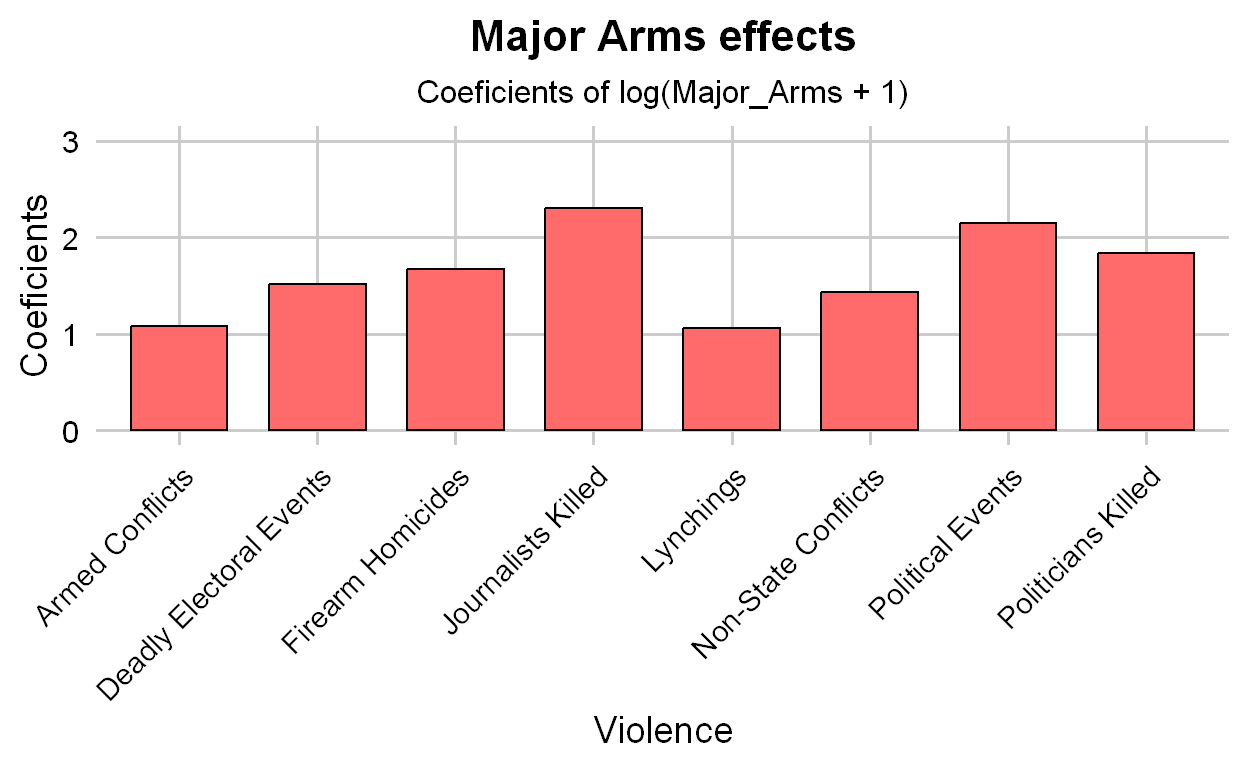
\includegraphics{Masters-Thesis--Code_files/figure-latex/unnamed-chunk-49-1.pdf}

\paragraph{4.1.2 Small arms Coeficient}\label{small-arms-coeficient}

\begin{Shaded}
\begin{Highlighting}[]
\FunctionTok{ggplot}\NormalTok{(data.graphics, }\FunctionTok{aes}\NormalTok{(}\AttributeTok{x =}\NormalTok{ Variable\_Dependiente, }\AttributeTok{y =}\NormalTok{ Small\_Arms)) }\SpecialCharTok{+}
  \FunctionTok{geom\_bar}\NormalTok{(}\AttributeTok{stat =} \StringTok{"identity"}\NormalTok{, }\AttributeTok{fill =} \StringTok{"\#BFEFFF"}\NormalTok{, }\AttributeTok{color =} \StringTok{"black"}\NormalTok{, }\AttributeTok{width =} \FloatTok{0.7}\NormalTok{) }\SpecialCharTok{+}
  \FunctionTok{theme\_minimal}\NormalTok{(}\AttributeTok{base\_size =} \DecValTok{14}\NormalTok{) }\SpecialCharTok{+}
  \FunctionTok{labs}\NormalTok{(}\AttributeTok{title =} \StringTok{"Small Arms effects"}\NormalTok{,}
       \AttributeTok{subtitle =} \StringTok{"Coeficients of log(Small\_Arms + 1)"}\NormalTok{,}
       \AttributeTok{x =} \StringTok{"Violence"}\NormalTok{,}
       \AttributeTok{y =} \StringTok{"Coeficients"}\NormalTok{) }\SpecialCharTok{+}
  \FunctionTok{ylim}\NormalTok{(}\DecValTok{0}\NormalTok{, }\DecValTok{3}\NormalTok{) }\SpecialCharTok{+}
  \FunctionTok{theme}\NormalTok{(}
    \AttributeTok{plot.title =} \FunctionTok{element\_text}\NormalTok{(}\AttributeTok{face =} \StringTok{"bold"}\NormalTok{, }\AttributeTok{hjust =} \FloatTok{0.5}\NormalTok{, }\AttributeTok{size =} \DecValTok{16}\NormalTok{),}
    \AttributeTok{plot.subtitle =} \FunctionTok{element\_text}\NormalTok{(}\AttributeTok{hjust =} \FloatTok{0.5}\NormalTok{, }\AttributeTok{size =} \DecValTok{12}\NormalTok{),}
    \AttributeTok{axis.text.x =} \FunctionTok{element\_text}\NormalTok{(}\AttributeTok{angle =} \DecValTok{45}\NormalTok{, }\AttributeTok{hjust =} \DecValTok{1}\NormalTok{),}
    \AttributeTok{axis.text =} \FunctionTok{element\_text}\NormalTok{(}\AttributeTok{color =} \StringTok{"black"}\NormalTok{),}
    \AttributeTok{panel.grid.major =} \FunctionTok{element\_line}\NormalTok{(}\AttributeTok{color =} \StringTok{"gray80"}\NormalTok{),}
    \AttributeTok{panel.grid.minor =} \FunctionTok{element\_blank}\NormalTok{()}
\NormalTok{  )}
\end{Highlighting}
\end{Shaded}

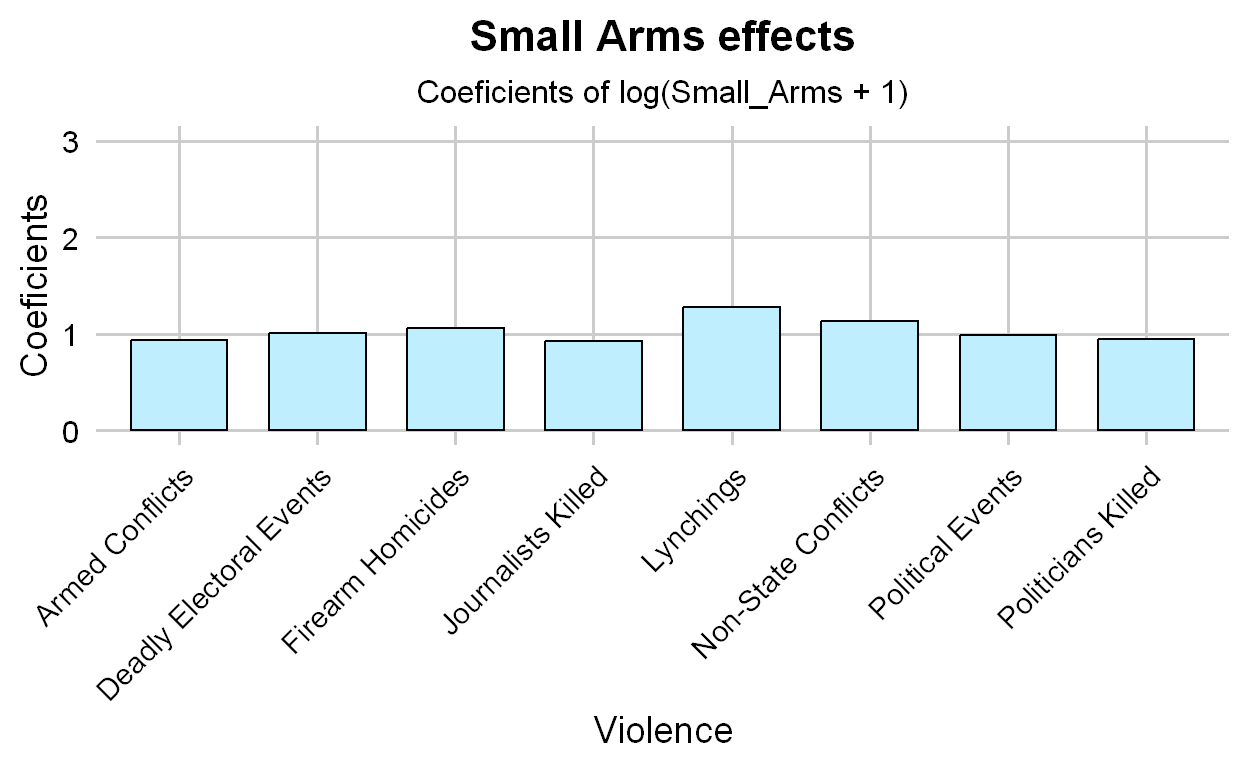
\includegraphics{Masters-Thesis--Code_files/figure-latex/unnamed-chunk-50-1.pdf}

\paragraph{4.1.3 Major and Small Arms
Coeficients}\label{major-and-small-arms-coeficients}

\begin{Shaded}
\begin{Highlighting}[]
\NormalTok{data.graphics\_long }\OtherTok{\textless{}{-}} \FunctionTok{pivot\_longer}\NormalTok{(data.graphics, }\AttributeTok{cols =} \FunctionTok{c}\NormalTok{(}\StringTok{"Major\_Arms"}\NormalTok{, }\StringTok{"Small\_Arms"}\NormalTok{), }
                          \AttributeTok{names\_to =} \StringTok{"Arms\_Type"}\NormalTok{, }\AttributeTok{values\_to =} \StringTok{"Coefficient"}\NormalTok{)}

\FunctionTok{ggplot}\NormalTok{(data.graphics\_long, }\FunctionTok{aes}\NormalTok{(}\AttributeTok{x =}\NormalTok{ Variable\_Dependiente, }\AttributeTok{y =}\NormalTok{ Coefficient, }\AttributeTok{fill =}\NormalTok{ Arms\_Type)) }\SpecialCharTok{+}
  \FunctionTok{geom\_bar}\NormalTok{(}\AttributeTok{stat =} \StringTok{"identity"}\NormalTok{, }\AttributeTok{position =} \StringTok{"dodge"}\NormalTok{, }\AttributeTok{color =} \StringTok{"black"}\NormalTok{, }\AttributeTok{width =} \FloatTok{0.7}\NormalTok{) }\SpecialCharTok{+}
  \FunctionTok{scale\_fill\_manual}\NormalTok{(}\AttributeTok{values =} \FunctionTok{c}\NormalTok{(}\StringTok{"\#FF6A6A"}\NormalTok{, }\StringTok{"\#BFEFFF"}\NormalTok{)) }\SpecialCharTok{+}  \CommentTok{\# Colores para Major Arms y Small Arms}
  \FunctionTok{theme\_minimal}\NormalTok{(}\AttributeTok{base\_size =} \DecValTok{14}\NormalTok{) }\SpecialCharTok{+}
  \FunctionTok{labs}\NormalTok{(}\AttributeTok{title =} \StringTok{"Major Arms \& Small Arms effects"}\NormalTok{,}
       \AttributeTok{subtitle =} \StringTok{"Coeficients of log(Major Arms + 1) \& log(Small Arms + 1)"}\NormalTok{,}
       \AttributeTok{x =} \StringTok{"Violence"}\NormalTok{,}
       \AttributeTok{y =} \StringTok{"Coeficients"}\NormalTok{) }\SpecialCharTok{+}
  \FunctionTok{ylim}\NormalTok{(}\DecValTok{0}\NormalTok{, }\DecValTok{3}\NormalTok{) }\SpecialCharTok{+}
  \FunctionTok{theme}\NormalTok{(}
    \AttributeTok{plot.title =} \FunctionTok{element\_text}\NormalTok{(}\AttributeTok{face =} \StringTok{"bold"}\NormalTok{, }\AttributeTok{hjust =} \FloatTok{0.5}\NormalTok{, }\AttributeTok{size =} \DecValTok{16}\NormalTok{),}
    \AttributeTok{plot.subtitle =} \FunctionTok{element\_text}\NormalTok{(}\AttributeTok{hjust =} \FloatTok{0.5}\NormalTok{, }\AttributeTok{size =} \DecValTok{12}\NormalTok{),}
    \AttributeTok{axis.text.x =} \FunctionTok{element\_text}\NormalTok{(}\AttributeTok{angle =} \DecValTok{45}\NormalTok{, }\AttributeTok{hjust =} \DecValTok{1}\NormalTok{),}
    \AttributeTok{axis.text =} \FunctionTok{element\_text}\NormalTok{(}\AttributeTok{color =} \StringTok{"black"}\NormalTok{),}
    \AttributeTok{legend.title =} \FunctionTok{element\_blank}\NormalTok{(),}
    \AttributeTok{legend.position =} \StringTok{"top"}\NormalTok{,}
    \AttributeTok{panel.grid.major =} \FunctionTok{element\_line}\NormalTok{(}\AttributeTok{color =} \StringTok{"gray80"}\NormalTok{),}
    \AttributeTok{panel.grid.minor =} \FunctionTok{element\_blank}\NormalTok{()}
\NormalTok{  )}
\end{Highlighting}
\end{Shaded}

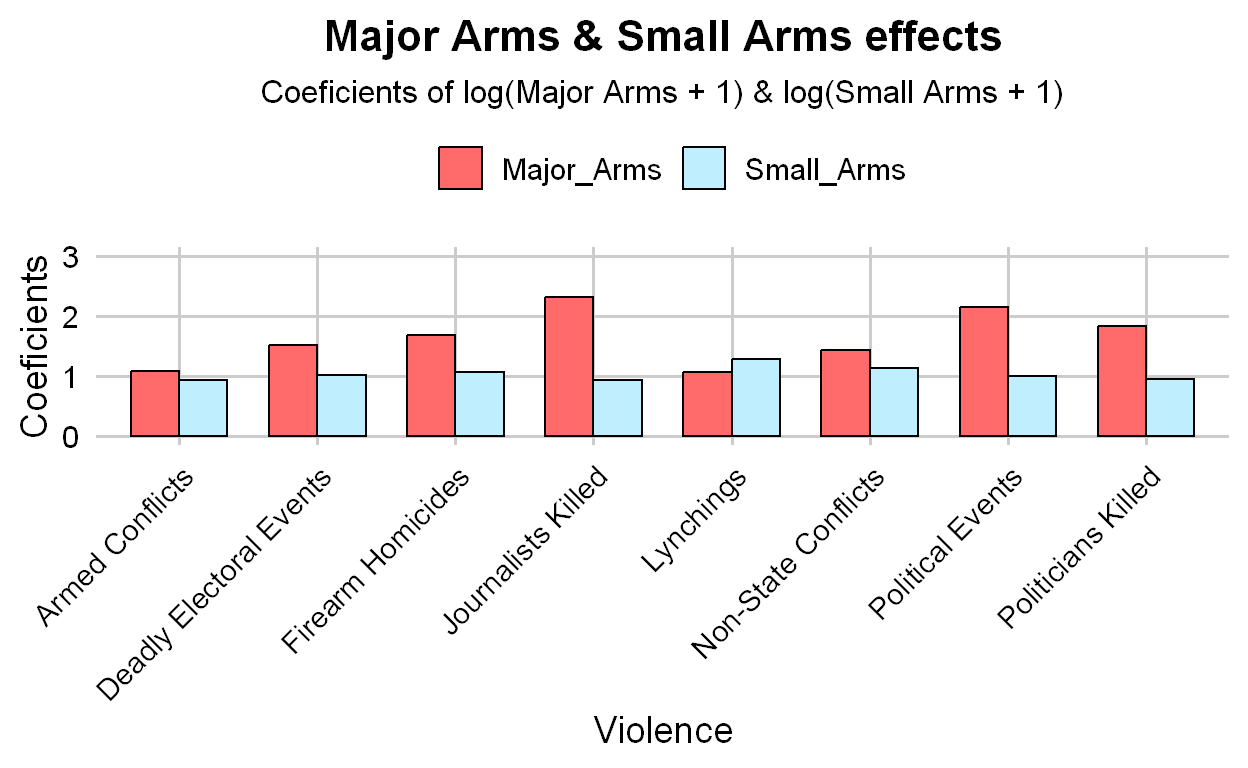
\includegraphics{Masters-Thesis--Code_files/figure-latex/unnamed-chunk-51-1.pdf}

\subsubsection{4.2 Major Arms for each
group}\label{major-arms-for-each-group}

\begin{Shaded}
\begin{Highlighting}[]
\NormalTok{General\_violence }\OtherTok{\textless{}{-}}\NormalTok{ data.graphics[data.graphics}\SpecialCharTok{$}\NormalTok{Variable\_Dependiente }\SpecialCharTok{\%in\%} \FunctionTok{c}\NormalTok{(}\StringTok{"Firearm Homicides"}\NormalTok{, }\StringTok{"Lynchings"}\NormalTok{), ]}
\NormalTok{Conflict\_Violence }\OtherTok{\textless{}{-}}\NormalTok{ data.graphics[data.graphics}\SpecialCharTok{$}\NormalTok{Variable\_Dependiente }\SpecialCharTok{\%in\%} \FunctionTok{c}\NormalTok{(}\StringTok{"Armed Conflicts"}\NormalTok{, }\StringTok{"Non{-}State Conflicts"}\NormalTok{), ]}
\NormalTok{Political\_violence }\OtherTok{\textless{}{-}}\NormalTok{ data.graphics[data.graphics}\SpecialCharTok{$}\NormalTok{Variable\_Dependiente }\SpecialCharTok{\%in\%} \FunctionTok{c}\NormalTok{(}\StringTok{"Political Events"}\NormalTok{, }\StringTok{"Deadly Electoral Events"}\NormalTok{, }\StringTok{"Journalists Killed"}\NormalTok{, }\StringTok{"Politicians Killed"}\NormalTok{), ]}
\end{Highlighting}
\end{Shaded}

\begin{Shaded}
\begin{Highlighting}[]
\FunctionTok{ggplot}\NormalTok{(General\_violence, }\FunctionTok{aes}\NormalTok{(}\AttributeTok{x =}\NormalTok{ Variable\_Dependiente, }\AttributeTok{y =}\NormalTok{ Major\_Arms)) }\SpecialCharTok{+}
  \FunctionTok{geom\_bar}\NormalTok{(}\AttributeTok{stat =} \StringTok{"identity"}\NormalTok{, }\AttributeTok{fill =} \StringTok{"\#66CDAA"}\NormalTok{, }\AttributeTok{color =} \StringTok{"black"}\NormalTok{, }\AttributeTok{width =} \FloatTok{0.6}\NormalTok{) }\SpecialCharTok{+}
  \FunctionTok{theme\_minimal}\NormalTok{(}\AttributeTok{base\_size =} \DecValTok{14}\NormalTok{) }\SpecialCharTok{+}
  \FunctionTok{labs}\NormalTok{(}\AttributeTok{title =} \StringTok{"Major Arms {-} General Violence"}\NormalTok{,}
       \AttributeTok{subtitle =} \StringTok{"Firearm Homicides \& Lynchings"}\NormalTok{,}
       \AttributeTok{x =} \StringTok{"General Violence"}\NormalTok{,}
       \AttributeTok{y =} \StringTok{"Coeficients of log(Major Arms + 1)"}\NormalTok{) }\SpecialCharTok{+}
  \FunctionTok{ylim}\NormalTok{(}\DecValTok{0}\NormalTok{, }\DecValTok{3}\NormalTok{) }\SpecialCharTok{+}
  \FunctionTok{theme}\NormalTok{(}
    \AttributeTok{plot.title =} \FunctionTok{element\_text}\NormalTok{(}\AttributeTok{face =} \StringTok{"bold"}\NormalTok{, }\AttributeTok{hjust =} \FloatTok{0.5}\NormalTok{, }\AttributeTok{size =} \DecValTok{16}\NormalTok{),}
    \AttributeTok{plot.subtitle =} \FunctionTok{element\_text}\NormalTok{(}\AttributeTok{hjust =} \FloatTok{0.5}\NormalTok{, }\AttributeTok{size =} \DecValTok{12}\NormalTok{),}
    \AttributeTok{axis.text.x =} \FunctionTok{element\_text}\NormalTok{(}\AttributeTok{angle =} \DecValTok{0}\NormalTok{, }\AttributeTok{hjust =} \FloatTok{0.5}\NormalTok{),}
    \AttributeTok{axis.text =} \FunctionTok{element\_text}\NormalTok{(}\AttributeTok{color =} \StringTok{"black"}\NormalTok{),}
    \AttributeTok{panel.grid.major =} \FunctionTok{element\_line}\NormalTok{(}\AttributeTok{color =} \StringTok{"gray80"}\NormalTok{),}
    \AttributeTok{panel.grid.minor =} \FunctionTok{element\_blank}\NormalTok{()}
\NormalTok{  )}
\end{Highlighting}
\end{Shaded}

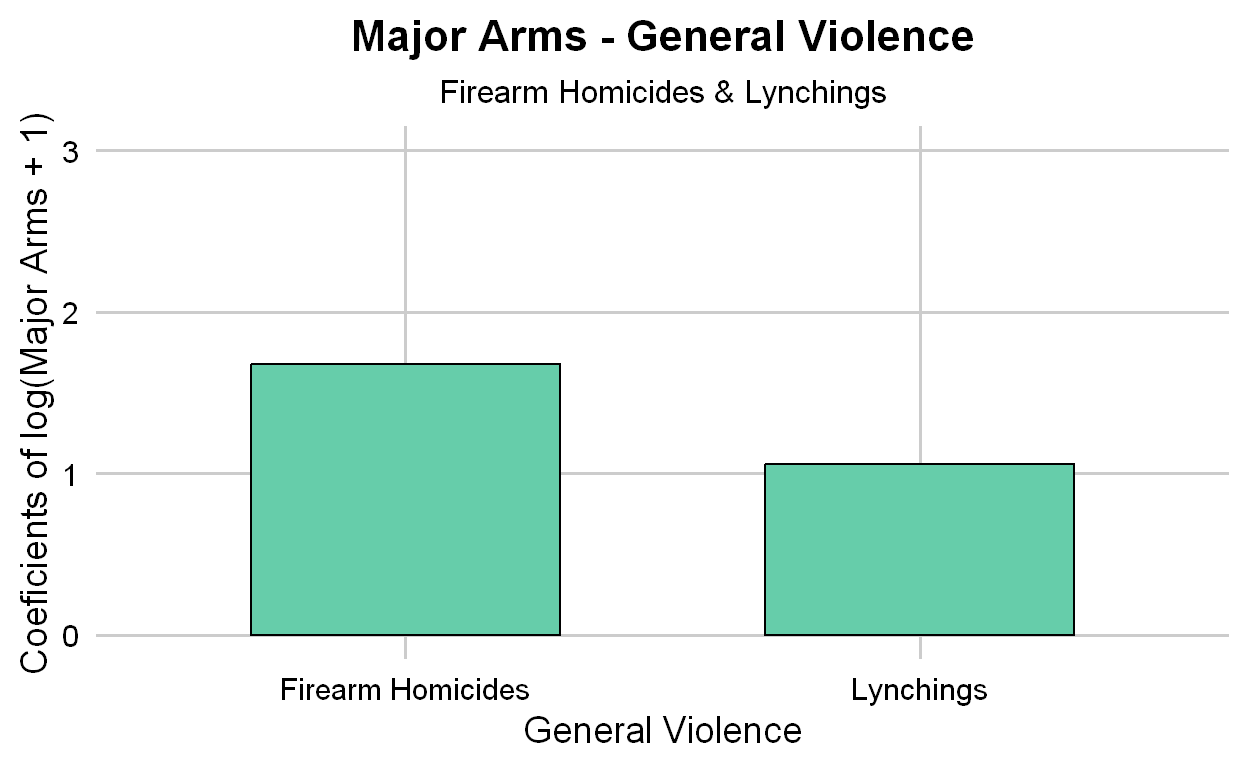
\includegraphics{Masters-Thesis--Code_files/figure-latex/unnamed-chunk-53-1.pdf}

\begin{Shaded}
\begin{Highlighting}[]
\CommentTok{\# Major Arms {-} Conflict violence}
\FunctionTok{ggplot}\NormalTok{(Conflict\_Violence, }\FunctionTok{aes}\NormalTok{(}\AttributeTok{x =}\NormalTok{ Variable\_Dependiente, }\AttributeTok{y =}\NormalTok{ Major\_Arms)) }\SpecialCharTok{+}
  \FunctionTok{geom\_bar}\NormalTok{(}\AttributeTok{stat =} \StringTok{"identity"}\NormalTok{, }\AttributeTok{fill =} \StringTok{"\#FF6A6A"}\NormalTok{, }\AttributeTok{color =} \StringTok{"black"}\NormalTok{, }\AttributeTok{width =} \FloatTok{0.6}\NormalTok{) }\SpecialCharTok{+}
  \FunctionTok{theme\_minimal}\NormalTok{(}\AttributeTok{base\_size =} \DecValTok{14}\NormalTok{) }\SpecialCharTok{+}
  \FunctionTok{labs}\NormalTok{(}\AttributeTok{title =} \StringTok{"Major Arms {-} Conflict Violence"}\NormalTok{,}
       \AttributeTok{subtitle =} \StringTok{"Armed Conflicts \& Non{-}State Conflicts"}\NormalTok{,}
       \AttributeTok{x =} \StringTok{"Conflict Violence"}\NormalTok{,}
       \AttributeTok{y =} \StringTok{"Coeficients of log(Major Arms + 1)"}\NormalTok{) }\SpecialCharTok{+}
  \FunctionTok{ylim}\NormalTok{(}\DecValTok{0}\NormalTok{, }\DecValTok{3}\NormalTok{) }\SpecialCharTok{+}
  \FunctionTok{theme}\NormalTok{(}
    \AttributeTok{plot.title =} \FunctionTok{element\_text}\NormalTok{(}\AttributeTok{face =} \StringTok{"bold"}\NormalTok{, }\AttributeTok{hjust =} \FloatTok{0.5}\NormalTok{, }\AttributeTok{size =} \DecValTok{16}\NormalTok{),}
    \AttributeTok{plot.subtitle =} \FunctionTok{element\_text}\NormalTok{(}\AttributeTok{hjust =} \FloatTok{0.5}\NormalTok{, }\AttributeTok{size =} \DecValTok{12}\NormalTok{),}
    \AttributeTok{axis.text.x =} \FunctionTok{element\_text}\NormalTok{(}\AttributeTok{angle =} \DecValTok{0}\NormalTok{, }\AttributeTok{hjust =} \FloatTok{0.5}\NormalTok{),}
    \AttributeTok{axis.text =} \FunctionTok{element\_text}\NormalTok{(}\AttributeTok{color =} \StringTok{"black"}\NormalTok{),}
    \AttributeTok{panel.grid.major =} \FunctionTok{element\_line}\NormalTok{(}\AttributeTok{color =} \StringTok{"gray80"}\NormalTok{),}
    \AttributeTok{panel.grid.minor =} \FunctionTok{element\_blank}\NormalTok{()}
\NormalTok{  )}
\end{Highlighting}
\end{Shaded}

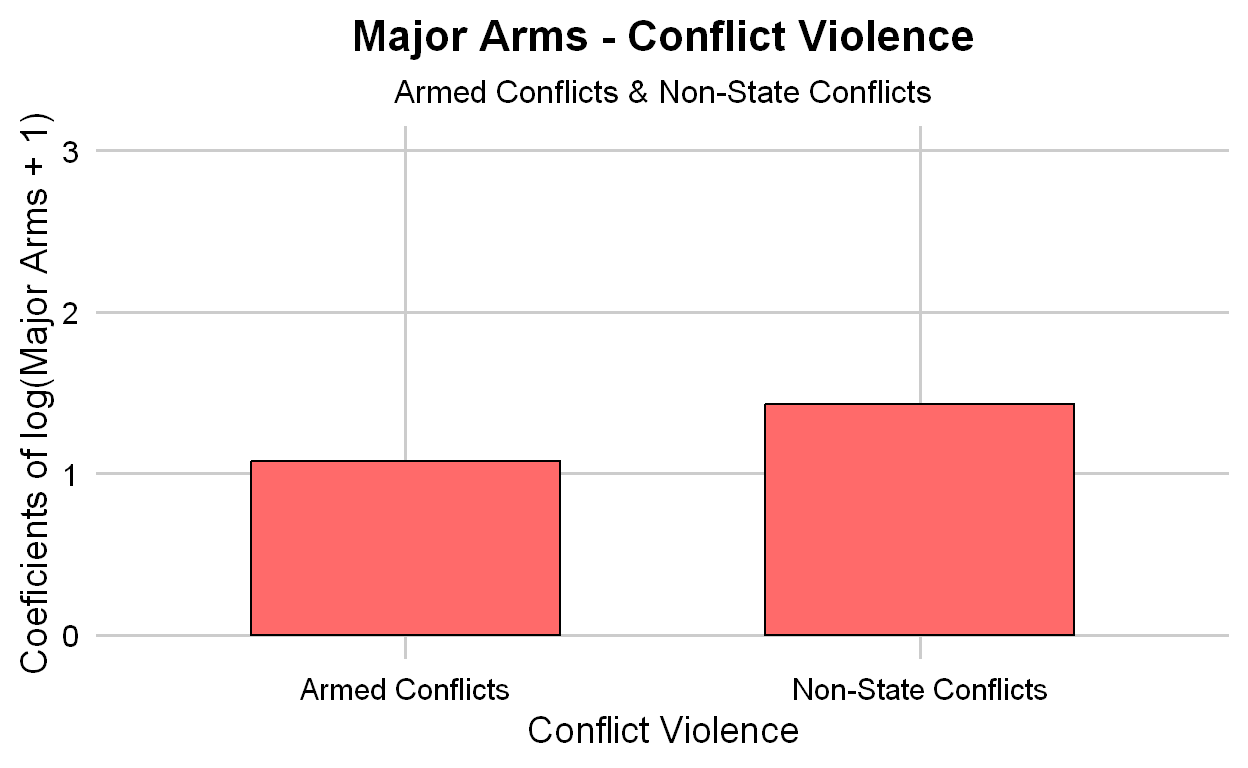
\includegraphics{Masters-Thesis--Code_files/figure-latex/unnamed-chunk-53-2.pdf}

\begin{Shaded}
\begin{Highlighting}[]
\CommentTok{\# Major Arms {-} Political violence}
\FunctionTok{ggplot}\NormalTok{(Political\_violence, }\FunctionTok{aes}\NormalTok{(}\AttributeTok{x =}\NormalTok{ Variable\_Dependiente, }\AttributeTok{y =}\NormalTok{ Major\_Arms)) }\SpecialCharTok{+}
  \FunctionTok{geom\_bar}\NormalTok{(}\AttributeTok{stat =} \StringTok{"identity"}\NormalTok{, }\AttributeTok{fill =} \StringTok{"\#BFEFFF"}\NormalTok{, }\AttributeTok{color =} \StringTok{"black"}\NormalTok{, }\AttributeTok{width =} \FloatTok{0.6}\NormalTok{) }\SpecialCharTok{+}
  \FunctionTok{theme\_minimal}\NormalTok{(}\AttributeTok{base\_size =} \DecValTok{14}\NormalTok{) }\SpecialCharTok{+}
  \FunctionTok{labs}\NormalTok{(}\AttributeTok{title =} \StringTok{"Major Arms {-} Political Violence"}\NormalTok{,}
       \AttributeTok{subtitle =} \StringTok{"Political Events, Deadly Electoral Events, Journalists Killed \& Politicians Killed"}\NormalTok{,}
       \AttributeTok{x =} \StringTok{"Political Violence"}\NormalTok{,}
       \AttributeTok{y =} \StringTok{"Coeficients of log(Major Arms + 1)"}\NormalTok{) }\SpecialCharTok{+}
  \FunctionTok{ylim}\NormalTok{(}\DecValTok{0}\NormalTok{, }\DecValTok{3}\NormalTok{) }\SpecialCharTok{+}
  \FunctionTok{theme}\NormalTok{(}
    \AttributeTok{plot.title =} \FunctionTok{element\_text}\NormalTok{(}\AttributeTok{face =} \StringTok{"bold"}\NormalTok{, }\AttributeTok{hjust =} \FloatTok{0.5}\NormalTok{, }\AttributeTok{size =} \DecValTok{16}\NormalTok{),}
    \AttributeTok{plot.subtitle =} \FunctionTok{element\_text}\NormalTok{(}\AttributeTok{hjust =} \FloatTok{0.5}\NormalTok{, }\AttributeTok{size =} \DecValTok{12}\NormalTok{),}
    \AttributeTok{axis.text.x =} \FunctionTok{element\_text}\NormalTok{(}\AttributeTok{angle =} \DecValTok{45}\NormalTok{, }\AttributeTok{hjust =} \DecValTok{1}\NormalTok{),}
    \AttributeTok{axis.text =} \FunctionTok{element\_text}\NormalTok{(}\AttributeTok{color =} \StringTok{"black"}\NormalTok{),}
    \AttributeTok{panel.grid.major =} \FunctionTok{element\_line}\NormalTok{(}\AttributeTok{color =} \StringTok{"gray80"}\NormalTok{),}
    \AttributeTok{panel.grid.minor =} \FunctionTok{element\_blank}\NormalTok{()}
\NormalTok{  )}
\end{Highlighting}
\end{Shaded}

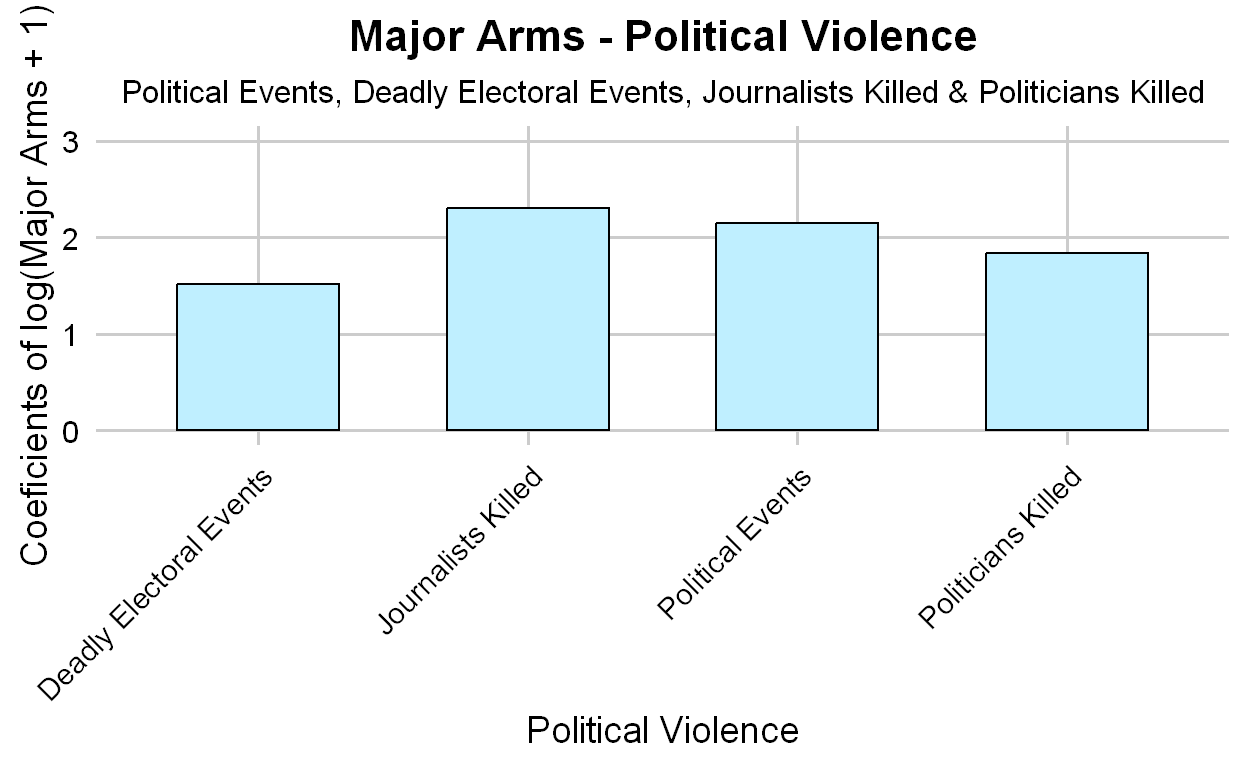
\includegraphics{Masters-Thesis--Code_files/figure-latex/unnamed-chunk-53-3.pdf}

\subsubsection{4.3 Small Arms for each
group}\label{small-arms-for-each-group}

\begin{Shaded}
\begin{Highlighting}[]
\CommentTok{\# Small Arms {-} General violence}
\FunctionTok{ggplot}\NormalTok{(General\_violence, }\FunctionTok{aes}\NormalTok{(}\AttributeTok{x =}\NormalTok{ Variable\_Dependiente, }\AttributeTok{y =}\NormalTok{ Small\_Arms)) }\SpecialCharTok{+}
  \FunctionTok{geom\_bar}\NormalTok{(}\AttributeTok{stat =} \StringTok{"identity"}\NormalTok{, }\AttributeTok{fill =} \StringTok{"\#66CDAA"}\NormalTok{, }\AttributeTok{color =} \StringTok{"black"}\NormalTok{, }\AttributeTok{width =} \FloatTok{0.6}\NormalTok{) }\SpecialCharTok{+}
  \FunctionTok{theme\_minimal}\NormalTok{(}\AttributeTok{base\_size =} \DecValTok{14}\NormalTok{) }\SpecialCharTok{+}
  \FunctionTok{labs}\NormalTok{(}\AttributeTok{title =} \StringTok{"Small Arms {-} General Violence"}\NormalTok{,}
       \AttributeTok{subtitle =} \StringTok{"Firearm Homicides \& Lynchings"}\NormalTok{,}
       \AttributeTok{x =} \StringTok{"General Violence"}\NormalTok{,}
       \AttributeTok{y =} \StringTok{"Coeficients of log(Small\_Arms + 1)"}\NormalTok{) }\SpecialCharTok{+}
  \FunctionTok{ylim}\NormalTok{(}\DecValTok{0}\NormalTok{, }\DecValTok{3}\NormalTok{) }\SpecialCharTok{+}
  \FunctionTok{theme}\NormalTok{(}
    \AttributeTok{plot.title =} \FunctionTok{element\_text}\NormalTok{(}\AttributeTok{face =} \StringTok{"bold"}\NormalTok{, }\AttributeTok{hjust =} \FloatTok{0.5}\NormalTok{, }\AttributeTok{size =} \DecValTok{16}\NormalTok{),}
    \AttributeTok{plot.subtitle =} \FunctionTok{element\_text}\NormalTok{(}\AttributeTok{hjust =} \FloatTok{0.5}\NormalTok{, }\AttributeTok{size =} \DecValTok{12}\NormalTok{),}
    \AttributeTok{axis.text.x =} \FunctionTok{element\_text}\NormalTok{(}\AttributeTok{angle =} \DecValTok{0}\NormalTok{, }\AttributeTok{hjust =} \FloatTok{0.5}\NormalTok{),}
    \AttributeTok{axis.text =} \FunctionTok{element\_text}\NormalTok{(}\AttributeTok{color =} \StringTok{"black"}\NormalTok{),}
    \AttributeTok{panel.grid.major =} \FunctionTok{element\_line}\NormalTok{(}\AttributeTok{color =} \StringTok{"gray80"}\NormalTok{),}
    \AttributeTok{panel.grid.minor =} \FunctionTok{element\_blank}\NormalTok{()}
\NormalTok{  )}
\end{Highlighting}
\end{Shaded}

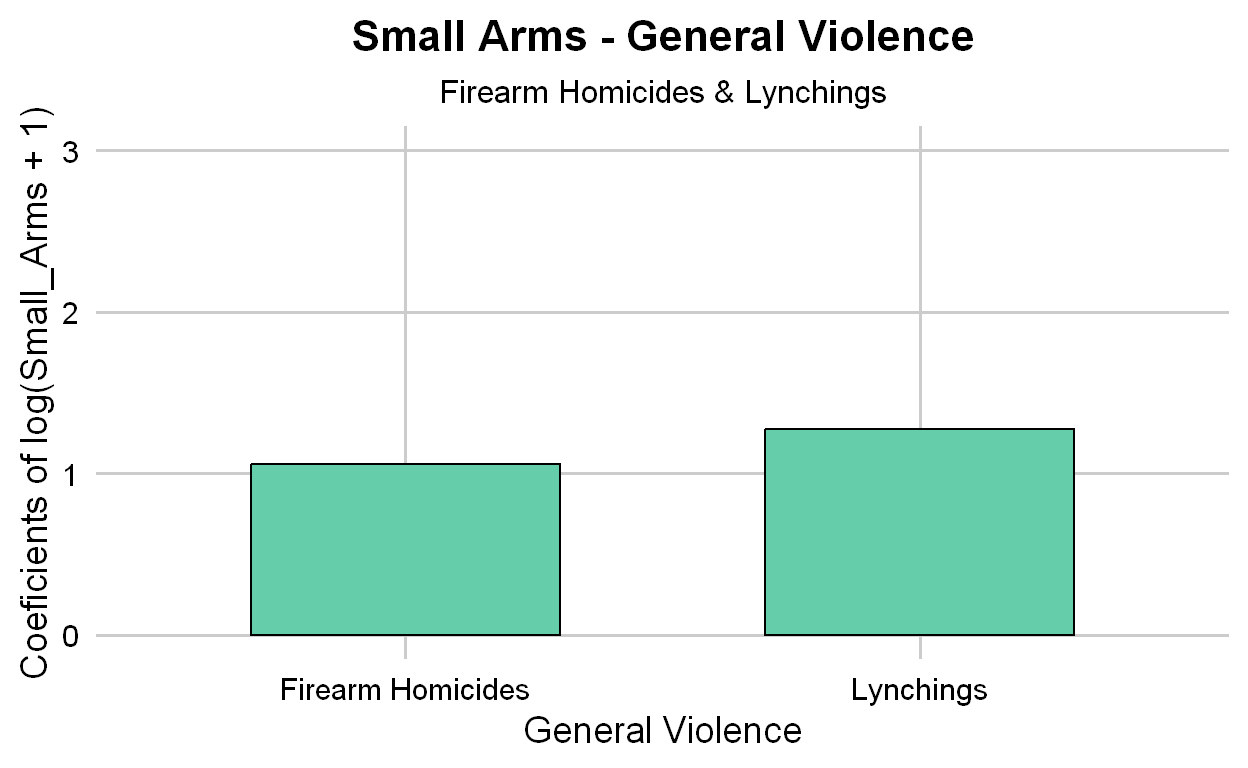
\includegraphics{Masters-Thesis--Code_files/figure-latex/unnamed-chunk-54-1.pdf}

\begin{Shaded}
\begin{Highlighting}[]
\CommentTok{\# Small Arms {-} Conflict violence}
\FunctionTok{ggplot}\NormalTok{(Conflict\_Violence, }\FunctionTok{aes}\NormalTok{(}\AttributeTok{x =}\NormalTok{ Variable\_Dependiente, }\AttributeTok{y =}\NormalTok{ Small\_Arms)) }\SpecialCharTok{+}
  \FunctionTok{geom\_bar}\NormalTok{(}\AttributeTok{stat =} \StringTok{"identity"}\NormalTok{, }\AttributeTok{fill =} \StringTok{"\#FF6A6A"}\NormalTok{, }\AttributeTok{color =} \StringTok{"black"}\NormalTok{, }\AttributeTok{width =} \FloatTok{0.6}\NormalTok{) }\SpecialCharTok{+}
  \FunctionTok{theme\_minimal}\NormalTok{(}\AttributeTok{base\_size =} \DecValTok{14}\NormalTok{) }\SpecialCharTok{+}
  \FunctionTok{labs}\NormalTok{(}\AttributeTok{title =} \StringTok{"Small Arms {-} Conflict Violence"}\NormalTok{,}
       \AttributeTok{subtitle =} \StringTok{"Armed Conflicts \& Non{-}State Conflicts"}\NormalTok{,}
       \AttributeTok{x =} \StringTok{"Conflict Violence"}\NormalTok{,}
       \AttributeTok{y =} \StringTok{"Coeficients of log(Small\_Arms + 1)"}\NormalTok{) }\SpecialCharTok{+}
  \FunctionTok{ylim}\NormalTok{(}\DecValTok{0}\NormalTok{, }\DecValTok{3}\NormalTok{) }\SpecialCharTok{+}
  \FunctionTok{theme}\NormalTok{(}
    \AttributeTok{plot.title =} \FunctionTok{element\_text}\NormalTok{(}\AttributeTok{face =} \StringTok{"bold"}\NormalTok{, }\AttributeTok{hjust =} \FloatTok{0.5}\NormalTok{, }\AttributeTok{size =} \DecValTok{16}\NormalTok{),}
    \AttributeTok{plot.subtitle =} \FunctionTok{element\_text}\NormalTok{(}\AttributeTok{hjust =} \FloatTok{0.5}\NormalTok{, }\AttributeTok{size =} \DecValTok{12}\NormalTok{),}
    \AttributeTok{axis.text.x =} \FunctionTok{element\_text}\NormalTok{(}\AttributeTok{angle =} \DecValTok{0}\NormalTok{, }\AttributeTok{hjust =} \FloatTok{0.5}\NormalTok{),}
    \AttributeTok{axis.text =} \FunctionTok{element\_text}\NormalTok{(}\AttributeTok{color =} \StringTok{"black"}\NormalTok{),}
    \AttributeTok{panel.grid.major =} \FunctionTok{element\_line}\NormalTok{(}\AttributeTok{color =} \StringTok{"gray80"}\NormalTok{),}
    \AttributeTok{panel.grid.minor =} \FunctionTok{element\_blank}\NormalTok{()}
\NormalTok{  )}
\end{Highlighting}
\end{Shaded}

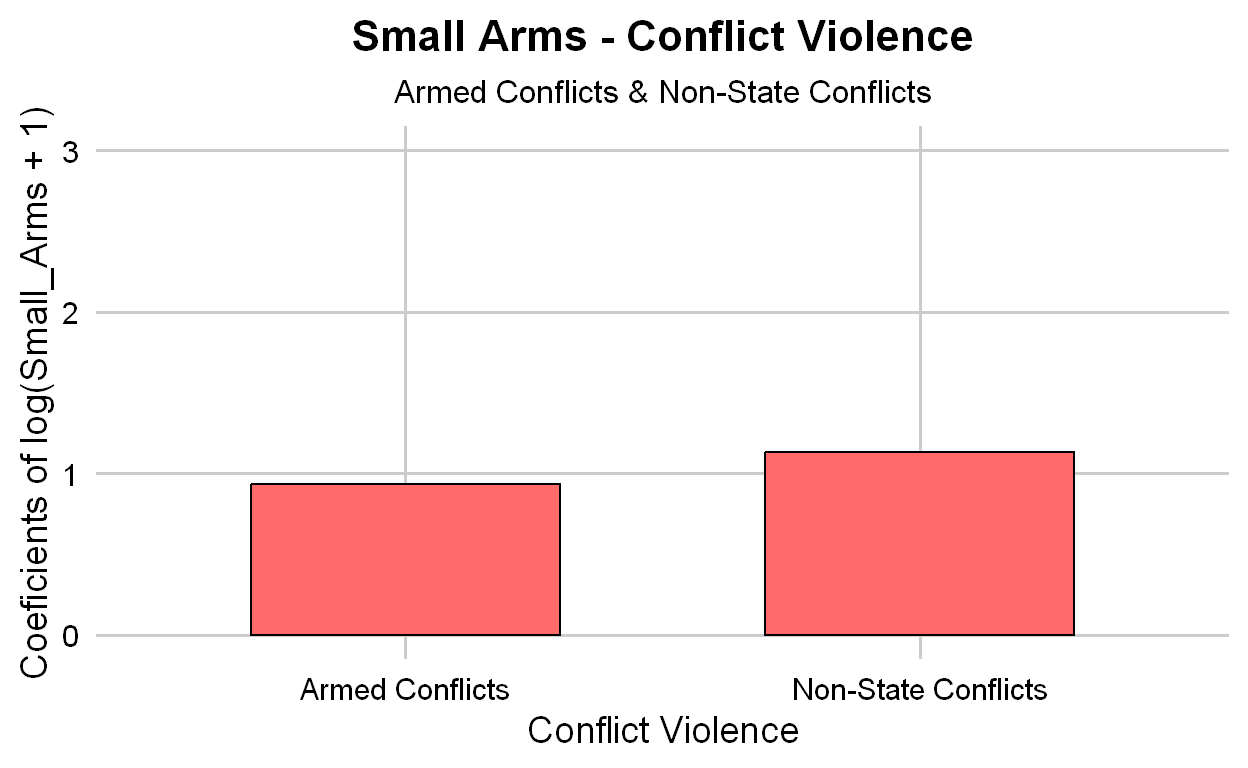
\includegraphics{Masters-Thesis--Code_files/figure-latex/unnamed-chunk-54-2.pdf}

\begin{Shaded}
\begin{Highlighting}[]
\CommentTok{\# Small Arms {-} Political violence}
\FunctionTok{ggplot}\NormalTok{(Political\_violence, }\FunctionTok{aes}\NormalTok{(}\AttributeTok{x =}\NormalTok{ Variable\_Dependiente, }\AttributeTok{y =}\NormalTok{ Small\_Arms)) }\SpecialCharTok{+}
  \FunctionTok{geom\_bar}\NormalTok{(}\AttributeTok{stat =} \StringTok{"identity"}\NormalTok{, }\AttributeTok{fill =} \StringTok{"\#BFEFFF"}\NormalTok{, }\AttributeTok{color =} \StringTok{"black"}\NormalTok{, }\AttributeTok{width =} \FloatTok{0.6}\NormalTok{) }\SpecialCharTok{+}
  \FunctionTok{theme\_minimal}\NormalTok{(}\AttributeTok{base\_size =} \DecValTok{14}\NormalTok{) }\SpecialCharTok{+}
  \FunctionTok{labs}\NormalTok{(}\AttributeTok{title =} \StringTok{"Small Arms {-} Political Violence"}\NormalTok{,}
       \AttributeTok{subtitle =} \StringTok{"Political Events, Deadly Electoral Events, Journalists Killed \& Politicians Killed"}\NormalTok{,}
       \AttributeTok{x =} \StringTok{"Political Violence"}\NormalTok{,}
       \AttributeTok{y =} \StringTok{"Coeficients of log(Small\_Arms + 1)"}\NormalTok{) }\SpecialCharTok{+}
  \FunctionTok{ylim}\NormalTok{(}\DecValTok{0}\NormalTok{, }\DecValTok{3}\NormalTok{) }\SpecialCharTok{+}
  \FunctionTok{theme}\NormalTok{(}
    \AttributeTok{plot.title =} \FunctionTok{element\_text}\NormalTok{(}\AttributeTok{face =} \StringTok{"bold"}\NormalTok{, }\AttributeTok{hjust =} \FloatTok{0.5}\NormalTok{, }\AttributeTok{size =} \DecValTok{16}\NormalTok{),}
    \AttributeTok{plot.subtitle =} \FunctionTok{element\_text}\NormalTok{(}\AttributeTok{hjust =} \FloatTok{0.5}\NormalTok{, }\AttributeTok{size =} \DecValTok{12}\NormalTok{),}
    \AttributeTok{axis.text.x =} \FunctionTok{element\_text}\NormalTok{(}\AttributeTok{angle =} \DecValTok{45}\NormalTok{, }\AttributeTok{hjust =} \DecValTok{1}\NormalTok{),}
    \AttributeTok{axis.text =} \FunctionTok{element\_text}\NormalTok{(}\AttributeTok{color =} \StringTok{"black"}\NormalTok{),}
    \AttributeTok{panel.grid.major =} \FunctionTok{element\_line}\NormalTok{(}\AttributeTok{color =} \StringTok{"gray80"}\NormalTok{),}
    \AttributeTok{panel.grid.minor =} \FunctionTok{element\_blank}\NormalTok{()}
\NormalTok{  )}
\end{Highlighting}
\end{Shaded}

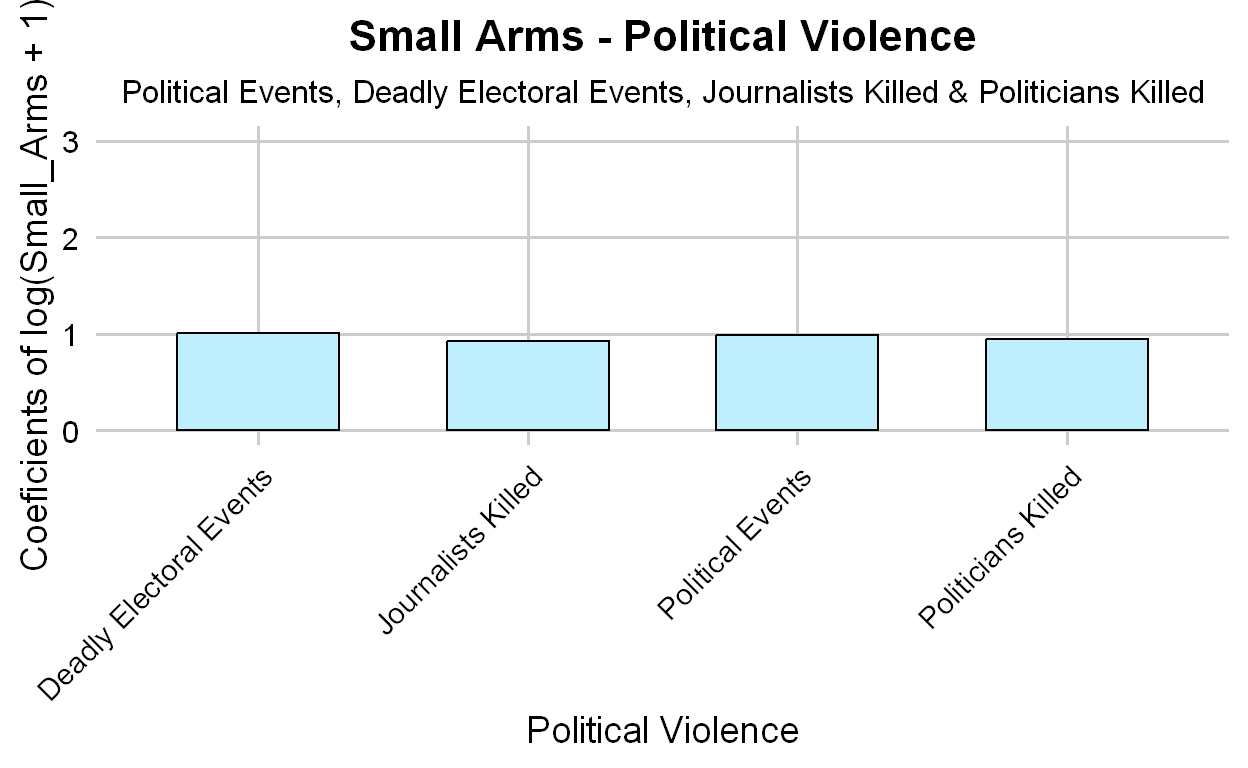
\includegraphics{Masters-Thesis--Code_files/figure-latex/unnamed-chunk-54-3.pdf}

\subsubsection{4.4 Major Arms by groups}\label{major-arms-by-groups}

\begin{Shaded}
\begin{Highlighting}[]
\NormalTok{data.graphics.grouped }\OtherTok{\textless{}{-}} \FunctionTok{data.frame}\NormalTok{(}
  \AttributeTok{Variable\_Dependiente =} \FunctionTok{c}\NormalTok{(}\StringTok{"Firearm Homicides"}\NormalTok{, }\StringTok{"Lynchings"}\NormalTok{, }\StringTok{"Armed Conflicts"}\NormalTok{, }
                           \StringTok{"Non{-}State Conflicts"}\NormalTok{, }\StringTok{"Political Events"}\NormalTok{, }\StringTok{"Deadly Electoral Events"}\NormalTok{, }
                           \StringTok{"Journalists Killed"}\NormalTok{, }\StringTok{"Politicians Killed"}\NormalTok{),}
  \AttributeTok{Major\_Arms =} \FunctionTok{c}\NormalTok{(}\FloatTok{1.674322}\NormalTok{, }\FloatTok{1.059879}\NormalTok{, }\FloatTok{1.0758477}\NormalTok{, }\FloatTok{1.4303096}\NormalTok{, }\FloatTok{2.1480569}\NormalTok{, }\FloatTok{1.51709125}\NormalTok{, }\FloatTok{2.30727437}\NormalTok{, }\FloatTok{1.8319250}\NormalTok{),}
  \AttributeTok{Small\_Arms =} \FunctionTok{c}\NormalTok{(}\FloatTok{1.057475}\NormalTok{, }\FloatTok{1.273150}\NormalTok{, }\FloatTok{0.9359766}\NormalTok{, }\FloatTok{1.1322211}\NormalTok{, }\FloatTok{0.9898447}\NormalTok{, }\FloatTok{1.00487220}\NormalTok{, }\FloatTok{0.92587390}\NormalTok{, }\FloatTok{0.9440187}\NormalTok{),}
  \AttributeTok{Group =} \FunctionTok{c}\NormalTok{(}\StringTok{"General violence"}\NormalTok{, }\StringTok{"General violence"}\NormalTok{, }
            \StringTok{"Conflict Violence"}\NormalTok{, }\StringTok{"Conflict Violence"}\NormalTok{, }
            \StringTok{"Political violence"}\NormalTok{, }\StringTok{"Political violence"}\NormalTok{, }
            \StringTok{"Political violence"}\NormalTok{, }\StringTok{"Political violence"}\NormalTok{)}
\NormalTok{)}

\NormalTok{data.graphics.grouped}\SpecialCharTok{$}\NormalTok{Group }\OtherTok{\textless{}{-}} \FunctionTok{factor}\NormalTok{(data.graphics.grouped}\SpecialCharTok{$}\NormalTok{Group, }
                                      \AttributeTok{levels =} \FunctionTok{c}\NormalTok{(}\StringTok{"General violence"}\NormalTok{, }\StringTok{"Conflict Violence"}\NormalTok{, }\StringTok{"Political violence"}\NormalTok{))}

\NormalTok{data.graphics.grouped}\SpecialCharTok{$}\NormalTok{Variable\_Dependiente }\OtherTok{\textless{}{-}} \FunctionTok{factor}\NormalTok{(data.graphics.grouped}\SpecialCharTok{$}\NormalTok{Variable\_Dependiente, }
                                                     \AttributeTok{levels =}\NormalTok{ data.graphics.grouped}\SpecialCharTok{$}\NormalTok{Variable\_Dependiente[}\FunctionTok{order}\NormalTok{(data.graphics.grouped}\SpecialCharTok{$}\NormalTok{Group)])}

\FunctionTok{ggplot}\NormalTok{(data.graphics.grouped, }\FunctionTok{aes}\NormalTok{(}\AttributeTok{x =}\NormalTok{ Variable\_Dependiente, }\AttributeTok{y =}\NormalTok{ Major\_Arms, }\AttributeTok{fill =}\NormalTok{ Group)) }\SpecialCharTok{+}
  \FunctionTok{geom\_bar}\NormalTok{(}\AttributeTok{stat =} \StringTok{"identity"}\NormalTok{, }\AttributeTok{color =} \StringTok{"black"}\NormalTok{, }\AttributeTok{width =} \FloatTok{0.7}\NormalTok{, }\AttributeTok{position =} \FunctionTok{position\_dodge}\NormalTok{()) }\SpecialCharTok{+}
  \FunctionTok{scale\_fill\_manual}\NormalTok{(}\AttributeTok{values =} \FunctionTok{c}\NormalTok{(}\StringTok{"General violence"} \OtherTok{=} \StringTok{"\#66CDAA"}\NormalTok{, }\StringTok{"Conflict Violence"} \OtherTok{=} \StringTok{"\#FF6A6A"}\NormalTok{, }\StringTok{"Political violence"} \OtherTok{=} \StringTok{"\#BFEFFF"}\NormalTok{)) }\SpecialCharTok{+}
  \FunctionTok{theme\_minimal}\NormalTok{(}\AttributeTok{base\_size =} \DecValTok{14}\NormalTok{) }\SpecialCharTok{+}
  \FunctionTok{labs}\NormalTok{(}\AttributeTok{title =} \StringTok{"Major Arms by Groups"}\NormalTok{,}
       \AttributeTok{subtitle =} \StringTok{"Coeficients of log(Major\_Arms + 1)"}\NormalTok{,}
       \AttributeTok{x =} \StringTok{"Violence"}\NormalTok{,}
       \AttributeTok{y =} \StringTok{"Coeficients"}\NormalTok{) }\SpecialCharTok{+}
  \FunctionTok{ylim}\NormalTok{(}\DecValTok{0}\NormalTok{, }\DecValTok{3}\NormalTok{) }\SpecialCharTok{+}
  \FunctionTok{theme}\NormalTok{(}
    \AttributeTok{plot.title =} \FunctionTok{element\_text}\NormalTok{(}\AttributeTok{face =} \StringTok{"bold"}\NormalTok{, }\AttributeTok{hjust =} \FloatTok{0.5}\NormalTok{, }\AttributeTok{size =} \DecValTok{16}\NormalTok{),}
    \AttributeTok{plot.subtitle =} \FunctionTok{element\_text}\NormalTok{(}\AttributeTok{hjust =} \FloatTok{0.5}\NormalTok{, }\AttributeTok{size =} \DecValTok{12}\NormalTok{),}
    \AttributeTok{axis.text.x =} \FunctionTok{element\_text}\NormalTok{(}\AttributeTok{angle =} \DecValTok{45}\NormalTok{, }\AttributeTok{hjust =} \DecValTok{1}\NormalTok{),}
    \AttributeTok{axis.text =} \FunctionTok{element\_text}\NormalTok{(}\AttributeTok{color =} \StringTok{"black"}\NormalTok{),}
    \AttributeTok{panel.grid.major =} \FunctionTok{element\_line}\NormalTok{(}\AttributeTok{color =} \StringTok{"gray80"}\NormalTok{),}
    \AttributeTok{panel.grid.minor =} \FunctionTok{element\_blank}\NormalTok{(),}
    \AttributeTok{legend.position =} \StringTok{"top"}
\NormalTok{  )}
\end{Highlighting}
\end{Shaded}

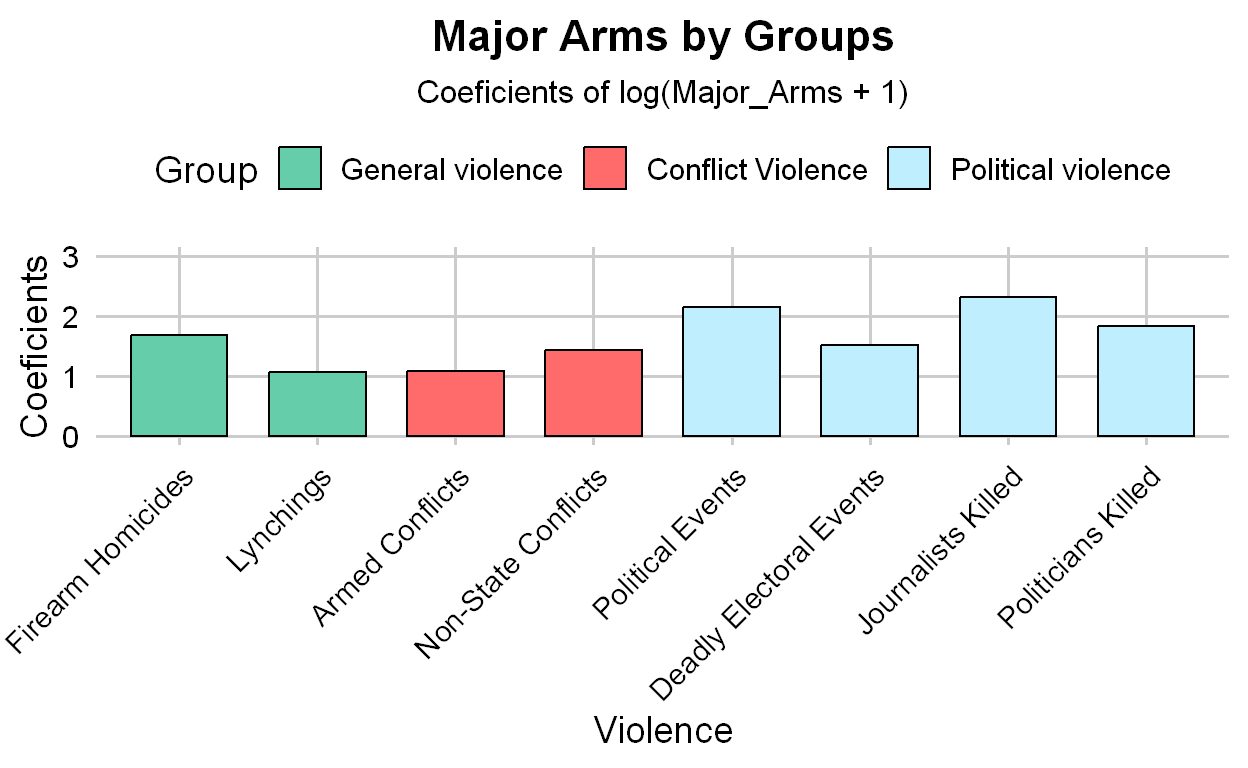
\includegraphics{Masters-Thesis--Code_files/figure-latex/unnamed-chunk-55-1.pdf}

\subsubsection{4.5 Small Arms by groups}\label{small-arms-by-groups}

\begin{Shaded}
\begin{Highlighting}[]
\NormalTok{data.graphics.grouped }\OtherTok{\textless{}{-}} \FunctionTok{data.frame}\NormalTok{(}
  \AttributeTok{Variable\_Dependiente =} \FunctionTok{c}\NormalTok{(}\StringTok{"Firearm Homicides"}\NormalTok{, }\StringTok{"Lynchings"}\NormalTok{, }\StringTok{"Armed Conflicts"}\NormalTok{, }
                           \StringTok{"Non{-}State Conflicts"}\NormalTok{, }\StringTok{"Political Events"}\NormalTok{, }\StringTok{"Deadly Electoral Events"}\NormalTok{, }
                           \StringTok{"Journalists Killed"}\NormalTok{, }\StringTok{"Politicians Killed"}\NormalTok{),}
  \AttributeTok{Major\_Arms =} \FunctionTok{c}\NormalTok{(}\FloatTok{1.674322}\NormalTok{, }\FloatTok{1.059879}\NormalTok{, }\FloatTok{1.0758477}\NormalTok{, }\FloatTok{1.4303096}\NormalTok{, }\FloatTok{2.1480569}\NormalTok{, }\FloatTok{1.51709125}\NormalTok{, }\FloatTok{2.30727437}\NormalTok{, }\FloatTok{1.8319250}\NormalTok{),}
  \AttributeTok{Small\_Arms =} \FunctionTok{c}\NormalTok{(}\FloatTok{1.057475}\NormalTok{, }\FloatTok{1.273150}\NormalTok{, }\FloatTok{0.9359766}\NormalTok{, }\FloatTok{1.1322211}\NormalTok{, }\FloatTok{0.9898447}\NormalTok{, }\FloatTok{1.00487220}\NormalTok{, }\FloatTok{0.92587390}\NormalTok{, }\FloatTok{0.9440187}\NormalTok{),}
  \AttributeTok{Group =} \FunctionTok{c}\NormalTok{(}\StringTok{"General violence"}\NormalTok{, }\StringTok{"General violence"}\NormalTok{, }
            \StringTok{"Conflict Violence"}\NormalTok{, }\StringTok{"Conflict Violence"}\NormalTok{, }
            \StringTok{"Political violence"}\NormalTok{, }\StringTok{"Political violence"}\NormalTok{, }
            \StringTok{"Political violence"}\NormalTok{, }\StringTok{"Political violence"}\NormalTok{)}
\NormalTok{)}

\NormalTok{data.graphics.grouped}\SpecialCharTok{$}\NormalTok{Group }\OtherTok{\textless{}{-}} \FunctionTok{factor}\NormalTok{(data.graphics.grouped}\SpecialCharTok{$}\NormalTok{Group, }
                                      \AttributeTok{levels =} \FunctionTok{c}\NormalTok{(}\StringTok{"General violence"}\NormalTok{, }\StringTok{"Conflict Violence"}\NormalTok{, }\StringTok{"Political violence"}\NormalTok{))}

\NormalTok{data.graphics.grouped}\SpecialCharTok{$}\NormalTok{Variable\_Dependiente }\OtherTok{\textless{}{-}} \FunctionTok{factor}\NormalTok{(data.graphics.grouped}\SpecialCharTok{$}\NormalTok{Variable\_Dependiente, }
                                                     \AttributeTok{levels =}\NormalTok{ data.graphics.grouped}\SpecialCharTok{$}\NormalTok{Variable\_Dependiente[}\FunctionTok{order}\NormalTok{(data.graphics.grouped}\SpecialCharTok{$}\NormalTok{Group)])}

\FunctionTok{ggplot}\NormalTok{(data.graphics.grouped, }\FunctionTok{aes}\NormalTok{(}\AttributeTok{x =}\NormalTok{ Variable\_Dependiente, }\AttributeTok{y =}\NormalTok{ Small\_Arms, }\AttributeTok{fill =}\NormalTok{ Group)) }\SpecialCharTok{+}
  \FunctionTok{geom\_bar}\NormalTok{(}\AttributeTok{stat =} \StringTok{"identity"}\NormalTok{, }\AttributeTok{color =} \StringTok{"black"}\NormalTok{, }\AttributeTok{width =} \FloatTok{0.7}\NormalTok{, }\AttributeTok{position =} \FunctionTok{position\_dodge}\NormalTok{()) }\SpecialCharTok{+}
  \FunctionTok{scale\_fill\_manual}\NormalTok{(}\AttributeTok{values =} \FunctionTok{c}\NormalTok{(}\StringTok{"General violence"} \OtherTok{=} \StringTok{"\#66CDAA"}\NormalTok{, }\StringTok{"Conflict Violence"} \OtherTok{=} \StringTok{"\#FF6A6A"}\NormalTok{, }\StringTok{"Political violence"} \OtherTok{=} \StringTok{"\#BFEFFF"}\NormalTok{)) }\SpecialCharTok{+}
  \FunctionTok{theme\_minimal}\NormalTok{(}\AttributeTok{base\_size =} \DecValTok{14}\NormalTok{) }\SpecialCharTok{+}
  \FunctionTok{labs}\NormalTok{(}\AttributeTok{title =} \StringTok{"Small Arms by Groups"}\NormalTok{,}
       \AttributeTok{subtitle =} \StringTok{"Coeficients of log(Small\_Arms + 1)"}\NormalTok{,}
       \AttributeTok{x =} \StringTok{"Violence"}\NormalTok{,}
       \AttributeTok{y =} \StringTok{"Coeficients"}\NormalTok{) }\SpecialCharTok{+}
  \FunctionTok{ylim}\NormalTok{(}\DecValTok{0}\NormalTok{, }\DecValTok{3}\NormalTok{) }\SpecialCharTok{+}
  \FunctionTok{theme}\NormalTok{(}
    \AttributeTok{plot.title =} \FunctionTok{element\_text}\NormalTok{(}\AttributeTok{face =} \StringTok{"bold"}\NormalTok{, }\AttributeTok{hjust =} \FloatTok{0.5}\NormalTok{, }\AttributeTok{size =} \DecValTok{16}\NormalTok{),}
    \AttributeTok{plot.subtitle =} \FunctionTok{element\_text}\NormalTok{(}\AttributeTok{hjust =} \FloatTok{0.5}\NormalTok{, }\AttributeTok{size =} \DecValTok{12}\NormalTok{),}
    \AttributeTok{axis.text.x =} \FunctionTok{element\_text}\NormalTok{(}\AttributeTok{angle =} \DecValTok{45}\NormalTok{, }\AttributeTok{hjust =} \DecValTok{1}\NormalTok{),}
    \AttributeTok{axis.text =} \FunctionTok{element\_text}\NormalTok{(}\AttributeTok{color =} \StringTok{"black"}\NormalTok{),}
    \AttributeTok{panel.grid.major =} \FunctionTok{element\_line}\NormalTok{(}\AttributeTok{color =} \StringTok{"gray80"}\NormalTok{),}
    \AttributeTok{panel.grid.minor =} \FunctionTok{element\_blank}\NormalTok{(),}
    \AttributeTok{legend.position =} \StringTok{"top"}
\NormalTok{  )}
\end{Highlighting}
\end{Shaded}

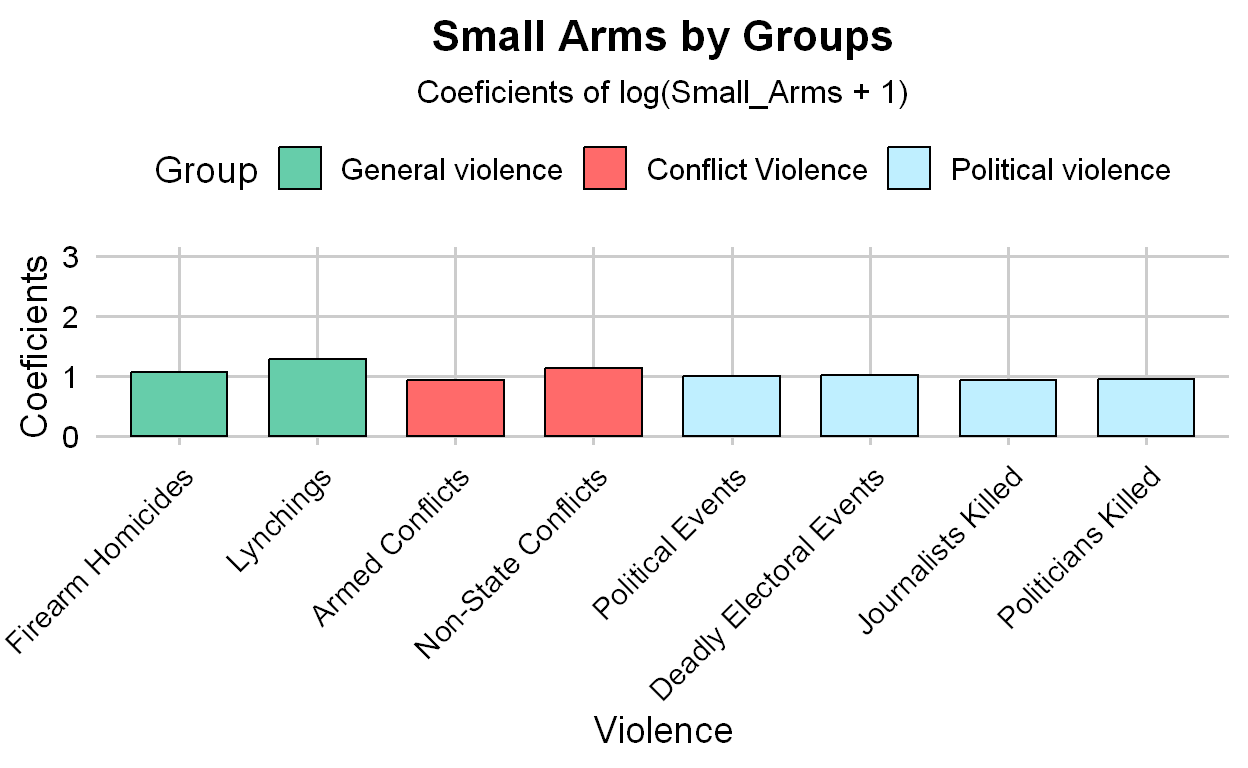
\includegraphics{Masters-Thesis--Code_files/figure-latex/unnamed-chunk-56-1.pdf}

\end{document}
